\documentclass[twoside]{book}

% Packages required by doxygen
\usepackage{fixltx2e}
\usepackage{calc}
\usepackage{doxygen}
\usepackage[export]{adjustbox} % also loads graphicx
\usepackage{graphicx}
\usepackage[utf8]{inputenc}
\usepackage{makeidx}
\usepackage{multicol}
\usepackage{multirow}
\PassOptionsToPackage{warn}{textcomp}
\usepackage{textcomp}
\usepackage[nointegrals]{wasysym}
\usepackage[table]{xcolor}

% Font selection
\usepackage[T1]{fontenc}
\usepackage[scaled=.90]{helvet}
\usepackage{courier}
\usepackage{amssymb}
\usepackage{sectsty}
\renewcommand{\familydefault}{\sfdefault}
\allsectionsfont{%
  \fontseries{bc}\selectfont%
  \color{darkgray}%
}
\renewcommand{\DoxyLabelFont}{%
  \fontseries{bc}\selectfont%
  \color{darkgray}%
}
\newcommand{\+}{\discretionary{\mbox{\scriptsize$\hookleftarrow$}}{}{}}

% Page & text layout
\usepackage{geometry}
\geometry{%
  a4paper,%
  top=2.5cm,%
  bottom=2.5cm,%
  left=2.5cm,%
  right=2.5cm%
}
\tolerance=750
\hfuzz=15pt
\hbadness=750
\setlength{\emergencystretch}{15pt}
\setlength{\parindent}{0cm}
\setlength{\parskip}{3ex plus 2ex minus 2ex}
\makeatletter
\renewcommand{\paragraph}{%
  \@startsection{paragraph}{4}{0ex}{-1.0ex}{1.0ex}{%
    \normalfont\normalsize\bfseries\SS@parafont%
  }%
}
\renewcommand{\subparagraph}{%
  \@startsection{subparagraph}{5}{0ex}{-1.0ex}{1.0ex}{%
    \normalfont\normalsize\bfseries\SS@subparafont%
  }%
}
\makeatother

% Headers & footers
\usepackage{fancyhdr}
\pagestyle{fancyplain}
\fancyhead[LE]{\fancyplain{}{\bfseries\thepage}}
\fancyhead[CE]{\fancyplain{}{}}
\fancyhead[RE]{\fancyplain{}{\bfseries\leftmark}}
\fancyhead[LO]{\fancyplain{}{\bfseries\rightmark}}
\fancyhead[CO]{\fancyplain{}{}}
\fancyhead[RO]{\fancyplain{}{\bfseries\thepage}}
\fancyfoot[LE]{\fancyplain{}{}}
\fancyfoot[CE]{\fancyplain{}{}}
\fancyfoot[RE]{\fancyplain{}{\bfseries\scriptsize Generated by Doxygen }}
\fancyfoot[LO]{\fancyplain{}{\bfseries\scriptsize Generated by Doxygen }}
\fancyfoot[CO]{\fancyplain{}{}}
\fancyfoot[RO]{\fancyplain{}{}}
\renewcommand{\footrulewidth}{0.4pt}
\renewcommand{\chaptermark}[1]{%
  \markboth{#1}{}%
}
\renewcommand{\sectionmark}[1]{%
  \markright{\thesection\ #1}%
}

% Indices & bibliography
\usepackage{natbib}
\usepackage[titles]{tocloft}
\setcounter{tocdepth}{3}
\setcounter{secnumdepth}{5}
\makeindex

% Hyperlinks (required, but should be loaded last)
\usepackage{ifpdf}
\ifpdf
  \usepackage[pdftex,pagebackref=true]{hyperref}
\else
  \usepackage[ps2pdf,pagebackref=true]{hyperref}
\fi
\hypersetup{%
  colorlinks=true,%
  linkcolor=blue,%
  citecolor=blue,%
  unicode%
}

% Custom commands
\newcommand{\clearemptydoublepage}{%
  \newpage{\pagestyle{empty}\cleardoublepage}%
}

\usepackage{caption}
\captionsetup{labelsep=space,justification=centering,font={bf},singlelinecheck=off,skip=4pt,position=top}

%===== C O N T E N T S =====

\begin{document}

% Titlepage & ToC
\hypersetup{pageanchor=false,
             bookmarksnumbered=true,
             pdfencoding=unicode
            }
\pagenumbering{roman}
\begin{titlepage}
\vspace*{7cm}
\begin{center}%
{\Large Implicit Skinning }\\
\vspace*{1cm}
{\large Generated by Doxygen 1.8.11}\\
\end{center}
\end{titlepage}
\clearemptydoublepage
\tableofcontents
\clearemptydoublepage
\pagenumbering{arabic}
\hypersetup{pageanchor=true}

%--- Begin generated contents ---
\chapter{Namespace Index}
\section{Namespace List}
Here is a list of all documented namespaces with brief descriptions\+:\begin{DoxyCompactList}
\item\contentsline{section}{\hyperlink{namespaceBaryCoord}{Bary\+Coord} \\*Namespace that holds implementation for barycentric coordinates method for sampling }{\pageref{de/d21/namespaceBaryCoord}}{}
\item\contentsline{section}{\hyperlink{namespaceisgw}{isgw} \\*, Implicit Skin G\+PU Wrapper (isgw), wraps up Implicit Skinining C\+U\+DA kernals in a C\+PP interface }{\pageref{d6/db0/namespaceisgw}}{}
\item\contentsline{section}{\hyperlink{namespaceMeshSampeler}{Mesh\+Sampeler} \\*Extending the \hyperlink{namespaceMeshSampeler}{Mesh\+Sampeler} namespace }{\pageref{d4/d0a/namespaceMeshSampeler}}{}
\item\contentsline{section}{\hyperlink{namespacePoissonDiskPointSet}{Poisson\+Disk\+Point\+Set} \\*Namespace that holds implementation for poisson disk point set method for sampling }{\pageref{d1/d67/namespacePoissonDiskPointSet}}{}
\item\contentsline{section}{\hyperlink{namespaceUi}{Ui} }{\pageref{db/d3c/namespaceUi}}{}
\end{DoxyCompactList}

\chapter{Hierarchical Index}
\section{Class Hierarchy}
This inheritance list is sorted roughly, but not completely, alphabetically\+:\begin{DoxyCompactList}
\item \contentsline{section}{Accept\+Sample}{\pageref{structAcceptSample}}{}
\item \contentsline{section}{Bone}{\pageref{classBone}}{}
\item \contentsline{section}{Bone\+Anim}{\pageref{structBoneAnim}}{}
\item \contentsline{section}{Composed\+Field}{\pageref{classComposedField}}{}
\item \contentsline{section}{Composed\+Field\+Cuda}{\pageref{classComposedFieldCuda}}{}
\item \contentsline{section}{Compose\+Field}{\pageref{classComposeField}}{}
\item \contentsline{section}{Composition\+Op}{\pageref{classCompositionOp}}{}
\item \contentsline{section}{Cuda3\+D\+Texture$<$ T $>$}{\pageref{classCuda3DTexture_3_01T_01_4}}{}
\item \contentsline{section}{Field\+Function}{\pageref{classFieldFunction}}{}
\item \contentsline{section}{Global\+Field\+Function}{\pageref{classGlobalFieldFunction}}{}
\item \contentsline{section}{H\+R\+B\+F\+\_\+fit$<$ \+\_\+\+Scalar, \+\_\+\+Dim, Rbf $>$}{\pageref{classHRBF__fit}}{}
\item \contentsline{section}{H\+R\+B\+F\+\_\+fit$<$ float, 3, Rbf\+\_\+pow3$<$ float $>$ $>$}{\pageref{classHRBF__fit}}{}
\item \contentsline{section}{Implicit\+Skin\+Deformer}{\pageref{classImplicitSkinDeformer}}{}
\item \contentsline{section}{Maching\+Cube}{\pageref{classMachingCube}}{}
\item \contentsline{section}{Mesh}{\pageref{classMesh}}{}
\item \contentsline{section}{Model}{\pageref{classModel}}{}
\item \contentsline{section}{Model\+Loader}{\pageref{classModelLoader}}{}
\item \contentsline{section}{Pos\+Anim}{\pageref{structPosAnim}}{}
\item Q\+Main\+Window\begin{DoxyCompactList}
\item \contentsline{section}{Main\+Window}{\pageref{classMainWindow}}{}
\end{DoxyCompactList}
\item Q\+Open\+G\+L\+Widget\begin{DoxyCompactList}
\item \contentsline{section}{Open\+G\+L\+Scene}{\pageref{classOpenGLScene}}{}
\end{DoxyCompactList}
\item \contentsline{section}{Rbf\+\_\+pow3$<$ Scalar $>$}{\pageref{structRbf__pow3}}{}
\item \contentsline{section}{Rig}{\pageref{classRig}}{}
\item \contentsline{section}{Rot\+Anim}{\pageref{structRotAnim}}{}
\item \contentsline{section}{Scale\+Anim}{\pageref{structScaleAnim}}{}
\item \contentsline{section}{Texture3\+D\+Cpu$<$ T $>$}{\pageref{classTexture3DCpu}}{}
\item \contentsline{section}{Texture3\+D\+Cpu$<$ float $>$}{\pageref{classTexture3DCpu}}{}
\item \contentsline{section}{Texture3\+D\+Cpu$<$ glm\+:\+:vec3 $>$}{\pageref{classTexture3DCpu}}{}
\item \contentsline{section}{Texture3\+D\+Cuda$<$ T $>$}{\pageref{classTexture3DCuda}}{}
\item \contentsline{section}{Texture3\+D\+Cuda$<$ float4 $>$}{\pageref{classTexture3DCuda}}{}
\item \contentsline{section}{Triangle}{\pageref{structTriangle}}{}
\item \contentsline{section}{Ui\+\_\+\+Main\+Window}{\pageref{classUi__MainWindow}}{}
\begin{DoxyCompactList}
\item \contentsline{section}{Ui\+:\+:Main\+Window}{\pageref{classUi_1_1MainWindow}}{}
\end{DoxyCompactList}
\item \contentsline{section}{Vertex\+Bone\+Data}{\pageref{structVertexBoneData}}{}
\item \contentsline{section}{Voxel}{\pageref{structVoxel}}{}
\end{DoxyCompactList}

\chapter{Class Index}
\section{Class List}
Here are the classes, structs, unions and interfaces with brief descriptions\+:\begin{DoxyCompactList}
\item\contentsline{section}{\hyperlink{structAcceptSample}{Accept\+Sample} }{\pageref{d2/dbf/structAcceptSample}}{}
\item\contentsline{section}{\hyperlink{classBone}{Bone} \\*A class representing a single bone in an animated rig. The bone knows its relative position in the rig hierarchy having access to its parent and children. The bone hold all its key frames for a single animation }{\pageref{db/d44/classBone}}{}
\item\contentsline{section}{\hyperlink{structBoneAnim}{Bone\+Anim} \\*Structure to hold animation for a single bone }{\pageref{d4/d5f/structBoneAnim}}{}
\item\contentsline{section}{\hyperlink{classComposedField}{Composed\+Field} }{\pageref{de/d96/classComposedField}}{}
\item\contentsline{section}{\hyperlink{classComposedFieldCuda}{Composed\+Field\+Cuda} \\*Composed field class that can be used in C\+U\+DA, holds id of fields to compose and id to operator to compose them with }{\pageref{d6/dd9/classComposedFieldCuda}}{}
\item\contentsline{section}{\hyperlink{classComposeField}{Compose\+Field} \\*C\+PU implementation of composed field }{\pageref{df/d73/classComposeField}}{}
\item\contentsline{section}{\hyperlink{classCompositionOp}{Composition\+Op} \\*A class to operate on 2 field and compose them into a new field }{\pageref{d1/ddf/classCompositionOp}}{}
\item\contentsline{section}{\hyperlink{classCuda3DTexture_3_01T_01_4}{Cuda3\+D\+Texture$<$ T $>$} \\*A templated class for creating a 3D cuda texture object }{\pageref{da/d2e/classCuda3DTexture_3_01T_01_4}}{}
\item\contentsline{section}{\hyperlink{classFieldFunction}{Field\+Function} \\*This class }{\pageref{d6/df1/classFieldFunction}}{}
\item\contentsline{section}{\hyperlink{classGlobalFieldFunction}{Global\+Field\+Function} }{\pageref{da/d3e/classGlobalFieldFunction}}{}
\item\contentsline{section}{\hyperlink{classHRBF__fit}{H\+R\+B\+F\+\_\+fit$<$ \+\_\+\+Scalar, \+\_\+\+Dim, Rbf $>$} \\*Fitting surface on a cloud point and evaluating the implicit surface }{\pageref{de/d3d/classHRBF__fit}}{}
\item\contentsline{section}{\hyperlink{classImplicitSkinDeformer}{Implicit\+Skin\+Deformer} \\*This class deforms a mesh using the implicit skinning technique }{\pageref{de/d76/classImplicitSkinDeformer}}{}
\item\contentsline{section}{\hyperlink{classImplicitSkinSettings}{Implicit\+Skin\+Settings} \\*This class inherits from Q\+Group\+Box, it is a widget for selecting an animation file to load as well as editing settings for implicit skinning }{\pageref{d0/d14/classImplicitSkinSettings}}{}
\item\contentsline{section}{\hyperlink{classUi_1_1ImplicitSkinSettings}{Ui\+::\+Implicit\+Skin\+Settings} }{\pageref{d5/dc2/classUi_1_1ImplicitSkinSettings}}{}
\item\contentsline{section}{\hyperlink{classMachingCube}{Maching\+Cube} \\*Basic maching cube algorithm }{\pageref{d7/d84/classMachingCube}}{}
\item\contentsline{section}{\hyperlink{classMainWindow}{Main\+Window} }{\pageref{d6/d1a/classMainWindow}}{}
\item\contentsline{section}{\hyperlink{classUi_1_1MainWindow}{Ui\+::\+Main\+Window} }{\pageref{d9/dbd/classUi_1_1MainWindow}}{}
\item\contentsline{section}{\hyperlink{classMesh}{Mesh} \\*\hyperlink{classMesh}{Mesh} data structure, holds vertices, triangle indices, normals, vertex colours, mesh colour, vertex U\+Vs, vertex bone weights (for skinning) }{\pageref{d9/d5e/classMesh}}{}
\item\contentsline{section}{\hyperlink{classModel}{Model} \\*A model, this holds the mesh, animated rig, and skin deformer, it also handles the rendering of itself }{\pageref{d6/d18/classModel}}{}
\item\contentsline{section}{\hyperlink{classModelLoader}{Model\+Loader} \\*This class loades a model from file }{\pageref{da/d1b/classModelLoader}}{}
\item\contentsline{section}{\hyperlink{classOpenGLScene}{Open\+G\+L\+Scene} \\*This class is iniherited from Q\+Open\+G\+L\+Widget and acts as our scene. This is based on \href{https://github.com/IdrisMiles/QtOpenGL}{\tt https\+://github.\+com/\+Idris\+Miles/\+Qt\+Open\+GL} }{\pageref{df/df3/classOpenGLScene}}{}
\item\contentsline{section}{\hyperlink{structPosAnim}{Pos\+Anim} \\*Structure to hold positional animation for a single keyframe }{\pageref{d2/d7a/structPosAnim}}{}
\item\contentsline{section}{\hyperlink{structRbf__pow3}{Rbf\+\_\+pow3$<$ Scalar $>$} \\*Radial basis functions definitions (function phi) Here you can add more radial basis function definitions }{\pageref{dd/dba/structRbf__pow3}}{}
\item\contentsline{section}{\hyperlink{classRig}{Rig} \\*The class hold an animated rig }{\pageref{df/d36/classRig}}{}
\item\contentsline{section}{\hyperlink{structRotAnim}{Rot\+Anim} \\*Structure to hold rotational animation for a single keyframe }{\pageref{dd/dde/structRotAnim}}{}
\item\contentsline{section}{\hyperlink{structScaleAnim}{Scale\+Anim} \\*Structure to hold scaling animation for a single keyframe }{\pageref{d6/d65/structScaleAnim}}{}
\item\contentsline{section}{\hyperlink{classTexture3DCpu}{Texture3\+D\+Cpu$<$ T $>$} \\*A templated 3D texture class that resides on the C\+PU }{\pageref{d4/db5/classTexture3DCpu}}{}
\item\contentsline{section}{\hyperlink{classTexture3DCuda}{Texture3\+D\+Cuda$<$ T $>$} }{\pageref{d8/ddf/classTexture3DCuda}}{}
\item\contentsline{section}{\hyperlink{structTriangle}{Triangle} }{\pageref{d7/da2/structTriangle}}{}
\item\contentsline{section}{\hyperlink{classUi__ImplicitSkinSettings}{Ui\+\_\+\+Implicit\+Skin\+Settings} }{\pageref{d9/dd5/classUi__ImplicitSkinSettings}}{}
\item\contentsline{section}{\hyperlink{classUi__MainWindow}{Ui\+\_\+\+Main\+Window} }{\pageref{d5/d3f/classUi__MainWindow}}{}
\item\contentsline{section}{\hyperlink{structVertexBoneData}{Vertex\+Bone\+Data} \\*Structure to hold bone I\+Ds and bone weights that influence a vertex. Used for Linear Blend Weight(\+L\+B\+W) skinning }{\pageref{d1/db7/structVertexBoneData}}{}
\item\contentsline{section}{\hyperlink{structVoxel}{Voxel} }{\pageref{d7/d04/structVoxel}}{}
\end{DoxyCompactList}

\chapter{File Index}
\section{File List}
Here is a list of all documented files with brief descriptions\+:\begin{DoxyCompactList}
\item\contentsline{section}{cuda\+\_\+inc/{\bfseries cutil\+\_\+math.\+h} }{\pageref{d6/d1c/cutil__math_8h}}{}
\item\contentsline{section}{cuda\+\_\+inc/{\bfseries helper\+\_\+cuda.\+h} }{\pageref{df/d7f/helper__cuda_8h}}{}
\item\contentsline{section}{cuda\+\_\+inc/{\bfseries helper\+\_\+string.\+h} }{\pageref{d9/d0c/helper__string_8h}}{}
\item\contentsline{section}{cuda\+\_\+inc/{\bfseries Implicit\+Skin\+Gpu\+Wrapper.\+h} }{\pageref{d2/df7/ImplicitSkinGpuWrapper_8h}}{}
\item\contentsline{section}{cuda\+\_\+inc/{\bfseries Implicit\+Skin\+Kernels.\+h} }{\pageref{da/df6/ImplicitSkinKernels_8h}}{}
\item\contentsline{section}{include/\+G\+U\+I/{\bfseries implicitskinsettings.\+h} }{\pageref{dd/d16/implicitskinsettings_8h}}{}
\item\contentsline{section}{include/\+G\+U\+I/{\bfseries mainwindow.\+h} }{\pageref{d9/d53/mainwindow_8h}}{}
\item\contentsline{section}{include/\+G\+U\+I/{\bfseries openglscene.\+h} }{\pageref{d3/de7/openglscene_8h}}{}
\item\contentsline{section}{include/\+Machingcube/{\bfseries Maching\+Cube.\+h} }{\pageref{d5/d61/MachingCube_8h}}{}
\item\contentsline{section}{include/\+Mesh\+Sampler/{\bfseries barycoordmeshsampler.\+h} }{\pageref{d7/dad/barycoordmeshsampler_8h}}{}
\item\contentsline{section}{include/\+Mesh\+Sampler/{\bfseries meshsampler.\+h} }{\pageref{d5/daf/meshsampler_8h}}{}
\item\contentsline{section}{include/\+Mesh\+Sampler/{\bfseries poissondiskpointset.\+h} }{\pageref{df/d8d/poissondiskpointset_8h}}{}
\item\contentsline{section}{include/\+Model/{\bfseries bone.\+h} }{\pageref{d6/d5a/bone_8h}}{}
\item\contentsline{section}{include/\+Model/{\bfseries bone\+Anim.\+h} }{\pageref{d7/d62/boneAnim_8h}}{}
\item\contentsline{section}{include/\+Model/{\bfseries implicitskindeformer.\+h} }{\pageref{dd/dff/implicitskindeformer_8h}}{}
\item\contentsline{section}{include/\+Model/{\bfseries mesh.\+h} }{\pageref{d8/d3b/mesh_8h}}{}
\item\contentsline{section}{include/\+Model/{\bfseries model.\+h} }{\pageref{dc/d51/model_8h}}{}
\item\contentsline{section}{include/\+Model/{\bfseries modelloader.\+h} }{\pageref{d9/dd3/modelloader_8h}}{}
\item\contentsline{section}{include/\+Model/{\bfseries rig.\+h} }{\pageref{d6/d07/rig_8h}}{}
\item\contentsline{section}{include/\+Scalar\+Field/{\bfseries composedfield.\+h} }{\pageref{d0/dea/composedfield_8h}}{}
\item\contentsline{section}{include/\+Scalar\+Field/{\bfseries composedfield\+G\+P\+U.\+h} }{\pageref{da/db8/composedfieldGPU_8h}}{}
\item\contentsline{section}{include/\+Scalar\+Field/{\bfseries compositionop.\+h} }{\pageref{de/df6/compositionop_8h}}{}
\item\contentsline{section}{include/\+Scalar\+Field/{\bfseries fieldfunction.\+h} }{\pageref{d1/db1/fieldfunction_8h}}{}
\item\contentsline{section}{include/\+Scalar\+Field/{\bfseries globalfieldfunction.\+h} }{\pageref{da/d74/globalfieldfunction_8h}}{}
\item\contentsline{section}{include/\+Scalar\+Field/\+Hrbf/{\bfseries hrbf\+\_\+core.\+h} }{\pageref{dd/d51/hrbf__core_8h}}{}
\item\contentsline{section}{include/\+Scalar\+Field/\+Hrbf/\hyperlink{hrbf__phi__funcs_8h}{hrbf\+\_\+phi\+\_\+funcs.\+h} }{\pageref{d9/de9/hrbf__phi__funcs_8h}}{}
\item\contentsline{section}{include/\+Texture/{\bfseries Texture3\+D\+Cpu.\+h} }{\pageref{dd/d4e/Texture3DCpu_8h}}{}
\item\contentsline{section}{include/\+Texture/{\bfseries Texture3\+D\+Cuda.\+h} }{\pageref{db/d7f/Texture3DCuda_8h}}{}
\item\contentsline{section}{src/\+Machingcube/\hyperlink{MachingCube_8cpp}{Maching\+Cube.\+cpp} \\*Basic maching cube algorithm }{\pageref{da/dda/MachingCube_8cpp}}{}
\item\contentsline{section}{ui/{\bfseries ui\+\_\+implicitskinsettings.\+h} }{\pageref{df/d2c/ui__implicitskinsettings_8h}}{}
\item\contentsline{section}{ui/{\bfseries ui\+\_\+mainwindow.\+h} }{\pageref{d4/d8d/ui__mainwindow_8h}}{}
\end{DoxyCompactList}

\chapter{Namespace Documentation}
\hypertarget{namespaceisgw}{}\section{isgw Namespace Reference}
\label{namespaceisgw}\index{isgw@{isgw}}


, Implicit Skin G\+PU Wrapper (isgw), wraps up Implicit Skinining C\+U\+DA kernals in a C\+PP interface  


\subsection*{Functions}
\begin{DoxyCompactItemize}
\item 
uint \hyperlink{namespaceisgw_a2e4ac5beae0fbbe25749f7ba5a85805e}{i\+Div\+Up} (uint a, uint b)
\begin{DoxyCompactList}\small\item\em Function to divide a by b and add 1 if there is a remainder, useful for generatinig the number of C\+U\+DA blocks from size of data and number of threads. \end{DoxyCompactList}\item 
void \hyperlink{namespaceisgw_a9f9396298bae07477376b8fa48795327}{Linear\+Blend\+Weight\+Skin} (glm\+::vec3 $\ast$\+\_\+deformed\+Vert, const glm\+::vec3 $\ast$\+\_\+orig\+Vert, glm\+::vec3 $\ast$\+\_\+deformed\+Norms, const glm\+::vec3 $\ast$\+\_\+orig\+Norms, const glm\+::mat4 $\ast$\+\_\+transform, const uint $\ast$\+\_\+bone\+Id, const float $\ast$\+\_\+weight, const int \+\_\+num\+Verts, const int \+\_\+num\+Bones)
\begin{DoxyCompactList}\small\item\em Function to launch C\+U\+DA Kernel to perform linear blend weight skinning. \end{DoxyCompactList}\item 
void \hyperlink{namespaceisgw_acd11ec618e357fefdc8e530211339cdf}{Simple\+Implicit\+Skin} (glm\+::vec3 $\ast$\+\_\+deformed\+Vert, const glm\+::vec3 $\ast$\+\_\+normal, const float $\ast$\+\_\+orig\+Iso\+Value, glm\+::vec3 $\ast$\+\_\+prev\+Iso\+Grad, const int \+\_\+num\+Verts, const glm\+::mat4 $\ast$\+\_\+texture\+Space, const glm\+::mat4 $\ast$\+\_\+rigid\+Transforms, const cuda\+Texture\+Object\+\_\+t $\ast$\+\_\+field\+Funcs, const int \+\_\+num\+Fields, const cuda\+Texture\+Object\+\_\+t $\ast$\+\_\+comp\+Ops, const cuda\+Texture\+Object\+\_\+t $\ast$\+\_\+theta, const int \+\_\+num\+Ops, const \hyperlink{classComposedFieldCuda}{Composed\+Field\+Cuda} $\ast$\+\_\+comp\+Fields, const int \+\_\+num\+Comp\+Fields, const int $\ast$\+\_\+one\+Ring\+Verts, const float $\ast$\+\_\+centroid\+Weights, const int $\ast$\+\_\+neigh\+Scatter\+Addr, const float \+\_\+sigma, const float \+\_\+contact\+Angle, const int \+\_\+iterations)
\begin{DoxyCompactList}\small\item\em Function to launch C\+U\+DA Kernel to perform implicit skinning. \end{DoxyCompactList}\item 
void \hyperlink{namespaceisgw_a8eed7cf9e253eaf6b3e9651fdc3deb28}{Eval\+Global\+Field} (float $\ast$\+\_\+output, const glm\+::vec3 $\ast$\+\_\+sample\+Point, const int \+\_\+num\+Samples, const glm\+::mat4 $\ast$\+\_\+texture\+Space, const glm\+::mat4 $\ast$\+\_\+rigid\+Transforms, const cuda\+Texture\+Object\+\_\+t $\ast$\+\_\+field\+Funcs, const int \+\_\+num\+Fields, const cuda\+Texture\+Object\+\_\+t $\ast$\+\_\+comp\+Ops, const cuda\+Texture\+Object\+\_\+t $\ast$\+\_\+theta, const int \+\_\+num\+Ops, const \hyperlink{classComposedFieldCuda}{Composed\+Field\+Cuda} $\ast$\+\_\+comp\+Fields, const int \+\_\+num\+Comp\+Fields)
\begin{DoxyCompactList}\small\item\em Function to launch C\+U\+DA Kernel to evaluate the global field. \end{DoxyCompactList}\item 
void \hyperlink{namespaceisgw_ad3f1a323ddd56e99eea0afe0d7fd42f0}{Eval\+Grad\+Global\+Field} (float $\ast$\+\_\+output, glm\+::vec3 $\ast$\+\_\+outputG, const glm\+::vec3 $\ast$\+\_\+sample\+Point, const int \+\_\+num\+Samples, const glm\+::mat4 $\ast$\+\_\+texture\+Space, const glm\+::mat4 $\ast$\+\_\+rigid\+Transforms, const cuda\+Texture\+Object\+\_\+t $\ast$\+\_\+field\+Funcs, const int \+\_\+num\+Fields, const cuda\+Texture\+Object\+\_\+t $\ast$\+\_\+comp\+Ops, const cuda\+Texture\+Object\+\_\+t $\ast$\+\_\+theta, const int \+\_\+num\+Ops, const \hyperlink{classComposedFieldCuda}{Composed\+Field\+Cuda} $\ast$\+\_\+comp\+Fields, const int \+\_\+num\+Comp\+Fields)
\begin{DoxyCompactList}\small\item\em Function to launch C\+U\+DA Kernel to evaluate gradient of global field. \end{DoxyCompactList}\item 
void \hyperlink{namespaceisgw_a267fc0628a2245c86afb303701f45ddc}{Generate\+Scatter\+Address} (int $\ast$begin, int $\ast$end, int $\ast$scattered\+Addr)\hypertarget{namespaceisgw_a267fc0628a2245c86afb303701f45ddc}{}\label{namespaceisgw_a267fc0628a2245c86afb303701f45ddc}

\begin{DoxyCompactList}\small\item\em Method to generate scatter address, runs an exclusive scan. \end{DoxyCompactList}\item 
void \hyperlink{namespaceisgw_a89743f193a8a8203e343479029570309}{Generate\+One\+Ring\+Centroid\+Weights} (glm\+::vec3 $\ast$\+\_\+verts, const glm\+::vec3 $\ast$\+\_\+normals, const int \+\_\+num\+Verts, float $\ast$\+\_\+centroid\+Weights, const int $\ast$\+\_\+one\+Ring\+Ids, const glm\+::vec3 $\ast$\+\_\+one\+Ring\+Verts, const int $\ast$\+\_\+num\+Neighs\+Per\+Vert, const int $\ast$\+\_\+one\+Ring\+Scatter\+Addr)
\begin{DoxyCompactList}\small\item\em Method to generate the one ring centroid weights for each mesh vertex using Mean Value Coordinates method. \end{DoxyCompactList}\end{DoxyCompactItemize}


\subsection{Detailed Description}
, Implicit Skin G\+PU Wrapper (isgw), wraps up Implicit Skinining C\+U\+DA kernals in a C\+PP interface 

\begin{DoxyAuthor}{Author}
Idris Miles 
\end{DoxyAuthor}
\begin{DoxyVersion}{Version}
1.\+0  18/04/2017 
\end{DoxyVersion}


\subsection{Function Documentation}
\index{isgw@{isgw}!Eval\+Global\+Field@{Eval\+Global\+Field}}
\index{Eval\+Global\+Field@{Eval\+Global\+Field}!isgw@{isgw}}
\subsubsection[{\texorpdfstring{Eval\+Global\+Field(float $\ast$\+\_\+output, const glm\+::vec3 $\ast$\+\_\+sample\+Point, const int \+\_\+num\+Samples, const glm\+::mat4 $\ast$\+\_\+texture\+Space, const glm\+::mat4 $\ast$\+\_\+rigid\+Transforms, const cuda\+Texture\+Object\+\_\+t $\ast$\+\_\+field\+Funcs, const int \+\_\+num\+Fields, const cuda\+Texture\+Object\+\_\+t $\ast$\+\_\+comp\+Ops, const cuda\+Texture\+Object\+\_\+t $\ast$\+\_\+theta, const int \+\_\+num\+Ops, const Composed\+Field\+Cuda $\ast$\+\_\+comp\+Fields, const int \+\_\+num\+Comp\+Fields)}{EvalGlobalField(float *_output, const glm::vec3 *_samplePoint, const int _numSamples, const glm::mat4 *_textureSpace, const glm::mat4 *_rigidTransforms, const cudaTextureObject_t *_fieldFuncs, const int _numFields, const cudaTextureObject_t *_compOps, const cudaTextureObject_t *_theta, const int _numOps, const ComposedFieldCuda *_compFields, const int _numCompFields)}}]{\setlength{\rightskip}{0pt plus 5cm}void isgw\+::\+Eval\+Global\+Field (
\begin{DoxyParamCaption}
\item[{float $\ast$}]{\+\_\+output, }
\item[{const glm\+::vec3 $\ast$}]{\+\_\+sample\+Point, }
\item[{const int}]{\+\_\+num\+Samples, }
\item[{const glm\+::mat4 $\ast$}]{\+\_\+texture\+Space, }
\item[{const glm\+::mat4 $\ast$}]{\+\_\+rigid\+Transforms, }
\item[{const cuda\+Texture\+Object\+\_\+t $\ast$}]{\+\_\+field\+Funcs, }
\item[{const int}]{\+\_\+num\+Fields, }
\item[{const cuda\+Texture\+Object\+\_\+t $\ast$}]{\+\_\+comp\+Ops, }
\item[{const cuda\+Texture\+Object\+\_\+t $\ast$}]{\+\_\+theta, }
\item[{const int}]{\+\_\+num\+Ops, }
\item[{const {\bf Composed\+Field\+Cuda} $\ast$}]{\+\_\+comp\+Fields, }
\item[{const int}]{\+\_\+num\+Comp\+Fields}
\end{DoxyParamCaption}
)}\hypertarget{namespaceisgw_a8eed7cf9e253eaf6b3e9651fdc3deb28}{}\label{namespaceisgw_a8eed7cf9e253eaf6b3e9651fdc3deb28}


Function to launch C\+U\+DA Kernel to evaluate the global field. 


\begin{DoxyParams}{Parameters}
{\em \+\_\+output} & \+: Device pointer to the output \\
\hline
{\em \+\_\+sample\+Point} & \+: Const device pointer to the sample points \\
\hline
{\em \+\_\+num\+Samples} & The number of samples \\
\hline
{\em \+\_\+texture\+Space} & \+: Const device pointer to the texture space transform matrices, transform world space to texture space \\
\hline
{\em \+\_\+rigid\+Transform} & \+: Const device pointer to the rigid bone transform matrices \\
\hline
{\em \+\_\+field\+Funcs} & \+: Const device pointer to an array of textures holding the individual field functions \\
\hline
{\em \+\_\+num\+Fields} & \+: The number of field function textures \\
\hline
{\em \+\_\+comp\+Ops} & \+: Device pointer to to composition operator 3D textures. \\
\hline
{\em \+\_\+theta} & \+: Device pointer to theta opening function 1D texture. \\
\hline
{\em \+\_\+num\+Ops} & \+: Number of composition operators. \\
\hline
{\em \+\_\+comp\+Fields} & \+: Device pointer to composed fields, a structure that holds ids for primitive fields and their composition operator \\
\hline
{\em \+\_\+num\+Comp\+Fields} & \+: Number of composed fields \\
\hline
\end{DoxyParams}
\index{isgw@{isgw}!Eval\+Grad\+Global\+Field@{Eval\+Grad\+Global\+Field}}
\index{Eval\+Grad\+Global\+Field@{Eval\+Grad\+Global\+Field}!isgw@{isgw}}
\subsubsection[{\texorpdfstring{Eval\+Grad\+Global\+Field(float $\ast$\+\_\+output, glm\+::vec3 $\ast$\+\_\+output\+G, const glm\+::vec3 $\ast$\+\_\+sample\+Point, const int \+\_\+num\+Samples, const glm\+::mat4 $\ast$\+\_\+texture\+Space, const glm\+::mat4 $\ast$\+\_\+rigid\+Transforms, const cuda\+Texture\+Object\+\_\+t $\ast$\+\_\+field\+Funcs, const int \+\_\+num\+Fields, const cuda\+Texture\+Object\+\_\+t $\ast$\+\_\+comp\+Ops, const cuda\+Texture\+Object\+\_\+t $\ast$\+\_\+theta, const int \+\_\+num\+Ops, const Composed\+Field\+Cuda $\ast$\+\_\+comp\+Fields, const int \+\_\+num\+Comp\+Fields)}{EvalGradGlobalField(float *_output, glm::vec3 *_outputG, const glm::vec3 *_samplePoint, const int _numSamples, const glm::mat4 *_textureSpace, const glm::mat4 *_rigidTransforms, const cudaTextureObject_t *_fieldFuncs, const int _numFields, const cudaTextureObject_t *_compOps, const cudaTextureObject_t *_theta, const int _numOps, const ComposedFieldCuda *_compFields, const int _numCompFields)}}]{\setlength{\rightskip}{0pt plus 5cm}void isgw\+::\+Eval\+Grad\+Global\+Field (
\begin{DoxyParamCaption}
\item[{float $\ast$}]{\+\_\+output, }
\item[{glm\+::vec3 $\ast$}]{\+\_\+outputG, }
\item[{const glm\+::vec3 $\ast$}]{\+\_\+sample\+Point, }
\item[{const int}]{\+\_\+num\+Samples, }
\item[{const glm\+::mat4 $\ast$}]{\+\_\+texture\+Space, }
\item[{const glm\+::mat4 $\ast$}]{\+\_\+rigid\+Transforms, }
\item[{const cuda\+Texture\+Object\+\_\+t $\ast$}]{\+\_\+field\+Funcs, }
\item[{const int}]{\+\_\+num\+Fields, }
\item[{const cuda\+Texture\+Object\+\_\+t $\ast$}]{\+\_\+comp\+Ops, }
\item[{const cuda\+Texture\+Object\+\_\+t $\ast$}]{\+\_\+theta, }
\item[{const int}]{\+\_\+num\+Ops, }
\item[{const {\bf Composed\+Field\+Cuda} $\ast$}]{\+\_\+comp\+Fields, }
\item[{const int}]{\+\_\+num\+Comp\+Fields}
\end{DoxyParamCaption}
)}\hypertarget{namespaceisgw_ad3f1a323ddd56e99eea0afe0d7fd42f0}{}\label{namespaceisgw_ad3f1a323ddd56e99eea0afe0d7fd42f0}


Function to launch C\+U\+DA Kernel to evaluate gradient of global field. 


\begin{DoxyParams}{Parameters}
{\em \+\_\+output} & \+: Device pointer to the field output \\
\hline
{\em \+\_\+outputG} & \+: Device pointer to gradient output \\
\hline
{\em \+\_\+sample\+Point} & \+: Const device pointer to the sample points \\
\hline
{\em \+\_\+num\+Samples} & The number of samples \\
\hline
{\em \+\_\+texture\+Space} & \+: Const device pointer to the texture space transform matrices, transform world space to texture space \\
\hline
{\em \+\_\+rigid\+Transform} & \+: Const device pointer to the rigid bone transform matrices \\
\hline
{\em \+\_\+field\+Funcs} & \+: Const device pointer to an array of textures holding the individual field functions \\
\hline
{\em \+\_\+num\+Fields} & \+: The number of field function textures \\
\hline
{\em \+\_\+comp\+Ops} & \+: Device pointer to to composition operator 3D textures. \\
\hline
{\em \+\_\+theta} & \+: Device pointer to theta opening function 1D texture. \\
\hline
{\em \+\_\+num\+Ops} & \+: Number of composition operators. \\
\hline
{\em \+\_\+comp\+Fields} & \+: Device pointer to composed fields, a structure that holds ids for primitive fields and their composition operator \\
\hline
{\em \+\_\+num\+Comp\+Fields} & \+: Number of composed fields \\
\hline
\end{DoxyParams}
\index{isgw@{isgw}!Generate\+One\+Ring\+Centroid\+Weights@{Generate\+One\+Ring\+Centroid\+Weights}}
\index{Generate\+One\+Ring\+Centroid\+Weights@{Generate\+One\+Ring\+Centroid\+Weights}!isgw@{isgw}}
\subsubsection[{\texorpdfstring{Generate\+One\+Ring\+Centroid\+Weights(glm\+::vec3 $\ast$\+\_\+verts, const glm\+::vec3 $\ast$\+\_\+normals, const int \+\_\+num\+Verts, float $\ast$\+\_\+centroid\+Weights, const int $\ast$\+\_\+one\+Ring\+Ids, const glm\+::vec3 $\ast$\+\_\+one\+Ring\+Verts, const int $\ast$\+\_\+num\+Neighs\+Per\+Vert, const int $\ast$\+\_\+one\+Ring\+Scatter\+Addr)}{GenerateOneRingCentroidWeights(glm::vec3 *_verts, const glm::vec3 *_normals, const int _numVerts, float *_centroidWeights, const int *_oneRingIds, const glm::vec3 *_oneRingVerts, const int *_numNeighsPerVert, const int *_oneRingScatterAddr)}}]{\setlength{\rightskip}{0pt plus 5cm}void isgw\+::\+Generate\+One\+Ring\+Centroid\+Weights (
\begin{DoxyParamCaption}
\item[{glm\+::vec3 $\ast$}]{\+\_\+verts, }
\item[{const glm\+::vec3 $\ast$}]{\+\_\+normals, }
\item[{const int}]{\+\_\+num\+Verts, }
\item[{float $\ast$}]{\+\_\+centroid\+Weights, }
\item[{const int $\ast$}]{\+\_\+one\+Ring\+Ids, }
\item[{const glm\+::vec3 $\ast$}]{\+\_\+one\+Ring\+Verts, }
\item[{const int $\ast$}]{\+\_\+num\+Neighs\+Per\+Vert, }
\item[{const int $\ast$}]{\+\_\+one\+Ring\+Scatter\+Addr}
\end{DoxyParamCaption}
)}\hypertarget{namespaceisgw_a89743f193a8a8203e343479029570309}{}\label{namespaceisgw_a89743f193a8a8203e343479029570309}


Method to generate the one ring centroid weights for each mesh vertex using Mean Value Coordinates method. 


\begin{DoxyParams}{Parameters}
{\em \+\_\+verts} & \+: Device pointer to vertices \\
\hline
{\em \+\_\+normals} & \+: Device pointer to normals \\
\hline
{\em \+\_\+num\+Verts} & \+: Numbe rof vertices \\
\hline
{\em \+\_\+centroid\+Weights} & \+: Device pointer to one ring centroid weights calculated using M\+VC. \\
\hline
{\em \+\_\+one\+Ring\+Verts} & \+: Device pointer to flat array of vertex ids of each vertices one ring nighbour. \\
\hline
{\em \+\_\+num\+Neighs\+Per\+Vert} & \+: Device pointer to array holding number of neighbours per vertex. \\
\hline
{\em \+\_\+neigh\+Scatter\+Addr} & \+: Device pointer holding start index into \+\_\+one\+Ring\+Verts for each vertex. \\
\hline
\end{DoxyParams}
\index{isgw@{isgw}!i\+Div\+Up@{i\+Div\+Up}}
\index{i\+Div\+Up@{i\+Div\+Up}!isgw@{isgw}}
\subsubsection[{\texorpdfstring{i\+Div\+Up(uint a, uint b)}{iDivUp(uint a, uint b)}}]{\setlength{\rightskip}{0pt plus 5cm}uint isgw\+::i\+Div\+Up (
\begin{DoxyParamCaption}
\item[{uint}]{a, }
\item[{uint}]{b}
\end{DoxyParamCaption}
)}\hypertarget{namespaceisgw_a2e4ac5beae0fbbe25749f7ba5a85805e}{}\label{namespaceisgw_a2e4ac5beae0fbbe25749f7ba5a85805e}


Function to divide a by b and add 1 if there is a remainder, useful for generatinig the number of C\+U\+DA blocks from size of data and number of threads. 


\begin{DoxyParams}{Parameters}
{\em a} & \+: unsigned integer numerator \\
\hline
{\em b} & \+: unsigned integer denominator \\
\hline
\end{DoxyParams}
\index{isgw@{isgw}!Linear\+Blend\+Weight\+Skin@{Linear\+Blend\+Weight\+Skin}}
\index{Linear\+Blend\+Weight\+Skin@{Linear\+Blend\+Weight\+Skin}!isgw@{isgw}}
\subsubsection[{\texorpdfstring{Linear\+Blend\+Weight\+Skin(glm\+::vec3 $\ast$\+\_\+deformed\+Vert, const glm\+::vec3 $\ast$\+\_\+orig\+Vert, glm\+::vec3 $\ast$\+\_\+deformed\+Norms, const glm\+::vec3 $\ast$\+\_\+orig\+Norms, const glm\+::mat4 $\ast$\+\_\+transform, const uint $\ast$\+\_\+bone\+Id, const float $\ast$\+\_\+weight, const int \+\_\+num\+Verts, const int \+\_\+num\+Bones)}{LinearBlendWeightSkin(glm::vec3 *_deformedVert, const glm::vec3 *_origVert, glm::vec3 *_deformedNorms, const glm::vec3 *_origNorms, const glm::mat4 *_transform, const uint *_boneId, const float *_weight, const int _numVerts, const int _numBones)}}]{\setlength{\rightskip}{0pt plus 5cm}void isgw\+::\+Linear\+Blend\+Weight\+Skin (
\begin{DoxyParamCaption}
\item[{glm\+::vec3 $\ast$}]{\+\_\+deformed\+Vert, }
\item[{const glm\+::vec3 $\ast$}]{\+\_\+orig\+Vert, }
\item[{glm\+::vec3 $\ast$}]{\+\_\+deformed\+Norms, }
\item[{const glm\+::vec3 $\ast$}]{\+\_\+orig\+Norms, }
\item[{const glm\+::mat4 $\ast$}]{\+\_\+transform, }
\item[{const uint $\ast$}]{\+\_\+bone\+Id, }
\item[{const float $\ast$}]{\+\_\+weight, }
\item[{const int}]{\+\_\+num\+Verts, }
\item[{const int}]{\+\_\+num\+Bones}
\end{DoxyParamCaption}
)}\hypertarget{namespaceisgw_a9f9396298bae07477376b8fa48795327}{}\label{namespaceisgw_a9f9396298bae07477376b8fa48795327}


Function to launch C\+U\+DA Kernel to perform linear blend weight skinning. 


\begin{DoxyParams}{Parameters}
{\em \+\_\+deformed\+Vert} & \+: Device pointer to the deformed vertices, this is the pointer that is mapped to the vertex buffer object \\
\hline
{\em \+\_\+orig\+Vert} & \+: Const device pointer to the original mesh vertices \\
\hline
{\em \+\_\+deformed\+Norms} & \+: Device pointer to the deformed normals, this is the pointer that is mapped to the normal buffer object \\
\hline
{\em \+\_\+orig\+Norms} & \+: Const device pointer to the original mesh normals \\
\hline
{\em \+\_\+transforms} & \+: Const device pointer to the bone transforms \\
\hline
{\em \+\_\+bone\+Id} & \+: const device pointer to the vertex bone I\+Ds \\
\hline
{\em \+\_\+weights} & \+: const device pointer to the vertex bone weights \\
\hline
{\em \+\_\+num\+Verts} & \+: The number of vertices in the mesh \\
\hline
{\em \+\_\+num\+Bones} & \+: The number of bones \\
\hline
\end{DoxyParams}
\index{isgw@{isgw}!Simple\+Implicit\+Skin@{Simple\+Implicit\+Skin}}
\index{Simple\+Implicit\+Skin@{Simple\+Implicit\+Skin}!isgw@{isgw}}
\subsubsection[{\texorpdfstring{Simple\+Implicit\+Skin(glm\+::vec3 $\ast$\+\_\+deformed\+Vert, const glm\+::vec3 $\ast$\+\_\+normal, const float $\ast$\+\_\+orig\+Iso\+Value, glm\+::vec3 $\ast$\+\_\+prev\+Iso\+Grad, const int \+\_\+num\+Verts, const glm\+::mat4 $\ast$\+\_\+texture\+Space, const glm\+::mat4 $\ast$\+\_\+rigid\+Transforms, const cuda\+Texture\+Object\+\_\+t $\ast$\+\_\+field\+Funcs, const int \+\_\+num\+Fields, const cuda\+Texture\+Object\+\_\+t $\ast$\+\_\+comp\+Ops, const cuda\+Texture\+Object\+\_\+t $\ast$\+\_\+theta, const int \+\_\+num\+Ops, const Composed\+Field\+Cuda $\ast$\+\_\+comp\+Fields, const int \+\_\+num\+Comp\+Fields, const int $\ast$\+\_\+one\+Ring\+Verts, const float $\ast$\+\_\+centroid\+Weights, const int $\ast$\+\_\+neigh\+Scatter\+Addr, const float \+\_\+sigma, const float \+\_\+contact\+Angle, const int \+\_\+iterations)}{SimpleImplicitSkin(glm::vec3 *_deformedVert, const glm::vec3 *_normal, const float *_origIsoValue, glm::vec3 *_prevIsoGrad, const int _numVerts, const glm::mat4 *_textureSpace, const glm::mat4 *_rigidTransforms, const cudaTextureObject_t *_fieldFuncs, const int _numFields, const cudaTextureObject_t *_compOps, const cudaTextureObject_t *_theta, const int _numOps, const ComposedFieldCuda *_compFields, const int _numCompFields, const int *_oneRingVerts, const float *_centroidWeights, const int *_neighScatterAddr, const float _sigma, const float _contactAngle, const int _iterations)}}]{\setlength{\rightskip}{0pt plus 5cm}void isgw\+::\+Simple\+Implicit\+Skin (
\begin{DoxyParamCaption}
\item[{glm\+::vec3 $\ast$}]{\+\_\+deformed\+Vert, }
\item[{const glm\+::vec3 $\ast$}]{\+\_\+normal, }
\item[{const float $\ast$}]{\+\_\+orig\+Iso\+Value, }
\item[{glm\+::vec3 $\ast$}]{\+\_\+prev\+Iso\+Grad, }
\item[{const int}]{\+\_\+num\+Verts, }
\item[{const glm\+::mat4 $\ast$}]{\+\_\+texture\+Space, }
\item[{const glm\+::mat4 $\ast$}]{\+\_\+rigid\+Transforms, }
\item[{const cuda\+Texture\+Object\+\_\+t $\ast$}]{\+\_\+field\+Funcs, }
\item[{const int}]{\+\_\+num\+Fields, }
\item[{const cuda\+Texture\+Object\+\_\+t $\ast$}]{\+\_\+comp\+Ops, }
\item[{const cuda\+Texture\+Object\+\_\+t $\ast$}]{\+\_\+theta, }
\item[{const int}]{\+\_\+num\+Ops, }
\item[{const {\bf Composed\+Field\+Cuda} $\ast$}]{\+\_\+comp\+Fields, }
\item[{const int}]{\+\_\+num\+Comp\+Fields, }
\item[{const int $\ast$}]{\+\_\+one\+Ring\+Verts, }
\item[{const float $\ast$}]{\+\_\+centroid\+Weights, }
\item[{const int $\ast$}]{\+\_\+neigh\+Scatter\+Addr, }
\item[{const float}]{\+\_\+sigma, }
\item[{const float}]{\+\_\+contact\+Angle, }
\item[{const int}]{\+\_\+iterations}
\end{DoxyParamCaption}
)}\hypertarget{namespaceisgw_acd11ec618e357fefdc8e530211339cdf}{}\label{namespaceisgw_acd11ec618e357fefdc8e530211339cdf}


Function to launch C\+U\+DA Kernel to perform implicit skinning. 


\begin{DoxyParams}{Parameters}
{\em \+\_\+deformed\+Vert} & \+: Device pointer to the deformed vertices, this is the pointer that is mapped to the vertex buffer object \\
\hline
{\em \+\_\+normal} & \+: Device pointer to the deformed normals, this is the pointer that is mapped to the normals buffer object \\
\hline
{\em \+\_\+orig\+Iso\+Value} & \+: Device pointer to iso values of each vertex in their original rest position. \\
\hline
{\em \+\_\+prev\+Iso\+Grad} & \+: Device pointer to the gradient of the field for each vertex from the previous frame. \\
\hline
{\em \+\_\+num\+Verts} & number of vertices. \\
\hline
{\em \+\_\+texture\+Space} & \+: Device pointer to the texture space transformation required to transform the sample space into normalise texture space \\
\hline
{\em \+\_\+rigid\+Transforms} & \+: Device pointer to the inverse bone transforms, required to transform sample space before sampling transformed fields. \\
\hline
{\em \+\_\+field\+Funcs} & \+: Device pointer to field function 3D textures. \\
\hline
{\em \+\_\+num\+Fields} & \+: Number of primitive fields. \\
\hline
{\em \+\_\+comp\+Ops} & \+: Device pointer to to composition operator 3D textures. \\
\hline
{\em \+\_\+theta} & \+: Device pointer to theta opening function 1D texture. \\
\hline
{\em \+\_\+num\+Ops} & \+: Number of composition operators. \\
\hline
{\em \+\_\+comp\+Fields} & \+: Device pointer to composed fields, a structure that holds ids for primitive fields and their composition operator \\
\hline
{\em \+\_\+num\+Comp\+Fields} & \+: Number of composed fields \\
\hline
{\em \+\_\+one\+Ring\+Verts} & \+: Device pointer to flat array of vertex ids of each vertices one ring nighbour. \\
\hline
{\em \+\_\+centroid\+Weights} & \+: Device pointer to one ring centroid weights calculated using M\+VC. \\
\hline
{\em \+\_\+neigh\+Scatter\+Addr} & \+: Device pointer holding start index into \+\_\+one\+Ring\+Verts for each vertex. \\
\hline
{\em \+\_\+sigma} & \+: scaling value for vertex projection step. \\
\hline
{\em \+\_\+contact\+Angle} & \+: threshold for running vertex projection step \\
\hline
{\em \+\_\+iterations} & \+: max number of iterations of vertex projection and tengential relaxations. \\
\hline
\end{DoxyParams}

\hypertarget{namespaceUi}{}\section{Ui Namespace Reference}
\label{namespaceUi}\index{Ui@{Ui}}
\subsection*{Classes}
\begin{DoxyCompactItemize}
\item 
class \hyperlink{classUi_1_1ImplicitSkinSettings}{Implicit\+Skin\+Settings}
\item 
class \hyperlink{classUi_1_1MainWindow}{Main\+Window}
\end{DoxyCompactItemize}


\subsection{Detailed Description}
\begin{DoxyAuthor}{Author}
Idris Miles 
\end{DoxyAuthor}
\begin{DoxyVersion}{Version}
1.\+0 
\end{DoxyVersion}
\begin{DoxyDate}{Date}
18/04/2017 
\end{DoxyDate}

\chapter{Class Documentation}
\hypertarget{structAcceptSample}{}\section{Accept\+Sample Struct Reference}
\label{structAcceptSample}\index{Accept\+Sample@{Accept\+Sample}}
\subsection*{Public Member Functions}
\begin{DoxyCompactItemize}
\item 
{\bfseries Accept\+Sample} (const glm\+::vec3 \&\+\_\+sample\+Point, const float \+\_\+sample\+Dist)\hypertarget{structAcceptSample_a6d4983e1995b909a6862ba83dac46787}{}\label{structAcceptSample_a6d4983e1995b909a6862ba83dac46787}

\item 
void {\bfseries operator()} (const glm\+::vec3 \&active\+Point)\hypertarget{structAcceptSample_a809f20fdef3ff8bd8d0acc3717bc5e1e}{}\label{structAcceptSample_a809f20fdef3ff8bd8d0acc3717bc5e1e}

\end{DoxyCompactItemize}
\subsection*{Public Attributes}
\begin{DoxyCompactItemize}
\item 
glm\+::vec3 {\bfseries sample\+Point}\hypertarget{structAcceptSample_aa30af1dd5a33ef5bc00dea9bd3bd1c88}{}\label{structAcceptSample_aa30af1dd5a33ef5bc00dea9bd3bd1c88}

\item 
float {\bfseries sample\+Dist}\hypertarget{structAcceptSample_a75dcc98726d5c91338b6d533fef7d940}{}\label{structAcceptSample_a75dcc98726d5c91338b6d533fef7d940}

\item 
bool {\bfseries accept}\hypertarget{structAcceptSample_a020e505dc47ff7e4841df4d04e662b12}{}\label{structAcceptSample_a020e505dc47ff7e4841df4d04e662b12}

\end{DoxyCompactItemize}


The documentation for this struct was generated from the following file\+:\begin{DoxyCompactItemize}
\item 
src/\+Mesh\+Sampler/barycoordmeshsampler.\+cpp\end{DoxyCompactItemize}

\hypertarget{classBone}{}\section{Bone Class Reference}
\label{classBone}\index{Bone@{Bone}}


A class representing a single bone in an animated rig. The bone knows its relative position in the rig hierarchy having access to its parent and children. The bone hold all its key frames for a single animation.  




{\ttfamily \#include $<$bone.\+h$>$}

\subsection*{Public Member Functions}
\begin{DoxyCompactItemize}
\item 
\hyperlink{classBone_ab0eb429b660fca66be1f97e6cc8de196}{Bone} ()\hypertarget{classBone_ab0eb429b660fca66be1f97e6cc8de196}{}\label{classBone_ab0eb429b660fca66be1f97e6cc8de196}

\begin{DoxyCompactList}\small\item\em default constructor \end{DoxyCompactList}\item 
\hyperlink{classBone_a8a85b84508716d1214f7fb69982d917c}{$\sim$\+Bone} ()\hypertarget{classBone_a8a85b84508716d1214f7fb69982d917c}{}\label{classBone_a8a85b84508716d1214f7fb69982d917c}

\begin{DoxyCompactList}\small\item\em default destructor \end{DoxyCompactList}\end{DoxyCompactItemize}
\subsection*{Public Attributes}
\begin{DoxyCompactItemize}
\item 
std\+::shared\+\_\+ptr$<$ \hyperlink{classBone}{Bone} $>$ \hyperlink{classBone_a4bc89143d4239e43350e7c6c8cfd2dde}{m\+\_\+parent}\hypertarget{classBone_a4bc89143d4239e43350e7c6c8cfd2dde}{}\label{classBone_a4bc89143d4239e43350e7c6c8cfd2dde}

\begin{DoxyCompactList}\small\item\em Pointer to this bones parent bone. \end{DoxyCompactList}\item 
std\+::vector$<$ std\+::shared\+\_\+ptr$<$ \hyperlink{classBone}{Bone} $>$ $>$ \hyperlink{classBone_a97d1daabafdc0207e358699fb0112100}{m\+\_\+children}\hypertarget{classBone_a97d1daabafdc0207e358699fb0112100}{}\label{classBone_a97d1daabafdc0207e358699fb0112100}

\begin{DoxyCompactList}\small\item\em A vector of pointers to this bones children bones. \end{DoxyCompactList}\item 
std\+::string \hyperlink{classBone_a86934de3fefd07414fefb17d7638061b}{m\+\_\+name}\hypertarget{classBone_a86934de3fefd07414fefb17d7638061b}{}\label{classBone_a86934de3fefd07414fefb17d7638061b}

\begin{DoxyCompactList}\small\item\em This bones name. \end{DoxyCompactList}\item 
uint \hyperlink{classBone_a97e6e95c5d28881cd1c8d010abff1c5e}{m\+\_\+bone\+ID}\hypertarget{classBone_a97e6e95c5d28881cd1c8d010abff1c5e}{}\label{classBone_a97e6e95c5d28881cd1c8d010abff1c5e}

\begin{DoxyCompactList}\small\item\em This bones Id, a useful variable supplied by A\+S\+S\+I\+MP. \end{DoxyCompactList}\item 
glm\+::mat4 \hyperlink{classBone_aa078590b76fea365cebb4e6d8c940239}{m\+\_\+transform}\hypertarget{classBone_aa078590b76fea365cebb4e6d8c940239}{}\label{classBone_aa078590b76fea365cebb4e6d8c940239}

\begin{DoxyCompactList}\small\item\em This bones rest transform. \end{DoxyCompactList}\item 
glm\+::mat4 \hyperlink{classBone_afb44f0a5108613343a6b4a03b0800791}{m\+\_\+bone\+Offset}\hypertarget{classBone_afb44f0a5108613343a6b4a03b0800791}{}\label{classBone_afb44f0a5108613343a6b4a03b0800791}

\begin{DoxyCompactList}\small\item\em This bones matrix to transform into bonespace. \end{DoxyCompactList}\item 
glm\+::mat4 \hyperlink{classBone_a45ed57a9660b47a42849775a4f8c7e64}{m\+\_\+current\+Transform}\hypertarget{classBone_a45ed57a9660b47a42849775a4f8c7e64}{}\label{classBone_a45ed57a9660b47a42849775a4f8c7e64}

\begin{DoxyCompactList}\small\item\em This bones transform matrix, after animation. \end{DoxyCompactList}\item 
std\+::shared\+\_\+ptr$<$ \hyperlink{structBoneAnim}{Bone\+Anim} $>$ \hyperlink{classBone_a2b79368d9a14bd038e534940a0911404}{m\+\_\+bone\+Anim}\hypertarget{classBone_a2b79368d9a14bd038e534940a0911404}{}\label{classBone_a2b79368d9a14bd038e534940a0911404}

\begin{DoxyCompactList}\small\item\em This bones animation, we hold a pointer referencing the animation whiich is stored in the \hyperlink{classRig}{Rig}. \end{DoxyCompactList}\end{DoxyCompactItemize}


\subsection{Detailed Description}
A class representing a single bone in an animated rig. The bone knows its relative position in the rig hierarchy having access to its parent and children. The bone hold all its key frames for a single animation. 

\begin{DoxyAuthor}{Author}
Idris Miles 
\end{DoxyAuthor}
\begin{DoxyVersion}{Version}
1.\+0 
\end{DoxyVersion}
\begin{DoxyDate}{Date}
18/04/2017 
\end{DoxyDate}


The documentation for this class was generated from the following file\+:\begin{DoxyCompactItemize}
\item 
include/\+Model/bone.\+h\end{DoxyCompactItemize}

\hypertarget{structBoneAnim}{}\section{Bone\+Anim Struct Reference}
\label{structBoneAnim}\index{Bone\+Anim@{Bone\+Anim}}


Structure to hold animation for a single bone.  




{\ttfamily \#include $<$bone\+Anim.\+h$>$}

\subsection*{Public Member Functions}
\begin{DoxyCompactItemize}
\item 
\hyperlink{structBoneAnim_a84f2285cfdfa7d53ca88a8c0931c2e1d}{Bone\+Anim} ()\hypertarget{structBoneAnim_a84f2285cfdfa7d53ca88a8c0931c2e1d}{}\label{structBoneAnim_a84f2285cfdfa7d53ca88a8c0931c2e1d}

\begin{DoxyCompactList}\small\item\em Default constructor. \end{DoxyCompactList}\end{DoxyCompactItemize}
\subsection*{Public Attributes}
\begin{DoxyCompactItemize}
\item 
std\+::string \hyperlink{structBoneAnim_aa9544d0fb5fee3778cb44c57056d8319}{m\+\_\+name}\hypertarget{structBoneAnim_aa9544d0fb5fee3778cb44c57056d8319}{}\label{structBoneAnim_aa9544d0fb5fee3778cb44c57056d8319}

\begin{DoxyCompactList}\small\item\em The bones name that this animation belong to. \end{DoxyCompactList}\item 
std\+::vector$<$ \hyperlink{structPosAnim}{Pos\+Anim} $>$ \hyperlink{structBoneAnim_ace7f3492a1e772ac72b93d8caaa106c3}{m\+\_\+pos\+Anim}\hypertarget{structBoneAnim_ace7f3492a1e772ac72b93d8caaa106c3}{}\label{structBoneAnim_ace7f3492a1e772ac72b93d8caaa106c3}

\begin{DoxyCompactList}\small\item\em The positional animation. \end{DoxyCompactList}\item 
std\+::vector$<$ \hyperlink{structScaleAnim}{Scale\+Anim} $>$ \hyperlink{structBoneAnim_a4ac9a5f4411f0920a4fb142367a65608}{m\+\_\+scale\+Anim}\hypertarget{structBoneAnim_a4ac9a5f4411f0920a4fb142367a65608}{}\label{structBoneAnim_a4ac9a5f4411f0920a4fb142367a65608}

\begin{DoxyCompactList}\small\item\em The scaling animation. \end{DoxyCompactList}\item 
std\+::vector$<$ \hyperlink{structRotAnim}{Rot\+Anim} $>$ \hyperlink{structBoneAnim_aac216783cc7cd97adc80d52db2d9cd14}{m\+\_\+rot\+Anim}\hypertarget{structBoneAnim_aac216783cc7cd97adc80d52db2d9cd14}{}\label{structBoneAnim_aac216783cc7cd97adc80d52db2d9cd14}

\begin{DoxyCompactList}\small\item\em The rotational animation. \end{DoxyCompactList}\end{DoxyCompactItemize}


\subsection{Detailed Description}
Structure to hold animation for a single bone. 

The documentation for this struct was generated from the following file\+:\begin{DoxyCompactItemize}
\item 
include/\+Model/bone\+Anim.\+h\end{DoxyCompactItemize}

\hypertarget{classComposedField}{}\section{Composed\+Field Class Reference}
\label{classComposedField}\index{Composed\+Field@{Composed\+Field}}
\subsection*{Public Member Functions}
\begin{DoxyCompactItemize}
\item 
void {\bfseries Set\+Field\+FuncA} (std\+::shared\+\_\+ptr$<$ \hyperlink{classFieldFunction}{Field\+Function} $>$ \+\_\+field\+FunctionA)\hypertarget{classComposedField_ae08818f972e64dd8203d47f5b9ab3ab1}{}\label{classComposedField_ae08818f972e64dd8203d47f5b9ab3ab1}

\item 
void {\bfseries Set\+Field\+FuncB} (std\+::shared\+\_\+ptr$<$ \hyperlink{classFieldFunction}{Field\+Function} $>$ \+\_\+field\+FunctionB)\hypertarget{classComposedField_a35d305aa29bbdf99aa102bdf6229bc5f}{}\label{classComposedField_a35d305aa29bbdf99aa102bdf6229bc5f}

\item 
void {\bfseries Set\+Field\+Func} (std\+::shared\+\_\+ptr$<$ \hyperlink{classFieldFunction}{Field\+Function} $>$ \+\_\+field\+Function, int \+\_\+id=0)\hypertarget{classComposedField_acc1c3b0394bbef687d98af2ac599baaa}{}\label{classComposedField_acc1c3b0394bbef687d98af2ac599baaa}

\item 
void {\bfseries Set\+Field\+Func} (std\+::shared\+\_\+ptr$<$ \hyperlink{classFieldFunction}{Field\+Function} $>$ \+\_\+field\+FunctionA, std\+::shared\+\_\+ptr$<$ \hyperlink{classFieldFunction}{Field\+Function} $>$ \+\_\+field\+FunctionB)\hypertarget{classComposedField_a886f23c15fb922593166f96205434b65}{}\label{classComposedField_a886f23c15fb922593166f96205434b65}

\item 
void {\bfseries Set\+Composition\+Op} (std\+::shared\+\_\+ptr$<$ \hyperlink{classCompositionOp}{Composition\+Op} $>$ \+\_\+composition\+Op)\hypertarget{classComposedField_a36da55ccfcb30aff5b4c61612a2f2a7a}{}\label{classComposedField_a36da55ccfcb30aff5b4c61612a2f2a7a}

\item 
float {\bfseries Eval} (glm\+::vec3 \+\_\+x)\hypertarget{classComposedField_af86aa0b8541b7c40116bd71850201903}{}\label{classComposedField_af86aa0b8541b7c40116bd71850201903}

\end{DoxyCompactItemize}


The documentation for this class was generated from the following files\+:\begin{DoxyCompactItemize}
\item 
include/\+Scalar\+Field/composedfield.\+h\item 
src/\+Scalar\+Field/composedfield.\+cpp\end{DoxyCompactItemize}

\hypertarget{classComposedFieldCuda}{}\section{Composed\+Field\+Cuda Class Reference}
\label{classComposedFieldCuda}\index{Composed\+Field\+Cuda@{Composed\+Field\+Cuda}}


{\ttfamily \#include $<$composedfield\+G\+P\+U.\+h$>$}

\subsection*{Public Member Functions}
\begin{DoxyCompactItemize}
\item 
\+\_\+\+\_\+host\+\_\+\+\_\+ \+\_\+\+\_\+device\+\_\+\+\_\+ {\bfseries Composed\+Field\+Cuda} (int \+\_\+field\+FuncA=-\/1, int \+\_\+field\+FuncB=-\/1, int \+\_\+comp\+Op=-\/1)\hypertarget{classComposedFieldCuda_aeb1477c754308d2a599e0cc0feead61c}{}\label{classComposedFieldCuda_aeb1477c754308d2a599e0cc0feead61c}

\end{DoxyCompactItemize}
\subsection*{Public Attributes}
\begin{DoxyCompactItemize}
\item 
int {\bfseries field\+FuncA}\hypertarget{classComposedFieldCuda_a9c679239d9de7e41a6c31c7b73c50532}{}\label{classComposedFieldCuda_a9c679239d9de7e41a6c31c7b73c50532}

\item 
int {\bfseries field\+FuncB}\hypertarget{classComposedFieldCuda_aa41c397a6de908083e890c5acce49755}{}\label{classComposedFieldCuda_aa41c397a6de908083e890c5acce49755}

\item 
int {\bfseries comp\+Op}\hypertarget{classComposedFieldCuda_a62a02e83f861ae88ca296af687ef19ec}{}\label{classComposedFieldCuda_a62a02e83f861ae88ca296af687ef19ec}

\end{DoxyCompactItemize}


\subsection{Detailed Description}
\begin{DoxyAuthor}{Author}
Idris Miles 
\end{DoxyAuthor}
\begin{DoxyVersion}{Version}
1.\+0 
\end{DoxyVersion}


The documentation for this class was generated from the following file\+:\begin{DoxyCompactItemize}
\item 
include/\+Scalar\+Field/composedfield\+G\+P\+U.\+h\end{DoxyCompactItemize}

\hypertarget{classComposeField}{}\section{Compose\+Field Class Reference}
\label{classComposeField}\index{Compose\+Field@{Compose\+Field}}


{\ttfamily \#include $<$composedfield.\+h$>$}



\subsection{Detailed Description}
\begin{DoxyAuthor}{Author}
Idris Miles 
\end{DoxyAuthor}
\begin{DoxyVersion}{Version}
1.\+0 
\end{DoxyVersion}
\begin{DoxyDate}{Date}
18/04/2017 
\end{DoxyDate}


The documentation for this class was generated from the following file\+:\begin{DoxyCompactItemize}
\item 
include/\+Scalar\+Field/composedfield.\+h\end{DoxyCompactItemize}

\hypertarget{classCompositionOp}{}\section{Composition\+Op Class Reference}
\label{classCompositionOp}\index{Composition\+Op@{Composition\+Op}}


A class to operate on 2 field and compose them into a new field.  




{\ttfamily \#include $<$compositionop.\+h$>$}

\subsection*{Public Member Functions}
\begin{DoxyCompactItemize}
\item 
\hyperlink{classCompositionOp_aca1238b25d6ab1453a3811daa017aa82}{Composition\+Op} (const unsigned int \+\_\+dim=32)\hypertarget{classCompositionOp_aca1238b25d6ab1453a3811daa017aa82}{}\label{classCompositionOp_aca1238b25d6ab1453a3811daa017aa82}

\begin{DoxyCompactList}\small\item\em constructor \end{DoxyCompactList}\item 
\hyperlink{classCompositionOp_a93fd65f54661fa7ba48bb8c78ed2a649}{$\sim$\+Composition\+Op} ()\hypertarget{classCompositionOp_a93fd65f54661fa7ba48bb8c78ed2a649}{}\label{classCompositionOp_a93fd65f54661fa7ba48bb8c78ed2a649}

\begin{DoxyCompactList}\small\item\em destructor \end{DoxyCompactList}\item 
void \hyperlink{classCompositionOp_ad02524aa790a6c765434ab45c30c8cc7}{Set\+Theta} (std\+::function$<$ float(float)$>$ \+\_\+theta)\hypertarget{classCompositionOp_ad02524aa790a6c765434ab45c30c8cc7}{}\label{classCompositionOp_ad02524aa790a6c765434ab45c30c8cc7}

\begin{DoxyCompactList}\small\item\em method to set Theta Opening function \end{DoxyCompactList}\item 
void \hyperlink{classCompositionOp_a01f25ef36a6118e8a55216a9d5db78cc}{Set\+Composition\+Op} (std\+::function$<$ float(float, float, float)$>$ \+\_\+composition\+Op)\hypertarget{classCompositionOp_a01f25ef36a6118e8a55216a9d5db78cc}{}\label{classCompositionOp_a01f25ef36a6118e8a55216a9d5db78cc}

\begin{DoxyCompactList}\small\item\em methd to set composition function \end{DoxyCompactList}\item 
void \hyperlink{classCompositionOp_acbc3386cd2afc194dcc621f47fca666d}{Set\+Params} (float \+\_\+alpha0, float \+\_\+alpha1, float \+\_\+alpha2, float \+\_\+theta0, float \+\_\+theta1, float \+\_\+theta2, float \+\_\+w0, float \+\_\+w1)\hypertarget{classCompositionOp_acbc3386cd2afc194dcc621f47fca666d}{}\label{classCompositionOp_acbc3386cd2afc194dcc621f47fca666d}

\begin{DoxyCompactList}\small\item\em method to set generic composition parameters (from \char`\"{}\+A Gradient-\/\+Based Implicit Blend\char`\"{} paper) \end{DoxyCompactList}\item 
void \hyperlink{classCompositionOp_aa80f5d11ae31e1f6863ad444d1f090e2}{Precompute} (const unsigned int \+\_\+res=32)
\begin{DoxyCompactList}\small\item\em method to precompute composition operator into a texture \end{DoxyCompactList}\item 
float \hyperlink{classCompositionOp_a57732ab8935cfe1be82db7185feb5ae9}{Eval} (const float f1, const float f2, const float d)\hypertarget{classCompositionOp_a57732ab8935cfe1be82db7185feb5ae9}{}\label{classCompositionOp_a57732ab8935cfe1be82db7185feb5ae9}

\begin{DoxyCompactList}\small\item\em Method to compute the result value of the composed field functions. \end{DoxyCompactList}\item 
float \hyperlink{classCompositionOp_a402a1e7857bd812c016b10b4303a0367}{Theta} (const float \+\_\+angle\+Radians)\hypertarget{classCompositionOp_a402a1e7857bd812c016b10b4303a0367}{}\label{classCompositionOp_a402a1e7857bd812c016b10b4303a0367}

\begin{DoxyCompactList}\small\item\em Method to map angle to a value between \mbox{[}0\+:1\mbox{]} Refered to as controller dc(alpha) parameter for composition operator in \char`\"{}\+Robust Iso-\/\+Surface Tracking for Interactive Character Skinning\char`\"{}. \end{DoxyCompactList}\item 
cuda\+Texture\+Object\+\_\+t \& \hyperlink{classCompositionOp_a572988818063a3b9dfdd620931be8f43}{Get\+Field\+Func3\+D\+Texture} ()\hypertarget{classCompositionOp_a572988818063a3b9dfdd620931be8f43}{}\label{classCompositionOp_a572988818063a3b9dfdd620931be8f43}

\begin{DoxyCompactList}\small\item\em method to get composition operator precomputed 3D texture \end{DoxyCompactList}\item 
cuda\+Texture\+Object\+\_\+t \& \hyperlink{classCompositionOp_a99e17507ff89a76d313e7acf36667937}{Get\+Theta\+Texture} ()\hypertarget{classCompositionOp_a99e17507ff89a76d313e7acf36667937}{}\label{classCompositionOp_a99e17507ff89a76d313e7acf36667937}

\begin{DoxyCompactList}\small\item\em method to get theta opening function precomputed 1D texture \end{DoxyCompactList}\end{DoxyCompactItemize}


\subsection{Detailed Description}
A class to operate on 2 field and compose them into a new field. 

\begin{DoxyAuthor}{Author}
Idris Miles 
\end{DoxyAuthor}
\begin{DoxyVersion}{Version}
1.\+0 
\end{DoxyVersion}
\begin{DoxyDate}{Date}
18/04/2017 
\end{DoxyDate}


\subsection{Member Function Documentation}
\index{Composition\+Op@{Composition\+Op}!Precompute@{Precompute}}
\index{Precompute@{Precompute}!Composition\+Op@{Composition\+Op}}
\subsubsection[{\texorpdfstring{Precompute(const unsigned int \+\_\+res=32)}{Precompute(const unsigned int _res=32)}}]{\setlength{\rightskip}{0pt plus 5cm}void Composition\+Op\+::\+Precompute (
\begin{DoxyParamCaption}
\item[{const unsigned int}]{\+\_\+res = {\ttfamily 32}}
\end{DoxyParamCaption}
)}\hypertarget{classCompositionOp_aa80f5d11ae31e1f6863ad444d1f090e2}{}\label{classCompositionOp_aa80f5d11ae31e1f6863ad444d1f090e2}


method to precompute composition operator into a texture 


\begin{DoxyParams}{Parameters}
{\em \+\_\+res} & \+: resolution of texture \\
\hline
\end{DoxyParams}


The documentation for this class was generated from the following files\+:\begin{DoxyCompactItemize}
\item 
include/\+Scalar\+Field/compositionop.\+h\item 
src/\+Scalar\+Field/compositionop.\+cpp\end{DoxyCompactItemize}

\hypertarget{classCuda3DTexture_3_01T_01_4}{}\section{Cuda3\+D\+Texture$<$ T $>$ Class Reference}
\label{classCuda3DTexture_3_01T_01_4}\index{Cuda3\+D\+Texture$<$ T $>$@{Cuda3\+D\+Texture$<$ T $>$}}


A templated class for creating a 3D cuda texture object.  




{\ttfamily \#include $<$Texture3\+D\+Cuda.\+h$>$}



\subsection{Detailed Description}
A templated class for creating a 3D cuda texture object. 

\begin{DoxyAuthor}{Author}
Idris Miles 
\end{DoxyAuthor}
\begin{DoxyVersion}{Version}
1.\+0 
\end{DoxyVersion}
\begin{DoxyDate}{Date}
18/04/2017 Templates can only be float1, float2 and float4 
\end{DoxyDate}


The documentation for this class was generated from the following file\+:\begin{DoxyCompactItemize}
\item 
include/Texture3\+D\+Cuda.\+h\end{DoxyCompactItemize}

\hypertarget{classFieldFunction}{}\section{Field\+Function Class Reference}
\label{classFieldFunction}\index{Field\+Function@{Field\+Function}}


This class.  




{\ttfamily \#include $<$fieldfunction.\+h$>$}

\subsection*{Public Member Functions}
\begin{DoxyCompactItemize}
\item 
\hyperlink{classFieldFunction_a75fecafa59098d45b5d4898c897ea511}{Field\+Function} ()\hypertarget{classFieldFunction_a75fecafa59098d45b5d4898c897ea511}{}\label{classFieldFunction_a75fecafa59098d45b5d4898c897ea511}

\begin{DoxyCompactList}\small\item\em constructor \end{DoxyCompactList}\item 
\hyperlink{classFieldFunction_a866216b73f8c9d3bfc6288df11d8c40e}{$\sim$\+Field\+Function} ()\hypertarget{classFieldFunction_a866216b73f8c9d3bfc6288df11d8c40e}{}\label{classFieldFunction_a866216b73f8c9d3bfc6288df11d8c40e}

\begin{DoxyCompactList}\small\item\em destructor \end{DoxyCompactList}\item 
void \hyperlink{classFieldFunction_aaf3f6f95b7e94dfa2862b86371e27aed}{Fit} (const std\+::vector$<$ glm\+::vec3 $>$ \&points, const std\+::vector$<$ glm\+::vec3 $>$ \&normals, const float \+\_\+r=1.\+0f)
\begin{DoxyCompactList}\small\item\em Method to fit the field function given a set of points and normals. \end{DoxyCompactList}\item 
void \hyperlink{classFieldFunction_aaa8aa14a1d293a8a97c88099f4c5eba3}{Precompute\+Field} (const unsigned int \+\_\+res=32, const float \+\_\+dim=8.\+0f)\hypertarget{classFieldFunction_aaa8aa14a1d293a8a97c88099f4c5eba3}{}\label{classFieldFunction_aaa8aa14a1d293a8a97c88099f4c5eba3}

\begin{DoxyCompactList}\small\item\em Method to precompute field values and store them in m\+\_\+field attribute. \end{DoxyCompactList}\item 
void \hyperlink{classFieldFunction_ae15deaf7aa376b9855cf67997974ced0}{Set\+Support\+Radius} (const float \+\_\+r)\hypertarget{classFieldFunction_ae15deaf7aa376b9855cf67997974ced0}{}\label{classFieldFunction_ae15deaf7aa376b9855cf67997974ced0}

\begin{DoxyCompactList}\small\item\em Method to set the support radius in order to remap the distance field to a compact field function with range \mbox{[}0\+:1\mbox{]}. \end{DoxyCompactList}\item 
void \hyperlink{classFieldFunction_a78aea31d711f0dad495aa1ab9c842203}{Set\+Transform} (glm\+::mat4 \+\_\+transform)\hypertarget{classFieldFunction_a78aea31d711f0dad495aa1ab9c842203}{}\label{classFieldFunction_a78aea31d711f0dad495aa1ab9c842203}

\begin{DoxyCompactList}\small\item\em Method to set transform for this field. \end{DoxyCompactList}\item 
glm\+::mat4 \hyperlink{classFieldFunction_af0d5784f34000520636f74f5b5cb32e6}{Get\+Transform} () const \hypertarget{classFieldFunction_af0d5784f34000520636f74f5b5cb32e6}{}\label{classFieldFunction_af0d5784f34000520636f74f5b5cb32e6}

\begin{DoxyCompactList}\small\item\em Method to get the transform associated with this field. \end{DoxyCompactList}\item 
glm\+::mat4 \hyperlink{classFieldFunction_aa6aacd61b070c344d21f7f2d6915a125}{Get\+Texture\+Space\+Transform} () const \hypertarget{classFieldFunction_aa6aacd61b070c344d21f7f2d6915a125}{}\label{classFieldFunction_aa6aacd61b070c344d21f7f2d6915a125}

\begin{DoxyCompactList}\small\item\em Method to get the texture space transform associated with this field. \end{DoxyCompactList}\item 
float \hyperlink{classFieldFunction_a3ebf983af67f0911d617f7a478c78e9e}{Eval} (const glm\+::vec3 \&\+\_\+x)
\begin{DoxyCompactList}\small\item\em Method to evaluate this field. \end{DoxyCompactList}\item 
float \hyperlink{classFieldFunction_a0e41ea0b392ce837a60612877a1cfc13}{Eval\+Dist} (const glm\+::vec3 \&x)
\begin{DoxyCompactList}\small\item\em Method to evaluate the underlying distance field function. \end{DoxyCompactList}\item 
glm\+::vec3 \hyperlink{classFieldFunction_ae97e058aee362726896d8a6461ead04f}{Grad} (const glm\+::vec3 \&x)
\begin{DoxyCompactList}\small\item\em Method to evaluate the gradient of the field. \end{DoxyCompactList}\item 
cuda\+Texture\+Object\+\_\+t \& \hyperlink{classFieldFunction_a886866186fe0ee38dbb80e3996981797}{Get\+Field\+Func\+Cuda\+Texture\+Object} ()\hypertarget{classFieldFunction_a886866186fe0ee38dbb80e3996981797}{}\label{classFieldFunction_a886866186fe0ee38dbb80e3996981797}

\begin{DoxyCompactList}\small\item\em Method to Get the cuda texture object holding the field function. \end{DoxyCompactList}\end{DoxyCompactItemize}


\subsection{Detailed Description}
This class. 

\subsection{Member Function Documentation}
\index{Field\+Function@{Field\+Function}!Eval@{Eval}}
\index{Eval@{Eval}!Field\+Function@{Field\+Function}}
\subsubsection[{\texorpdfstring{Eval(const glm\+::vec3 \&\+\_\+x)}{Eval(const glm::vec3 &_x)}}]{\setlength{\rightskip}{0pt plus 5cm}float Field\+Function\+::\+Eval (
\begin{DoxyParamCaption}
\item[{const glm\+::vec3 \&}]{\+\_\+x}
\end{DoxyParamCaption}
)}\hypertarget{classFieldFunction_a3ebf983af67f0911d617f7a478c78e9e}{}\label{classFieldFunction_a3ebf983af67f0911d617f7a478c78e9e}


Method to evaluate this field. 


\begin{DoxyParams}{Parameters}
{\em \+\_\+x} & \+: sample point \\
\hline
\end{DoxyParams}
\index{Field\+Function@{Field\+Function}!Eval\+Dist@{Eval\+Dist}}
\index{Eval\+Dist@{Eval\+Dist}!Field\+Function@{Field\+Function}}
\subsubsection[{\texorpdfstring{Eval\+Dist(const glm\+::vec3 \&x)}{EvalDist(const glm::vec3 &x)}}]{\setlength{\rightskip}{0pt plus 5cm}float Field\+Function\+::\+Eval\+Dist (
\begin{DoxyParamCaption}
\item[{const glm\+::vec3 \&}]{x}
\end{DoxyParamCaption}
)}\hypertarget{classFieldFunction_a0e41ea0b392ce837a60612877a1cfc13}{}\label{classFieldFunction_a0e41ea0b392ce837a60612877a1cfc13}


Method to evaluate the underlying distance field function. 


\begin{DoxyParams}{Parameters}
{\em \+\_\+x} & \+: sample point \\
\hline
\end{DoxyParams}
\index{Field\+Function@{Field\+Function}!Fit@{Fit}}
\index{Fit@{Fit}!Field\+Function@{Field\+Function}}
\subsubsection[{\texorpdfstring{Fit(const std\+::vector$<$ glm\+::vec3 $>$ \&points, const std\+::vector$<$ glm\+::vec3 $>$ \&normals, const float \+\_\+r=1.\+0f)}{Fit(const std::vector< glm::vec3 > &points, const std::vector< glm::vec3 > &normals, const float _r=1.0f)}}]{\setlength{\rightskip}{0pt plus 5cm}void Field\+Function\+::\+Fit (
\begin{DoxyParamCaption}
\item[{const std\+::vector$<$ glm\+::vec3 $>$ \&}]{points, }
\item[{const std\+::vector$<$ glm\+::vec3 $>$ \&}]{normals, }
\item[{const float}]{\+\_\+r = {\ttfamily 1.0f}}
\end{DoxyParamCaption}
)}\hypertarget{classFieldFunction_aaf3f6f95b7e94dfa2862b86371e27aed}{}\label{classFieldFunction_aaf3f6f95b7e94dfa2862b86371e27aed}


Method to fit the field function given a set of points and normals. 


\begin{DoxyParams}{Parameters}
{\em points} & \+: H\+R\+BF centres used to generate field function \\
\hline
{\em normals} & \+: H\+R\+BF normals used to generate field function \\
\hline
{\em \+\_\+r} & \+: support radius of field function \\
\hline
\end{DoxyParams}
\index{Field\+Function@{Field\+Function}!Grad@{Grad}}
\index{Grad@{Grad}!Field\+Function@{Field\+Function}}
\subsubsection[{\texorpdfstring{Grad(const glm\+::vec3 \&x)}{Grad(const glm::vec3 &x)}}]{\setlength{\rightskip}{0pt plus 5cm}glm\+::vec3 Field\+Function\+::\+Grad (
\begin{DoxyParamCaption}
\item[{const glm\+::vec3 \&}]{x}
\end{DoxyParamCaption}
)}\hypertarget{classFieldFunction_ae97e058aee362726896d8a6461ead04f}{}\label{classFieldFunction_ae97e058aee362726896d8a6461ead04f}


Method to evaluate the gradient of the field. 


\begin{DoxyParams}{Parameters}
{\em \+\_\+x} & \+: sample point \\
\hline
\end{DoxyParams}


The documentation for this class was generated from the following files\+:\begin{DoxyCompactItemize}
\item 
include/\+Scalar\+Field/fieldfunction.\+h\item 
src/\+Scalar\+Field/fieldfunction.\+cpp\end{DoxyCompactItemize}

\hypertarget{classGlobalFieldFunction}{}\section{Global\+Field\+Function Class Reference}
\label{classGlobalFieldFunction}\index{Global\+Field\+Function@{Global\+Field\+Function}}


{\ttfamily \#include $<$globalfieldfunction.\+h$>$}

\subsection*{Public Member Functions}
\begin{DoxyCompactItemize}
\item 
\hyperlink{classGlobalFieldFunction_a0271c773597d0f768efaf377bd0fe38b}{Global\+Field\+Function} ()\hypertarget{classGlobalFieldFunction_a0271c773597d0f768efaf377bd0fe38b}{}\label{classGlobalFieldFunction_a0271c773597d0f768efaf377bd0fe38b}

\begin{DoxyCompactList}\small\item\em Default constructor. \end{DoxyCompactList}\item 
\hyperlink{classGlobalFieldFunction_adfe8046eb7a49ca76d50ce461b8fccde}{$\sim$\+Global\+Field\+Function} ()\hypertarget{classGlobalFieldFunction_adfe8046eb7a49ca76d50ce461b8fccde}{}\label{classGlobalFieldFunction_adfe8046eb7a49ca76d50ce461b8fccde}

\begin{DoxyCompactList}\small\item\em Destructor. \end{DoxyCompactList}\item 
float \hyperlink{classGlobalFieldFunction_a9226a98fa5f63736dae4155d99dec240}{Eval} (const glm\+::vec3 \&\+\_\+x)
\begin{DoxyCompactList}\small\item\em Public method to evaluate global field function at a sample point. \end{DoxyCompactList}\item 
glm\+::vec3 \hyperlink{classGlobalFieldFunction_a49bffb060b34cb87706aa0fc3884174a}{Grad} (const glm\+::vec3 \&\+\_\+x)
\begin{DoxyCompactList}\small\item\em Public method to evaluate gradient of global field function at a sample point. \end{DoxyCompactList}\item 
void \hyperlink{classGlobalFieldFunction_ad243a639230c57d507710c117751f5ab}{Fit} (const int \+\_\+num\+Mesh\+Parts)\hypertarget{classGlobalFieldFunction_ad243a639230c57d507710c117751f5ab}{}\label{classGlobalFieldFunction_ad243a639230c57d507710c117751f5ab}

\begin{DoxyCompactList}\small\item\em method to initlise size of \+\_\+field\+Funcs array \end{DoxyCompactList}\item 
void \hyperlink{classGlobalFieldFunction_ac7b6f9c16ac3ad7dc1200bafa1a4649d}{Generate\+H\+R\+B\+F\+Centres} (const \hyperlink{classMesh}{Mesh} \&\+\_\+mesh\+Part, const std\+::pair$<$ glm\+::vec3, glm\+::vec3 $>$ \&\+\_\+bone\+Ends, const int \+\_\+num\+Points, \hyperlink{classMesh}{Mesh} \&\+\_\+hrbf\+Centres)
\begin{DoxyCompactList}\small\item\em method to generate H\+R\+BF centres from mesh and bone joints, stores results in \+\_\+hrbf\+Centres \end{DoxyCompactList}\item 
void \hyperlink{classGlobalFieldFunction_a32583dc655877c87063c28363fddf675}{Generate\+Field\+Funcs} (const \hyperlink{classMesh}{Mesh} \&\+\_\+hrbf\+Centres, const \hyperlink{classMesh}{Mesh} \&\+\_\+mesh\+Part, const int \+\_\+id)
\begin{DoxyCompactList}\small\item\em method to generate individual field functions \end{DoxyCompactList}\item 
void \hyperlink{classGlobalFieldFunction_ac670342d15dbc08ede726af118e7ac7a}{Precompute\+Field\+Func} (const int \+\_\+id, const int \+\_\+res, const float \+\_\+dim)
\begin{DoxyCompactList}\small\item\em method to precompute fields into textures \end{DoxyCompactList}\item 
void \hyperlink{classGlobalFieldFunction_a359ad40bd85555529a05f4ba8c52dea5}{Generate\+Global\+Field\+Func} ()\hypertarget{classGlobalFieldFunction_a359ad40bd85555529a05f4ba8c52dea5}{}\label{classGlobalFieldFunction_a359ad40bd85555529a05f4ba8c52dea5}

\begin{DoxyCompactList}\small\item\em method to generate composition operators and composedd fields to build up global field \end{DoxyCompactList}\item 
void \hyperlink{classGlobalFieldFunction_a9e22015664f10286c786f96dccb24ed4}{Add\+Composed\+Field} (std\+::shared\+\_\+ptr$<$ \hyperlink{classComposedField}{Composed\+Field} $>$ \+\_\+composed\+Field)
\begin{DoxyCompactList}\small\item\em add a composed field to the global field \end{DoxyCompactList}\item 
void \hyperlink{classGlobalFieldFunction_a8fbdf65e403f123aa8e8c7b6e2fad13d}{Add\+Field\+Function} (std\+::shared\+\_\+ptr$<$ \hyperlink{classFieldFunction}{Field\+Function} $>$ \+\_\+field\+Func)
\begin{DoxyCompactList}\small\item\em method to field function to the global field \end{DoxyCompactList}\item 
void \hyperlink{classGlobalFieldFunction_a04591e62e352ff472d2b5c6c8ea1f876}{Add\+Composition\+Op} (std\+::shared\+\_\+ptr$<$ \hyperlink{classCompositionOp}{Composition\+Op} $>$ \+\_\+comp\+Op)
\begin{DoxyCompactList}\small\item\em method to add composition operator to the global field. \end{DoxyCompactList}\item 
void \hyperlink{classGlobalFieldFunction_aa1a3835c54b9b701f65f53c3ffd7f3b6}{Set\+Rigid\+Transforms} (const std\+::vector$<$ glm\+::mat4 $>$ \&\+\_\+transforms)
\begin{DoxyCompactList}\small\item\em method to set bone transforms for each field \end{DoxyCompactList}\item 
std\+::vector$<$ std\+::shared\+\_\+ptr$<$ \hyperlink{classFieldFunction}{Field\+Function} $>$ $>$ \& \hyperlink{classGlobalFieldFunction_ad8bbd29e40c1c71e5756813df01842b5}{Get\+Field\+Funcs} ()\hypertarget{classGlobalFieldFunction_ad8bbd29e40c1c71e5756813df01842b5}{}\label{classGlobalFieldFunction_ad8bbd29e40c1c71e5756813df01842b5}

\begin{DoxyCompactList}\small\item\em method to get field functions \end{DoxyCompactList}\item 
std\+::vector$<$ std\+::shared\+\_\+ptr$<$ \hyperlink{classCompositionOp}{Composition\+Op} $>$ $>$ \& \hyperlink{classGlobalFieldFunction_a4ebe578648d6b852f90c2aab151bfa0a}{Get\+Comp\+Ops} ()\hypertarget{classGlobalFieldFunction_a4ebe578648d6b852f90c2aab151bfa0a}{}\label{classGlobalFieldFunction_a4ebe578648d6b852f90c2aab151bfa0a}

\begin{DoxyCompactList}\small\item\em method to get composition operators \end{DoxyCompactList}\item 
std\+::vector$<$ std\+::shared\+\_\+ptr$<$ \hyperlink{classComposedField}{Composed\+Field} $>$ $>$ \& \hyperlink{classGlobalFieldFunction_a8e2de1aaa09f16e7aa8337e74a456454}{Get\+Comp\+Fields} ()\hypertarget{classGlobalFieldFunction_a8e2de1aaa09f16e7aa8337e74a456454}{}\label{classGlobalFieldFunction_a8e2de1aaa09f16e7aa8337e74a456454}

\begin{DoxyCompactList}\small\item\em method to get C\+PU composed fields \end{DoxyCompactList}\item 
std\+::vector$<$ \hyperlink{classComposedFieldCuda}{Composed\+Field\+Cuda} $>$ \& \hyperlink{classGlobalFieldFunction_a2b5afb30913aede665c40442ba25d8b3}{Get\+Comp\+Fields\+Cuda} ()\hypertarget{classGlobalFieldFunction_a2b5afb30913aede665c40442ba25d8b3}{}\label{classGlobalFieldFunction_a2b5afb30913aede665c40442ba25d8b3}

\begin{DoxyCompactList}\small\item\em method to get G\+PU composed fields \end{DoxyCompactList}\item 
std\+::vector$<$ cuda\+Texture\+Object\+\_\+t $>$ \hyperlink{classGlobalFieldFunction_a312f448c044ddc61bab523d3b1b20e8a}{Get\+Field\+Func3\+D\+Textures} ()\hypertarget{classGlobalFieldFunction_a312f448c044ddc61bab523d3b1b20e8a}{}\label{classGlobalFieldFunction_a312f448c044ddc61bab523d3b1b20e8a}

\begin{DoxyCompactList}\small\item\em method to get all primitive field cuda textures \end{DoxyCompactList}\item 
bool \hyperlink{classGlobalFieldFunction_afb382b93bcd536d5649c7303296bb7df}{Is\+Global\+Field\+Init} () const \hypertarget{classGlobalFieldFunction_afb382b93bcd536d5649c7303296bb7df}{}\label{classGlobalFieldFunction_afb382b93bcd536d5649c7303296bb7df}

\begin{DoxyCompactList}\small\item\em method to check if the global field has been genrated \end{DoxyCompactList}\end{DoxyCompactItemize}


\subsection{Detailed Description}
\begin{DoxyAuthor}{Author}
Idris Miles 
\end{DoxyAuthor}
\begin{DoxyVersion}{Version}
1.\+0 
\end{DoxyVersion}
\begin{DoxyDate}{Date}
18/04/2017 
\end{DoxyDate}


\subsection{Member Function Documentation}
\index{Global\+Field\+Function@{Global\+Field\+Function}!Add\+Composed\+Field@{Add\+Composed\+Field}}
\index{Add\+Composed\+Field@{Add\+Composed\+Field}!Global\+Field\+Function@{Global\+Field\+Function}}
\subsubsection[{\texorpdfstring{Add\+Composed\+Field(std\+::shared\+\_\+ptr$<$ Composed\+Field $>$ \+\_\+composed\+Field)}{AddComposedField(std::shared_ptr< ComposedField > _composedField)}}]{\setlength{\rightskip}{0pt plus 5cm}void Global\+Field\+Function\+::\+Add\+Composed\+Field (
\begin{DoxyParamCaption}
\item[{std\+::shared\+\_\+ptr$<$ {\bf Composed\+Field} $>$}]{\+\_\+composed\+Field}
\end{DoxyParamCaption}
)}\hypertarget{classGlobalFieldFunction_a9e22015664f10286c786f96dccb24ed4}{}\label{classGlobalFieldFunction_a9e22015664f10286c786f96dccb24ed4}


add a composed field to the global field 


\begin{DoxyParams}{Parameters}
{\em \+\_\+composed\+Field} & \+: the composed field to add to the global field \\
\hline
\end{DoxyParams}
\index{Global\+Field\+Function@{Global\+Field\+Function}!Add\+Composition\+Op@{Add\+Composition\+Op}}
\index{Add\+Composition\+Op@{Add\+Composition\+Op}!Global\+Field\+Function@{Global\+Field\+Function}}
\subsubsection[{\texorpdfstring{Add\+Composition\+Op(std\+::shared\+\_\+ptr$<$ Composition\+Op $>$ \+\_\+comp\+Op)}{AddCompositionOp(std::shared_ptr< CompositionOp > _compOp)}}]{\setlength{\rightskip}{0pt plus 5cm}void Global\+Field\+Function\+::\+Add\+Composition\+Op (
\begin{DoxyParamCaption}
\item[{std\+::shared\+\_\+ptr$<$ {\bf Composition\+Op} $>$}]{\+\_\+comp\+Op}
\end{DoxyParamCaption}
)}\hypertarget{classGlobalFieldFunction_a04591e62e352ff472d2b5c6c8ea1f876}{}\label{classGlobalFieldFunction_a04591e62e352ff472d2b5c6c8ea1f876}


method to add composition operator to the global field. 


\begin{DoxyParams}{Parameters}
{\em \+\_\+comp\+Op} & \+: composition operator to add. \\
\hline
\end{DoxyParams}
\index{Global\+Field\+Function@{Global\+Field\+Function}!Add\+Field\+Function@{Add\+Field\+Function}}
\index{Add\+Field\+Function@{Add\+Field\+Function}!Global\+Field\+Function@{Global\+Field\+Function}}
\subsubsection[{\texorpdfstring{Add\+Field\+Function(std\+::shared\+\_\+ptr$<$ Field\+Function $>$ \+\_\+field\+Func)}{AddFieldFunction(std::shared_ptr< FieldFunction > _fieldFunc)}}]{\setlength{\rightskip}{0pt plus 5cm}void Global\+Field\+Function\+::\+Add\+Field\+Function (
\begin{DoxyParamCaption}
\item[{std\+::shared\+\_\+ptr$<$ {\bf Field\+Function} $>$}]{\+\_\+field\+Func}
\end{DoxyParamCaption}
)}\hypertarget{classGlobalFieldFunction_a8fbdf65e403f123aa8e8c7b6e2fad13d}{}\label{classGlobalFieldFunction_a8fbdf65e403f123aa8e8c7b6e2fad13d}


method to field function to the global field 


\begin{DoxyParams}{Parameters}
{\em \+\_\+field\+Func} & \+: the field to add to the global field. \\
\hline
\end{DoxyParams}
\index{Global\+Field\+Function@{Global\+Field\+Function}!Eval@{Eval}}
\index{Eval@{Eval}!Global\+Field\+Function@{Global\+Field\+Function}}
\subsubsection[{\texorpdfstring{Eval(const glm\+::vec3 \&\+\_\+x)}{Eval(const glm::vec3 &_x)}}]{\setlength{\rightskip}{0pt plus 5cm}float Global\+Field\+Function\+::\+Eval (
\begin{DoxyParamCaption}
\item[{const glm\+::vec3 \&}]{\+\_\+x}
\end{DoxyParamCaption}
)}\hypertarget{classGlobalFieldFunction_a9226a98fa5f63736dae4155d99dec240}{}\label{classGlobalFieldFunction_a9226a98fa5f63736dae4155d99dec240}


Public method to evaluate global field function at a sample point. 


\begin{DoxyParams}{Parameters}
{\em glm\+::vec3} & \+\_\+x \+: Sample point to evaulate in global field. \mbox{]} float \+: Value of field at sample point. \\
\hline
\end{DoxyParams}
\index{Global\+Field\+Function@{Global\+Field\+Function}!Generate\+Field\+Funcs@{Generate\+Field\+Funcs}}
\index{Generate\+Field\+Funcs@{Generate\+Field\+Funcs}!Global\+Field\+Function@{Global\+Field\+Function}}
\subsubsection[{\texorpdfstring{Generate\+Field\+Funcs(const Mesh \&\+\_\+hrbf\+Centres, const Mesh \&\+\_\+mesh\+Part, const int \+\_\+id)}{GenerateFieldFuncs(const Mesh &_hrbfCentres, const Mesh &_meshPart, const int _id)}}]{\setlength{\rightskip}{0pt plus 5cm}void Global\+Field\+Function\+::\+Generate\+Field\+Funcs (
\begin{DoxyParamCaption}
\item[{const {\bf Mesh} \&}]{\+\_\+hrbf\+Centres, }
\item[{const {\bf Mesh} \&}]{\+\_\+mesh\+Part, }
\item[{const int}]{\+\_\+id}
\end{DoxyParamCaption}
)}\hypertarget{classGlobalFieldFunction_a32583dc655877c87063c28363fddf675}{}\label{classGlobalFieldFunction_a32583dc655877c87063c28363fddf675}


method to generate individual field functions 


\begin{DoxyParams}{Parameters}
{\em \+\_\+hrbf\+Centres} & \+: the hrbf centre to be used ot geneate the field function \\
\hline
{\em \+\_\+mesh\+Parts} & the original mesh of the part we are generating a field from \\
\hline
{\em \+\_\+id} & \+: id of the field function we want to generate \\
\hline
\end{DoxyParams}
\begin{DoxyRefDesc}{Todo}
\item[\hyperlink{todo__todo000003}{Todo}]Should probably call Generate\+H\+R\+B\+F\+Centres and Precompute\+Field\+Func from within this method so everything is handled at once. \end{DoxyRefDesc}
\index{Global\+Field\+Function@{Global\+Field\+Function}!Generate\+H\+R\+B\+F\+Centres@{Generate\+H\+R\+B\+F\+Centres}}
\index{Generate\+H\+R\+B\+F\+Centres@{Generate\+H\+R\+B\+F\+Centres}!Global\+Field\+Function@{Global\+Field\+Function}}
\subsubsection[{\texorpdfstring{Generate\+H\+R\+B\+F\+Centres(const Mesh \&\+\_\+mesh\+Part, const std\+::pair$<$ glm\+::vec3, glm\+::vec3 $>$ \&\+\_\+bone\+Ends, const int \+\_\+num\+Points, Mesh \&\+\_\+hrbf\+Centres)}{GenerateHRBFCentres(const Mesh &_meshPart, const std::pair< glm::vec3, glm::vec3 > &_boneEnds, const int _numPoints, Mesh &_hrbfCentres)}}]{\setlength{\rightskip}{0pt plus 5cm}void Global\+Field\+Function\+::\+Generate\+H\+R\+B\+F\+Centres (
\begin{DoxyParamCaption}
\item[{const {\bf Mesh} \&}]{\+\_\+mesh\+Part, }
\item[{const std\+::pair$<$ glm\+::vec3, glm\+::vec3 $>$ \&}]{\+\_\+bone\+Ends, }
\item[{const int}]{\+\_\+num\+Points, }
\item[{{\bf Mesh} \&}]{\+\_\+hrbf\+Centres}
\end{DoxyParamCaption}
)}\hypertarget{classGlobalFieldFunction_ac7b6f9c16ac3ad7dc1200bafa1a4649d}{}\label{classGlobalFieldFunction_ac7b6f9c16ac3ad7dc1200bafa1a4649d}


method to generate H\+R\+BF centres from mesh and bone joints, stores results in \+\_\+hrbf\+Centres 


\begin{DoxyParams}{Parameters}
{\em \+\_\+mesh\+Part} & \+: the mesh we want to generate H\+R\+BF centres from \\
\hline
{\em \+\_\+bone\+Ends} & \+: the start and end joint of the bone \\
\hline
{\em \+\_\+num\+Points} & \+: the number of H\+R\+BF centres we want to create \\
\hline
{\em \+\_\+hrbf\+Centres} & \+: a mesh to store the resulting points. \\
\hline
\end{DoxyParams}
\index{Global\+Field\+Function@{Global\+Field\+Function}!Grad@{Grad}}
\index{Grad@{Grad}!Global\+Field\+Function@{Global\+Field\+Function}}
\subsubsection[{\texorpdfstring{Grad(const glm\+::vec3 \&\+\_\+x)}{Grad(const glm::vec3 &_x)}}]{\setlength{\rightskip}{0pt plus 5cm}glm\+::vec3 Global\+Field\+Function\+::\+Grad (
\begin{DoxyParamCaption}
\item[{const glm\+::vec3 \&}]{\+\_\+x}
\end{DoxyParamCaption}
)}\hypertarget{classGlobalFieldFunction_a49bffb060b34cb87706aa0fc3884174a}{}\label{classGlobalFieldFunction_a49bffb060b34cb87706aa0fc3884174a}


Public method to evaluate gradient of global field function at a sample point. 


\begin{DoxyParams}{Parameters}
{\em glm\+::vec3} & \+\_\+x \+: Sample point to evaulate in global field. \mbox{]} glm\+::vec3 \+: Gradient of field at sample point. \\
\hline
\end{DoxyParams}
\index{Global\+Field\+Function@{Global\+Field\+Function}!Precompute\+Field\+Func@{Precompute\+Field\+Func}}
\index{Precompute\+Field\+Func@{Precompute\+Field\+Func}!Global\+Field\+Function@{Global\+Field\+Function}}
\subsubsection[{\texorpdfstring{Precompute\+Field\+Func(const int \+\_\+id, const int \+\_\+res, const float \+\_\+dim)}{PrecomputeFieldFunc(const int _id, const int _res, const float _dim)}}]{\setlength{\rightskip}{0pt plus 5cm}void Global\+Field\+Function\+::\+Precompute\+Field\+Func (
\begin{DoxyParamCaption}
\item[{const int}]{\+\_\+id, }
\item[{const int}]{\+\_\+res, }
\item[{const float}]{\+\_\+dim}
\end{DoxyParamCaption}
)}\hypertarget{classGlobalFieldFunction_ac670342d15dbc08ede726af118e7ac7a}{}\label{classGlobalFieldFunction_ac670342d15dbc08ede726af118e7ac7a}


method to precompute fields into textures 


\begin{DoxyParams}{Parameters}
{\em \+\_\+id} & \+: id of field to precompute \\
\hline
{\em \+\_\+res} & \+: resolution of textures \\
\hline
{\em \+\_\+dim} & \+: dimension of sample space to map to texture space \\
\hline
\end{DoxyParams}
\index{Global\+Field\+Function@{Global\+Field\+Function}!Set\+Rigid\+Transforms@{Set\+Rigid\+Transforms}}
\index{Set\+Rigid\+Transforms@{Set\+Rigid\+Transforms}!Global\+Field\+Function@{Global\+Field\+Function}}
\subsubsection[{\texorpdfstring{Set\+Rigid\+Transforms(const std\+::vector$<$ glm\+::mat4 $>$ \&\+\_\+transforms)}{SetRigidTransforms(const std::vector< glm::mat4 > &_transforms)}}]{\setlength{\rightskip}{0pt plus 5cm}void Global\+Field\+Function\+::\+Set\+Rigid\+Transforms (
\begin{DoxyParamCaption}
\item[{const std\+::vector$<$ glm\+::mat4 $>$ \&}]{\+\_\+transforms}
\end{DoxyParamCaption}
)}\hypertarget{classGlobalFieldFunction_aa1a3835c54b9b701f65f53c3ffd7f3b6}{}\label{classGlobalFieldFunction_aa1a3835c54b9b701f65f53c3ffd7f3b6}


method to set bone transforms for each field 


\begin{DoxyParams}{Parameters}
{\em \+\_\+transform} & \+: inverse bone transform to transform space before sampling field. \\
\hline
\end{DoxyParams}


The documentation for this class was generated from the following files\+:\begin{DoxyCompactItemize}
\item 
include/\+Scalar\+Field/globalfieldfunction.\+h\item 
src/\+Scalar\+Field/globalfieldfunction.\+cpp\end{DoxyCompactItemize}

\hypertarget{classHRBF__fit}{}\section{H\+R\+B\+F\+\_\+fit$<$ \+\_\+\+Scalar, \+\_\+\+Dim, Rbf $>$ Class Template Reference}
\label{classHRBF__fit}\index{H\+R\+B\+F\+\_\+fit$<$ \+\_\+\+Scalar, \+\_\+\+Dim, Rbf $>$@{H\+R\+B\+F\+\_\+fit$<$ \+\_\+\+Scalar, \+\_\+\+Dim, Rbf $>$}}


fitting surface on a cloud point and evaluating the implicit surface  




{\ttfamily \#include $<$hrbf\+\_\+core.\+h$>$}

\subsection*{Public Types}
\begin{DoxyCompactItemize}
\item 
enum \{ {\bfseries Dim} = \+\_\+\+Dim
 \}\hypertarget{classHRBF__fit_ab6855a48623c9635a81f9363f27bff70}{}\label{classHRBF__fit_ab6855a48623c9635a81f9363f27bff70}

\item 
typedef \+\_\+\+Scalar {\bfseries Scalar}\hypertarget{classHRBF__fit_abd2a27baecfdd3613849eb42d9099e40}{}\label{classHRBF__fit_abd2a27baecfdd3613849eb42d9099e40}

\item 
typedef Eigen\+::\+Matrix$<$ Scalar, Dim, Dim $>$ {\bfseries Matrix\+DD}\hypertarget{classHRBF__fit_a280703141c1690df98cac85dc1e5c572}{}\label{classHRBF__fit_a280703141c1690df98cac85dc1e5c572}

\item 
typedef Eigen\+::\+Matrix$<$ Scalar, Dim, 1 $>$ {\bfseries Vector}\hypertarget{classHRBF__fit_ae8435f72ad3b66e35f7adf91387a056c}{}\label{classHRBF__fit_ae8435f72ad3b66e35f7adf91387a056c}

\item 
typedef Eigen\+::\+Matrix$<$ Scalar, Dim, Eigen\+::\+Dynamic $>$ {\bfseries Matrix\+DX}\hypertarget{classHRBF__fit_ae911329cb505e26d69bdec9f7ad91510}{}\label{classHRBF__fit_ae911329cb505e26d69bdec9f7ad91510}

\item 
typedef Eigen\+::\+Matrix$<$ Scalar, Eigen\+::\+Dynamic, Eigen\+::\+Dynamic $>$ {\bfseries Matrix\+XX}\hypertarget{classHRBF__fit_a36e8ad0f9cc046cb075e6b540c85e513}{}\label{classHRBF__fit_a36e8ad0f9cc046cb075e6b540c85e513}

\item 
typedef Eigen\+::\+Matrix$<$ Scalar, Eigen\+::\+Dynamic, 1 $>$ {\bfseries VectorX}\hypertarget{classHRBF__fit_ab2625bfd338440602efd1166d2c48cc8}{}\label{classHRBF__fit_ab2625bfd338440602efd1166d2c48cc8}

\end{DoxyCompactItemize}
\subsection*{Public Member Functions}
\begin{DoxyCompactItemize}
\item 
void \hyperlink{classHRBF__fit_a6eaa6526a09baebf2ea7f627d396a47a}{hermite\+\_\+fit} (const std\+::vector$<$ Vector $>$ \&points, const std\+::vector$<$ Vector $>$ \&normals)
\item 
Scalar \hyperlink{classHRBF__fit_af1db985505c2bda3c4593d05b87f4e05}{eval} (const Vector \&x) const \hypertarget{classHRBF__fit_af1db985505c2bda3c4593d05b87f4e05}{}\label{classHRBF__fit_af1db985505c2bda3c4593d05b87f4e05}

\begin{DoxyCompactList}\small\item\em Evaluate potential f() at position \textquotesingle{}x\textquotesingle{}. \end{DoxyCompactList}\item 
Vector \hyperlink{classHRBF__fit_adb496c6d20f791517c67981f380020b6}{grad} (const Vector \&x) const \hypertarget{classHRBF__fit_adb496c6d20f791517c67981f380020b6}{}\label{classHRBF__fit_adb496c6d20f791517c67981f380020b6}

\begin{DoxyCompactList}\small\item\em Evaluate gradient nabla f() at position \textquotesingle{}x\textquotesingle{}. \end{DoxyCompactList}\end{DoxyCompactItemize}
\subsection*{Public Attributes}
\begin{DoxyCompactItemize}
\item 
Matrix\+DX \hyperlink{classHRBF__fit_aca721d9bee4f4e3da2afe74a7b99bd25}{\+\_\+node\+\_\+centers}\hypertarget{classHRBF__fit_aca721d9bee4f4e3da2afe74a7b99bd25}{}\label{classHRBF__fit_aca721d9bee4f4e3da2afe74a7b99bd25}

\begin{DoxyCompactList}\small\item\em Each column represents p\+\_\+i\+: VectorX pi = \+\_\+node\+\_\+centers.\+col(i);. \end{DoxyCompactList}\item 
VectorX \hyperlink{classHRBF__fit_a146905d5332c833c1d6a9c1bb44ab0c1}{\+\_\+alphas}\hypertarget{classHRBF__fit_a146905d5332c833c1d6a9c1bb44ab0c1}{}\label{classHRBF__fit_a146905d5332c833c1d6a9c1bb44ab0c1}

\begin{DoxyCompactList}\small\item\em Vector of scalar values alpha. \end{DoxyCompactList}\item 
Matrix\+DX \hyperlink{classHRBF__fit_a1867c893d3e24b8d9ae1a07a99bdbde7}{\+\_\+betas}\hypertarget{classHRBF__fit_a1867c893d3e24b8d9ae1a07a99bdbde7}{}\label{classHRBF__fit_a1867c893d3e24b8d9ae1a07a99bdbde7}

\begin{DoxyCompactList}\small\item\em Each column represents beta\+\_\+i\+: VectorX bi = \+\_\+betas.\+col(i);. \end{DoxyCompactList}\end{DoxyCompactItemize}


\subsection{Detailed Description}
\subsubsection*{template$<$typename \+\_\+\+Scalar, int \+\_\+\+Dim, typename Rbf$>$\\*
class H\+R\+B\+F\+\_\+fit$<$ \+\_\+\+Scalar, \+\_\+\+Dim, Rbf $>$}

fitting surface on a cloud point and evaluating the implicit surface 


\begin{DoxyTemplParams}{Template Parameters}
{\em \+\_\+\+Scalar} & \+: a base type float, double etc. \\
\hline
{\em \+\_\+\+Dim} & \+: integer of the dimension of the ambient space (for a implicit surface == 3) \\
\hline
{\em Rbf} & \+: the class of a the radial basis must implement float Rbf\+::f(float) float Rbf\+::df(float) float Rbf\+::ddf(float) (see \hyperlink{hrbf__phi__funcs_8h}{hrbf\+\_\+phi\+\_\+funcs.\+h} for an example) \\
\hline
\end{DoxyTemplParams}
\begin{DoxyNote}{Note}
Please go see \href{http://eigen.tuxfamily.org}{\tt http\+://eigen.\+tuxfamily.\+org} to use matrix and vectors types of this lib. The documentation is pretty good. 
\end{DoxyNote}


\subsection{Member Function Documentation}
\index{H\+R\+B\+F\+\_\+fit@{H\+R\+B\+F\+\_\+fit}!hermite\+\_\+fit@{hermite\+\_\+fit}}
\index{hermite\+\_\+fit@{hermite\+\_\+fit}!H\+R\+B\+F\+\_\+fit@{H\+R\+B\+F\+\_\+fit}}
\subsubsection[{\texorpdfstring{hermite\+\_\+fit(const std\+::vector$<$ Vector $>$ \&points, const std\+::vector$<$ Vector $>$ \&normals)}{hermite_fit(const std::vector< Vector > &points, const std::vector< Vector > &normals)}}]{\setlength{\rightskip}{0pt plus 5cm}template$<$typename \+\_\+\+Scalar, int \+\_\+\+Dim, typename Rbf$>$ void {\bf H\+R\+B\+F\+\_\+fit}$<$ \+\_\+\+Scalar, \+\_\+\+Dim, Rbf $>$\+::hermite\+\_\+fit (
\begin{DoxyParamCaption}
\item[{const std\+::vector$<$ Vector $>$ \&}]{points, }
\item[{const std\+::vector$<$ Vector $>$ \&}]{normals}
\end{DoxyParamCaption}
)\hspace{0.3cm}{\ttfamily [inline]}}\hypertarget{classHRBF__fit_a6eaa6526a09baebf2ea7f627d396a47a}{}\label{classHRBF__fit_a6eaa6526a09baebf2ea7f627d396a47a}
Compute surface interpolation given a set of points and normals. This solve the linear system of equation to find alpha scalars and beta beta vectors stored in \textquotesingle{}\+\_\+alphas\textquotesingle{} and \textquotesingle{}\+\_\+betas\textquotesingle{} attributes. 

The documentation for this class was generated from the following file\+:\begin{DoxyCompactItemize}
\item 
include/\+Scalar\+Field/\+Hrbf/hrbf\+\_\+core.\+h\end{DoxyCompactItemize}

\hypertarget{classImplicitSkinDeformer}{}\section{Implicit\+Skin\+Deformer Class Reference}
\label{classImplicitSkinDeformer}\index{Implicit\+Skin\+Deformer@{Implicit\+Skin\+Deformer}}


This class deforms a mesh using the implicit skinning technique.  




{\ttfamily \#include $<$implicitskindeformer.\+h$>$}

\subsection*{Public Member Functions}
\begin{DoxyCompactItemize}
\item 
\hyperlink{classImplicitSkinDeformer_af9d0d9156addcf96d6102bc96d0773b5}{Implicit\+Skin\+Deformer} ()\hypertarget{classImplicitSkinDeformer_af9d0d9156addcf96d6102bc96d0773b5}{}\label{classImplicitSkinDeformer_af9d0d9156addcf96d6102bc96d0773b5}

\begin{DoxyCompactList}\small\item\em Constructor. \end{DoxyCompactList}\item 
\hyperlink{classImplicitSkinDeformer_a2ff4a36f4ea1c50a6694c9f24b59fb39}{$\sim$\+Implicit\+Skin\+Deformer} ()\hypertarget{classImplicitSkinDeformer_a2ff4a36f4ea1c50a6694c9f24b59fb39}{}\label{classImplicitSkinDeformer_a2ff4a36f4ea1c50a6694c9f24b59fb39}

\begin{DoxyCompactList}\small\item\em Destructor. \end{DoxyCompactList}\item 
void \hyperlink{classImplicitSkinDeformer_a9254d0b0fe0d7879bbe255ae450a5f6c}{Attach\+Mesh} (const \hyperlink{classMesh}{Mesh} \+\_\+orig\+Mesh, const G\+Luint \+\_\+mesh\+V\+BO, const G\+Luint \+\_\+mesh\+N\+BO, const std\+::vector$<$ glm\+::mat4 $>$ \&\+\_\+transform)
\begin{DoxyCompactList}\small\item\em Method to attach a mesh to the deformer, and upload data to the G\+PU. \end{DoxyCompactList}\item 
void \hyperlink{classImplicitSkinDeformer_aac11f0d7043bf72417506e3f2d1e6115}{Generate\+Global\+Field\+Function} (const std\+::vector$<$ \hyperlink{classMesh}{Mesh} $>$ \&\+\_\+mesh\+Parts, const std\+::vector$<$ std\+::pair$<$ glm\+::vec3, glm\+::vec3 $>$$>$ \&\+\_\+bone\+Ends, const int \+\_\+num\+Hrbf\+Centres=50)
\begin{DoxyCompactList}\small\item\em Method to generate the global function from the various mesh parts. \end{DoxyCompactList}\item 
void \hyperlink{classImplicitSkinDeformer_ae52a185239c8423afa3203ab6a3b73ee}{Deform} ()\hypertarget{classImplicitSkinDeformer_ae52a185239c8423afa3203ab6a3b73ee}{}\label{classImplicitSkinDeformer_ae52a185239c8423afa3203ab6a3b73ee}

\begin{DoxyCompactList}\small\item\em Method to deform mesh. \end{DoxyCompactList}\item 
void \hyperlink{classImplicitSkinDeformer_accd43f7784e9c7499b3a735416d1d3ed}{Perform\+L\+B\+W\+Skinning} ()
\begin{DoxyCompactList}\small\item\em Method to perform L\+BW skinning. \end{DoxyCompactList}\item 
void \hyperlink{classImplicitSkinDeformer_a92e13917cbab98dac1459c22f4b9830d}{Perform\+Implicit\+Skinning} ()\hypertarget{classImplicitSkinDeformer_a92e13917cbab98dac1459c22f4b9830d}{}\label{classImplicitSkinDeformer_a92e13917cbab98dac1459c22f4b9830d}

\begin{DoxyCompactList}\small\item\em Method to perform Implicit skinning. \end{DoxyCompactList}\item 
void \hyperlink{classImplicitSkinDeformer_a20c918023dd46eb0d3b4df7f9873686c}{Set\+Rigid\+Transforms} (const std\+::vector$<$ glm\+::mat4 $>$ \&\+\_\+transforms)
\begin{DoxyCompactList}\small\item\em Method to update bone transforms. \end{DoxyCompactList}\item 
void \hyperlink{classImplicitSkinDeformer_a53fe153bdf7345773a2b1d2ad4b2698e}{Eval\+Global\+Field} (std\+::vector$<$ float $>$ \&\+\_\+output, const std\+::vector$<$ glm\+::vec3 $>$ \&\+\_\+sample\+Points)
\begin{DoxyCompactList}\small\item\em Method to evaluate the global field function at a set of given sasmple points. \end{DoxyCompactList}\item 
void \hyperlink{classImplicitSkinDeformer_a8b9c5d17557ec3cf44ed982a8930e890}{Eval\+Global\+Field\+In\+Cube} (std\+::vector$<$ float $>$ \&\+\_\+output, const int res, const float dim)
\begin{DoxyCompactList}\small\item\em Method to evaluate the global field function at regular uniform intervals within a cube. \end{DoxyCompactList}\end{DoxyCompactItemize}


\subsection{Detailed Description}
This class deforms a mesh using the implicit skinning technique. 

\begin{DoxyAuthor}{Author}
Idris Miles 
\end{DoxyAuthor}
\begin{DoxyVersion}{Version}
1.\+0 
\end{DoxyVersion}
\begin{DoxyDate}{Date}
18/04/2017 
\end{DoxyDate}


\subsection{Member Function Documentation}
\index{Implicit\+Skin\+Deformer@{Implicit\+Skin\+Deformer}!Attach\+Mesh@{Attach\+Mesh}}
\index{Attach\+Mesh@{Attach\+Mesh}!Implicit\+Skin\+Deformer@{Implicit\+Skin\+Deformer}}
\subsubsection[{\texorpdfstring{Attach\+Mesh(const Mesh \+\_\+orig\+Mesh, const G\+Luint \+\_\+mesh\+V\+B\+O, const G\+Luint \+\_\+mesh\+N\+B\+O, const std\+::vector$<$ glm\+::mat4 $>$ \&\+\_\+transform)}{AttachMesh(const Mesh _origMesh, const GLuint _meshVBO, const GLuint _meshNBO, const std::vector< glm::mat4 > &_transform)}}]{\setlength{\rightskip}{0pt plus 5cm}void Implicit\+Skin\+Deformer\+::\+Attach\+Mesh (
\begin{DoxyParamCaption}
\item[{const {\bf Mesh}}]{\+\_\+orig\+Mesh, }
\item[{const G\+Luint}]{\+\_\+mesh\+V\+BO, }
\item[{const G\+Luint}]{\+\_\+mesh\+N\+BO, }
\item[{const std\+::vector$<$ glm\+::mat4 $>$ \&}]{\+\_\+transform}
\end{DoxyParamCaption}
)}\hypertarget{classImplicitSkinDeformer_a9254d0b0fe0d7879bbe255ae450a5f6c}{}\label{classImplicitSkinDeformer_a9254d0b0fe0d7879bbe255ae450a5f6c}


Method to attach a mesh to the deformer, and upload data to the G\+PU. 


\begin{DoxyParams}{Parameters}
{\em \+\_\+orig\+Mesh} & \+: \hyperlink{classMesh}{Mesh} holding vertices, normals, bone weight and ids \\
\hline
{\em \+\_\+mesh\+V\+BO} & \+: The meshes vertex buffer object, need this to map resources so we can directly deform mesh vertices in C\+U\+DA \\
\hline
{\em \+\_\+mesh\+N\+BO} & \+: The meshes normal buffer object, need this to map resources so we can directly deform mesh normals in C\+U\+DA \\
\hline
{\em \+\_\+transform} & \+: The rest bone transforms. \\
\hline
\end{DoxyParams}
\index{Implicit\+Skin\+Deformer@{Implicit\+Skin\+Deformer}!Eval\+Global\+Field@{Eval\+Global\+Field}}
\index{Eval\+Global\+Field@{Eval\+Global\+Field}!Implicit\+Skin\+Deformer@{Implicit\+Skin\+Deformer}}
\subsubsection[{\texorpdfstring{Eval\+Global\+Field(std\+::vector$<$ float $>$ \&\+\_\+output, const std\+::vector$<$ glm\+::vec3 $>$ \&\+\_\+sample\+Points)}{EvalGlobalField(std::vector< float > &_output, const std::vector< glm::vec3 > &_samplePoints)}}]{\setlength{\rightskip}{0pt plus 5cm}void Implicit\+Skin\+Deformer\+::\+Eval\+Global\+Field (
\begin{DoxyParamCaption}
\item[{std\+::vector$<$ float $>$ \&}]{\+\_\+output, }
\item[{const std\+::vector$<$ glm\+::vec3 $>$ \&}]{\+\_\+sample\+Points}
\end{DoxyParamCaption}
)}\hypertarget{classImplicitSkinDeformer_a53fe153bdf7345773a2b1d2ad4b2698e}{}\label{classImplicitSkinDeformer_a53fe153bdf7345773a2b1d2ad4b2698e}


Method to evaluate the global field function at a set of given sasmple points. 


\begin{DoxyParams}{Parameters}
{\em \+\_\+output} & \+: The output values of the evaulated field at the sampel points. \\
\hline
{\em \+\_\+sample\+Points} & \+: A vector of positions in 3D space to sample the global field function. \\
\hline
\end{DoxyParams}
\index{Implicit\+Skin\+Deformer@{Implicit\+Skin\+Deformer}!Eval\+Global\+Field\+In\+Cube@{Eval\+Global\+Field\+In\+Cube}}
\index{Eval\+Global\+Field\+In\+Cube@{Eval\+Global\+Field\+In\+Cube}!Implicit\+Skin\+Deformer@{Implicit\+Skin\+Deformer}}
\subsubsection[{\texorpdfstring{Eval\+Global\+Field\+In\+Cube(std\+::vector$<$ float $>$ \&\+\_\+output, const int res, const float dim)}{EvalGlobalFieldInCube(std::vector< float > &_output, const int res, const float dim)}}]{\setlength{\rightskip}{0pt plus 5cm}void Implicit\+Skin\+Deformer\+::\+Eval\+Global\+Field\+In\+Cube (
\begin{DoxyParamCaption}
\item[{std\+::vector$<$ float $>$ \&}]{\+\_\+output, }
\item[{const int}]{res, }
\item[{const float}]{dim}
\end{DoxyParamCaption}
)}\hypertarget{classImplicitSkinDeformer_a8b9c5d17557ec3cf44ed982a8930e890}{}\label{classImplicitSkinDeformer_a8b9c5d17557ec3cf44ed982a8930e890}


Method to evaluate the global field function at regular uniform intervals within a cube. 


\begin{DoxyParams}{Parameters}
{\em \+\_\+output} & \+: The output values of the evaulated field at the sampel points. \\
\hline
{\em res} & \+: The resolution of the cube volume to sample, number of sample points = res$\ast$res$\ast$res \\
\hline
{\em dim} & \+: The dimension of the cube volume to sample. \\
\hline
\end{DoxyParams}
\index{Implicit\+Skin\+Deformer@{Implicit\+Skin\+Deformer}!Generate\+Global\+Field\+Function@{Generate\+Global\+Field\+Function}}
\index{Generate\+Global\+Field\+Function@{Generate\+Global\+Field\+Function}!Implicit\+Skin\+Deformer@{Implicit\+Skin\+Deformer}}
\subsubsection[{\texorpdfstring{Generate\+Global\+Field\+Function(const std\+::vector$<$ Mesh $>$ \&\+\_\+mesh\+Parts, const std\+::vector$<$ std\+::pair$<$ glm\+::vec3, glm\+::vec3 $>$$>$ \&\+\_\+bone\+Ends, const int \+\_\+num\+Hrbf\+Centres=50)}{GenerateGlobalFieldFunction(const std::vector< Mesh > &_meshParts, const std::vector< std::pair< glm::vec3, glm::vec3 >> &_boneEnds, const int _numHrbfCentres=50)}}]{\setlength{\rightskip}{0pt plus 5cm}void Implicit\+Skin\+Deformer\+::\+Generate\+Global\+Field\+Function (
\begin{DoxyParamCaption}
\item[{const std\+::vector$<$ {\bf Mesh} $>$ \&}]{\+\_\+mesh\+Parts, }
\item[{const std\+::vector$<$ std\+::pair$<$ glm\+::vec3, glm\+::vec3 $>$$>$ \&}]{\+\_\+bone\+Ends, }
\item[{const int}]{\+\_\+num\+Hrbf\+Centres = {\ttfamily 50}}
\end{DoxyParamCaption}
)}\hypertarget{classImplicitSkinDeformer_aac11f0d7043bf72417506e3f2d1e6115}{}\label{classImplicitSkinDeformer_aac11f0d7043bf72417506e3f2d1e6115}


Method to generate the global function from the various mesh parts. 


\begin{DoxyParams}{Parameters}
{\em \+\_\+mesh\+Parts} & \+: A vector of meshes containing individual mesh parts, for example\+: left lower leg, left upper leg etc.. \\
\hline
{\em \+\_\+bone\+Starts} & \+: A vector of the positions in 3D space of the start and end of the bones corresponding to the mesh parts. \\
\hline
{\em \+\_\+num\+Hrbf\+Centres} & \+: The numbere of Hermite Radial Basis Function (H\+R\+BF) centres used to generate the field function. \\
\hline
\end{DoxyParams}
\index{Implicit\+Skin\+Deformer@{Implicit\+Skin\+Deformer}!Perform\+L\+B\+W\+Skinning@{Perform\+L\+B\+W\+Skinning}}
\index{Perform\+L\+B\+W\+Skinning@{Perform\+L\+B\+W\+Skinning}!Implicit\+Skin\+Deformer@{Implicit\+Skin\+Deformer}}
\subsubsection[{\texorpdfstring{Perform\+L\+B\+W\+Skinning()}{PerformLBWSkinning()}}]{\setlength{\rightskip}{0pt plus 5cm}void Implicit\+Skin\+Deformer\+::\+Perform\+L\+B\+W\+Skinning (
\begin{DoxyParamCaption}
{}
\end{DoxyParamCaption}
)}\hypertarget{classImplicitSkinDeformer_accd43f7784e9c7499b3a735416d1d3ed}{}\label{classImplicitSkinDeformer_accd43f7784e9c7499b3a735416d1d3ed}


Method to perform L\+BW skinning. 


\begin{DoxyParams}{Parameters}
{\em \+\_\+transform} & \+: a vector of joint transform matrices. \\
\hline
\end{DoxyParams}
\index{Implicit\+Skin\+Deformer@{Implicit\+Skin\+Deformer}!Set\+Rigid\+Transforms@{Set\+Rigid\+Transforms}}
\index{Set\+Rigid\+Transforms@{Set\+Rigid\+Transforms}!Implicit\+Skin\+Deformer@{Implicit\+Skin\+Deformer}}
\subsubsection[{\texorpdfstring{Set\+Rigid\+Transforms(const std\+::vector$<$ glm\+::mat4 $>$ \&\+\_\+transforms)}{SetRigidTransforms(const std::vector< glm::mat4 > &_transforms)}}]{\setlength{\rightskip}{0pt plus 5cm}void Implicit\+Skin\+Deformer\+::\+Set\+Rigid\+Transforms (
\begin{DoxyParamCaption}
\item[{const std\+::vector$<$ glm\+::mat4 $>$ \&}]{\+\_\+transforms}
\end{DoxyParamCaption}
)}\hypertarget{classImplicitSkinDeformer_a20c918023dd46eb0d3b4df7f9873686c}{}\label{classImplicitSkinDeformer_a20c918023dd46eb0d3b4df7f9873686c}


Method to update bone transforms. 

This is seperated from the deform method as animation and visualisation maybe on different timers. 
\begin{DoxyParams}{Parameters}
{\em \+\_\+transforms} & \+: Updated bone transforms \\
\hline
\end{DoxyParams}


The documentation for this class was generated from the following files\+:\begin{DoxyCompactItemize}
\item 
include/implicitskindeformer.\+h\item 
src/Implicit\+Skin\+Deformer.\+cpp\end{DoxyCompactItemize}

\hypertarget{classImplicitSkinSettings}{}\section{Implicit\+Skin\+Settings Class Reference}
\label{classImplicitSkinSettings}\index{Implicit\+Skin\+Settings@{Implicit\+Skin\+Settings}}


This class inherits from Q\+Group\+Box, it is a widget for selecting an animation file to load as well as editing settings for implicit skinning.  




{\ttfamily \#include $<$implicitskinsettings.\+h$>$}



Inheritance diagram for Implicit\+Skin\+Settings\+:
\nopagebreak
\begin{figure}[H]
\begin{center}
\leavevmode
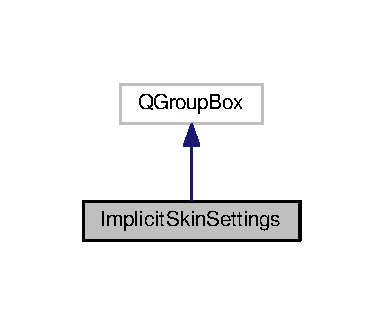
\includegraphics[width=184pt]{d0/ddd/classImplicitSkinSettings__inherit__graph}
\end{center}
\end{figure}


Collaboration diagram for Implicit\+Skin\+Settings\+:
\nopagebreak
\begin{figure}[H]
\begin{center}
\leavevmode
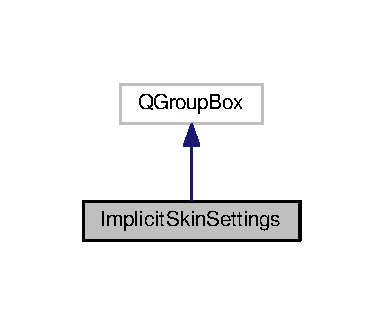
\includegraphics[width=184pt]{d2/d88/classImplicitSkinSettings__coll__graph}
\end{center}
\end{figure}
\subsection*{Signals}
\begin{DoxyCompactItemize}
\item 
void \hyperlink{classImplicitSkinSettings_a4a30d8a8ad0975689931556565c70762}{Iterations\+Changed} (int iterations)\hypertarget{classImplicitSkinSettings_a4a30d8a8ad0975689931556565c70762}{}\label{classImplicitSkinSettings_a4a30d8a8ad0975689931556565c70762}

\begin{DoxyCompactList}\small\item\em Qt Signal emitted when iteration changed. \end{DoxyCompactList}\item 
void \hyperlink{classImplicitSkinSettings_acc0660b7e87c960f9673e00ac7a5e781}{Sigma\+Changed} (float sigma)\hypertarget{classImplicitSkinSettings_acc0660b7e87c960f9673e00ac7a5e781}{}\label{classImplicitSkinSettings_acc0660b7e87c960f9673e00ac7a5e781}

\begin{DoxyCompactList}\small\item\em Qt Signal emitted when sigma chanegd. \end{DoxyCompactList}\item 
void \hyperlink{classImplicitSkinSettings_aaaa5d6d175fd2c6ffb7a6e5cec53d457}{Contact\+Angle\+Changed} (float contact\+Angle)\hypertarget{classImplicitSkinSettings_aaaa5d6d175fd2c6ffb7a6e5cec53d457}{}\label{classImplicitSkinSettings_aaaa5d6d175fd2c6ffb7a6e5cec53d457}

\begin{DoxyCompactList}\small\item\em Qt Signal emitted when contact angle changed. \end{DoxyCompactList}\item 
void \hyperlink{classImplicitSkinSettings_a874064fa151df9adf093561fb09b7fa4}{Load\+Animation\+Clicked} ()\hypertarget{classImplicitSkinSettings_a874064fa151df9adf093561fb09b7fa4}{}\label{classImplicitSkinSettings_a874064fa151df9adf093561fb09b7fa4}

\begin{DoxyCompactList}\small\item\em Qt Signal emitted when load animation button clicked. \end{DoxyCompactList}\item 
void \hyperlink{classImplicitSkinSettings_a6c25ea84730485ab8cc07e13b1f9e14c}{Browse\+Animation\+Clicked} ()\hypertarget{classImplicitSkinSettings_a6c25ea84730485ab8cc07e13b1f9e14c}{}\label{classImplicitSkinSettings_a6c25ea84730485ab8cc07e13b1f9e14c}

\begin{DoxyCompactList}\small\item\em Qt Signal emitted when browse animation button clicked. \end{DoxyCompactList}\item 
void \hyperlink{classImplicitSkinSettings_abc1b379dc1c51a8ca631edda32706df3}{Animation\+File\+Chnaged} (std\+::string file)\hypertarget{classImplicitSkinSettings_abc1b379dc1c51a8ca631edda32706df3}{}\label{classImplicitSkinSettings_abc1b379dc1c51a8ca631edda32706df3}

\begin{DoxyCompactList}\small\item\em Qt Signal emitted when animation file name changed. \end{DoxyCompactList}\item 
void {\bfseries Render\+Mesh\+Changed} (bool checked)\hypertarget{classImplicitSkinSettings_aecbd4de73c7fe10b4bb60896c3d67c25}{}\label{classImplicitSkinSettings_aecbd4de73c7fe10b4bb60896c3d67c25}

\item 
void {\bfseries Wireframe\+Changed} (bool checked)\hypertarget{classImplicitSkinSettings_ad361ec65cf91284de54a5563ec7aadad}{}\label{classImplicitSkinSettings_ad361ec65cf91284de54a5563ec7aadad}

\item 
void {\bfseries Iso\+Surface\+Changed} (bool checked)\hypertarget{classImplicitSkinSettings_a745a1b43caec64c5f5297511db6c4c45}{}\label{classImplicitSkinSettings_a745a1b43caec64c5f5297511db6c4c45}

\item 
void {\bfseries Implicit\+Skin\+Changed} (bool checked)\hypertarget{classImplicitSkinSettings_a0ea98811435c2c1f69d01d15f0df81e7}{}\label{classImplicitSkinSettings_a0ea98811435c2c1f69d01d15f0df81e7}

\item 
void {\bfseries L\+B\+W\+Skin\+Changed} (bool checked)\hypertarget{classImplicitSkinSettings_a4984d2e43a23a103f1401d2c8a62b159}{}\label{classImplicitSkinSettings_a4984d2e43a23a103f1401d2c8a62b159}

\end{DoxyCompactItemize}
\subsection*{Public Member Functions}
\begin{DoxyCompactItemize}
\item 
\hyperlink{classImplicitSkinSettings_af22531962948dfdad26d517d51a4c185}{Implicit\+Skin\+Settings} (Q\+Widget $\ast$parent=0)\hypertarget{classImplicitSkinSettings_af22531962948dfdad26d517d51a4c185}{}\label{classImplicitSkinSettings_af22531962948dfdad26d517d51a4c185}

\begin{DoxyCompactList}\small\item\em constructor \end{DoxyCompactList}\item 
\hyperlink{classImplicitSkinSettings_a905d9f0aa6a643620a103f22a6531a8b}{$\sim$\+Implicit\+Skin\+Settings} ()\hypertarget{classImplicitSkinSettings_a905d9f0aa6a643620a103f22a6531a8b}{}\label{classImplicitSkinSettings_a905d9f0aa6a643620a103f22a6531a8b}

\begin{DoxyCompactList}\small\item\em destructor \end{DoxyCompactList}\item 
std\+::string \hyperlink{classImplicitSkinSettings_aef60d6c0a02d006dcd3828219c080fa9}{Get\+Animation\+File} ()\hypertarget{classImplicitSkinSettings_aef60d6c0a02d006dcd3828219c080fa9}{}\label{classImplicitSkinSettings_aef60d6c0a02d006dcd3828219c080fa9}

\begin{DoxyCompactList}\small\item\em Method to get the animation file that has been selected. \end{DoxyCompactList}\item 
int \hyperlink{classImplicitSkinSettings_a10db3d39aab7ad1e39a296ef8ad4be2b}{Get\+Iterations} ()\hypertarget{classImplicitSkinSettings_a10db3d39aab7ad1e39a296ef8ad4be2b}{}\label{classImplicitSkinSettings_a10db3d39aab7ad1e39a296ef8ad4be2b}

\begin{DoxyCompactList}\small\item\em Method to get the number of iterations for implicit skinning. \end{DoxyCompactList}\item 
double \hyperlink{classImplicitSkinSettings_a14bff3b55c1ea2e97c96652c678e180f}{Get\+Sigma} ()\hypertarget{classImplicitSkinSettings_a14bff3b55c1ea2e97c96652c678e180f}{}\label{classImplicitSkinSettings_a14bff3b55c1ea2e97c96652c678e180f}

\begin{DoxyCompactList}\small\item\em Method to get the value of sigma for implicit skinning. \end{DoxyCompactList}\item 
double \hyperlink{classImplicitSkinSettings_a1799bcc571f95a97238a9530a54ed93b}{Get\+Contact\+Angle} ()\hypertarget{classImplicitSkinSettings_a1799bcc571f95a97238a9530a54ed93b}{}\label{classImplicitSkinSettings_a1799bcc571f95a97238a9530a54ed93b}

\begin{DoxyCompactList}\small\item\em Method to get the contact angle used for imiplicit skinning. \end{DoxyCompactList}\end{DoxyCompactItemize}


\subsection{Detailed Description}
This class inherits from Q\+Group\+Box, it is a widget for selecting an animation file to load as well as editing settings for implicit skinning. 

\begin{DoxyAuthor}{Author}
Idris Miles 
\end{DoxyAuthor}
\begin{DoxyVersion}{Version}
1.\+0 
\end{DoxyVersion}
\begin{DoxyDate}{Date}
18/04/2017 
\end{DoxyDate}


The documentation for this class was generated from the following files\+:\begin{DoxyCompactItemize}
\item 
include/\+G\+U\+I/implicitskinsettings.\+h\item 
src/\+G\+U\+I/implicitskinsettings.\+cpp\end{DoxyCompactItemize}

\hypertarget{classUi_1_1ImplicitSkinSettings}{}\section{Ui\+:\+:Implicit\+Skin\+Settings Class Reference}
\label{classUi_1_1ImplicitSkinSettings}\index{Ui\+::\+Implicit\+Skin\+Settings@{Ui\+::\+Implicit\+Skin\+Settings}}


Inheritance diagram for Ui\+:\+:Implicit\+Skin\+Settings\+:\nopagebreak
\begin{figure}[H]
\begin{center}
\leavevmode
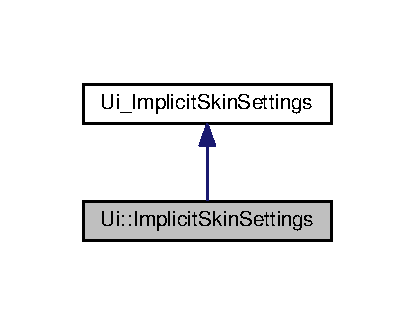
\includegraphics[width=199pt]{d5/df1/classUi_1_1ImplicitSkinSettings__inherit__graph}
\end{center}
\end{figure}


Collaboration diagram for Ui\+:\+:Implicit\+Skin\+Settings\+:\nopagebreak
\begin{figure}[H]
\begin{center}
\leavevmode
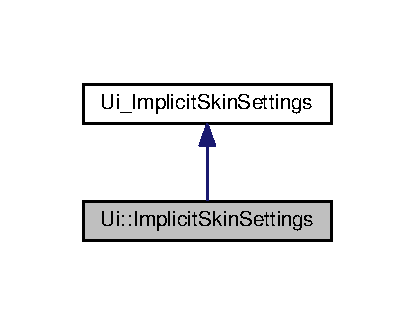
\includegraphics[width=199pt]{db/dc5/classUi_1_1ImplicitSkinSettings__coll__graph}
\end{center}
\end{figure}
\subsection*{Additional Inherited Members}


The documentation for this class was generated from the following file\+:\begin{DoxyCompactItemize}
\item 
ui/ui\+\_\+implicitskinsettings.\+h\end{DoxyCompactItemize}

\hypertarget{classMachingCube}{}\section{Maching\+Cube Class Reference}
\label{classMachingCube}\index{Maching\+Cube@{Maching\+Cube}}


basic maching cube algorithm  


\subsection*{Public Member Functions}
\begin{DoxyCompactItemize}
\item 
\hyperlink{classMachingCube_a47dca85496623aab6ee3ff0913db7d31}{Maching\+Cube} ()\hypertarget{classMachingCube_a47dca85496623aab6ee3ff0913db7d31}{}\label{classMachingCube_a47dca85496623aab6ee3ff0913db7d31}

\begin{DoxyCompactList}\small\item\em default constructor \end{DoxyCompactList}\item 
\hyperlink{classMachingCube_ab5b708b039b62182c2dc526a6ac6a181}{$\sim$\+Maching\+Cube} ()\hypertarget{classMachingCube_ab5b708b039b62182c2dc526a6ac6a181}{}\label{classMachingCube_ab5b708b039b62182c2dc526a6ac6a181}

\begin{DoxyCompactList}\small\item\em default destructor \end{DoxyCompactList}\end{DoxyCompactItemize}
\subsection*{Static Public Member Functions}
\begin{DoxyCompactItemize}
\item 
static void \hyperlink{classMachingCube_a5d38039696b93a4d555be3a2a49f684f}{Polygonize} (std\+::vector$<$ glm\+::vec3 $>$ \&\+\_\+verts, std\+::vector$<$ glm\+::vec3 $>$ \&\+\_\+norms, float $\ast$\+\_\+volume\+Data, const float \&\+\_\+isolevel, const int \&\+\_\+w, const int \&\+\_\+h, const int \&\+\_\+d, const float \&\+\_\+voxelW=1.\+0f, const float \&\+\_\+voxel\+H=1.\+0f, const float \&\+\_\+voxel\+D=1.\+0f)\hypertarget{classMachingCube_a5d38039696b93a4d555be3a2a49f684f}{}\label{classMachingCube_a5d38039696b93a4d555be3a2a49f684f}

\begin{DoxyCompactList}\small\item\em polygonize the iso surface \end{DoxyCompactList}\end{DoxyCompactItemize}
\subsection*{Static Protected Member Functions}
\begin{DoxyCompactItemize}
\item 
static void \hyperlink{classMachingCube_a03fe138d339db08d8f8deec1adb9eaef}{create\+Verts} (std\+::vector$<$ glm\+::vec3 $>$ \&\+\_\+verts, std\+::vector$<$ glm\+::vec3 $>$ \&\+\_\+norms, float $\ast$\+\_\+volume\+Data, const float \&\+\_\+isolevel, const int \&\+\_\+w, const int \&\+\_\+h, const int \&\+\_\+d, const float \&\+\_\+voxelW, const float \&\+\_\+voxelH, const float \&\+\_\+voxelD)\hypertarget{classMachingCube_a03fe138d339db08d8f8deec1adb9eaef}{}\label{classMachingCube_a03fe138d339db08d8f8deec1adb9eaef}

\begin{DoxyCompactList}\small\item\em Generate vertices and normals. \end{DoxyCompactList}\item 
static unsigned int \hyperlink{classMachingCube_a7a07c3e38877815f4bbe3d010b869e5c}{Maching\+Triangles} (\hyperlink{structVoxel}{Voxel} g, float iso, std\+::vector$<$ \hyperlink{structTriangle}{Triangle} $>$ \&tri\+List)\hypertarget{classMachingCube_a7a07c3e38877815f4bbe3d010b869e5c}{}\label{classMachingCube_a7a07c3e38877815f4bbe3d010b869e5c}

\begin{DoxyCompactList}\small\item\em extract triangles from each voxel, add the triangles into tri vector \end{DoxyCompactList}\item 
static glm\+::vec3 \hyperlink{classMachingCube_a09743e696d8b28797bafbfdb55df415c}{Vertex\+Interp} (float isolevel, glm\+::vec3 p1, glm\+::vec3 p2, float valp1, float valp2)\hypertarget{classMachingCube_a09743e696d8b28797bafbfdb55df415c}{}\label{classMachingCube_a09743e696d8b28797bafbfdb55df415c}

\begin{DoxyCompactList}\small\item\em intepolate the intersection point from the level value \end{DoxyCompactList}\item 
static glm\+::vec3 \hyperlink{classMachingCube_a96ce7dcf9383947e09c9bcb61302f2f7}{compute\+Triangle\+Normal} (\hyperlink{structTriangle}{Triangle} \&itr)\hypertarget{classMachingCube_a96ce7dcf9383947e09c9bcb61302f2f7}{}\label{classMachingCube_a96ce7dcf9383947e09c9bcb61302f2f7}

\begin{DoxyCompactList}\small\item\em compute the normal from the three vertices \end{DoxyCompactList}\end{DoxyCompactItemize}


\subsection{Detailed Description}
basic maching cube algorithm 

\begin{DoxyAuthor}{Author}
Xiaosong Yang, Idris Miles 
\end{DoxyAuthor}
\begin{DoxyVersion}{Version}
1.\+0 
\end{DoxyVersion}
\begin{DoxyDate}{Date}
14/01/13, 18/04/2017 
\end{DoxyDate}


The documentation for this class was generated from the following files\+:\begin{DoxyCompactItemize}
\item 
include/\+Machingcube/Maching\+Cube.\+h\item 
src/\+Machingcube/\hyperlink{MachingCube_8cpp}{Maching\+Cube.\+cpp}\end{DoxyCompactItemize}

\hypertarget{classMainWindow}{}\section{Main\+Window Class Reference}
\label{classMainWindow}\index{Main\+Window@{Main\+Window}}


Inheritance diagram for Main\+Window\+:\nopagebreak
\begin{figure}[H]
\begin{center}
\leavevmode
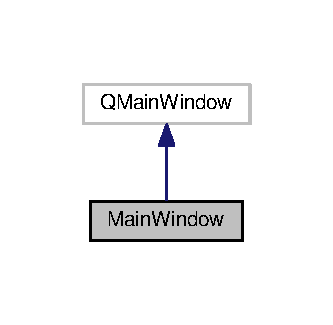
\includegraphics[width=160pt]{d1/d96/classMainWindow__inherit__graph}
\end{center}
\end{figure}


Collaboration diagram for Main\+Window\+:\nopagebreak
\begin{figure}[H]
\begin{center}
\leavevmode
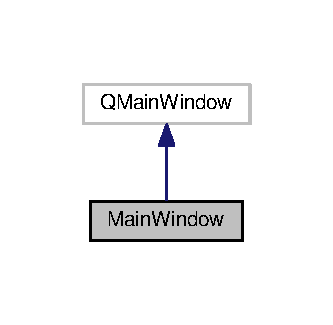
\includegraphics[width=160pt]{d2/d38/classMainWindow__coll__graph}
\end{center}
\end{figure}
\subsection*{Public Slots}
\begin{DoxyCompactItemize}
\item 
void {\bfseries Load\+Model} ()\hypertarget{classMainWindow_a43a9a9539c2ad020e510da06a2a8bfb7}{}\label{classMainWindow_a43a9a9539c2ad020e510da06a2a8bfb7}

\end{DoxyCompactItemize}
\subsection*{Public Member Functions}
\begin{DoxyCompactItemize}
\item 
{\bfseries Main\+Window} (Q\+Widget $\ast$parent=0)\hypertarget{classMainWindow_a8b244be8b7b7db1b08de2a2acb9409db}{}\label{classMainWindow_a8b244be8b7b7db1b08de2a2acb9409db}

\end{DoxyCompactItemize}


The documentation for this class was generated from the following files\+:\begin{DoxyCompactItemize}
\item 
include/mainwindow.\+h\item 
src/mainwindow.\+cpp\end{DoxyCompactItemize}

\hypertarget{classUi_1_1MainWindow}{}\section{Ui\+:\+:Main\+Window Class Reference}
\label{classUi_1_1MainWindow}\index{Ui\+::\+Main\+Window@{Ui\+::\+Main\+Window}}


Inheritance diagram for Ui\+:\+:Main\+Window\+:\nopagebreak
\begin{figure}[H]
\begin{center}
\leavevmode
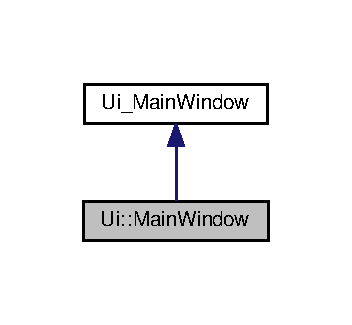
\includegraphics[width=169pt]{d5/db9/classUi_1_1MainWindow__inherit__graph}
\end{center}
\end{figure}


Collaboration diagram for Ui\+:\+:Main\+Window\+:
\nopagebreak
\begin{figure}[H]
\begin{center}
\leavevmode
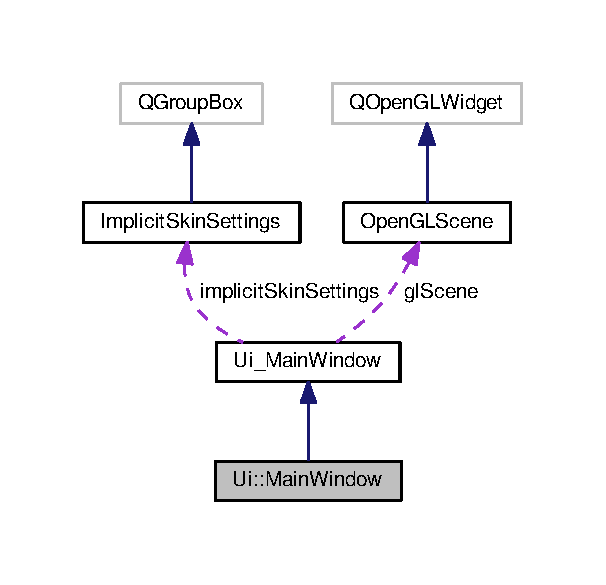
\includegraphics[width=291pt]{d2/db6/classUi_1_1MainWindow__coll__graph}
\end{center}
\end{figure}
\subsection*{Additional Inherited Members}


The documentation for this class was generated from the following file\+:\begin{DoxyCompactItemize}
\item 
ui/ui\+\_\+mainwindow.\+h\end{DoxyCompactItemize}

\hypertarget{classMesh}{}\section{Mesh Class Reference}
\label{classMesh}\index{Mesh@{Mesh}}


\hyperlink{classMesh}{Mesh} data structure, holds vertices, triangle indices, normals, vertex colours, mesh colour, vertex U\+Vs, vertex bone weights (for skinning).  




{\ttfamily \#include $<$mesh.\+h$>$}

\subsection*{Public Member Functions}
\begin{DoxyCompactItemize}
\item 
\hyperlink{classMesh_a2af137f1571af89172b9c102302c416b}{Mesh} ()\hypertarget{classMesh_a2af137f1571af89172b9c102302c416b}{}\label{classMesh_a2af137f1571af89172b9c102302c416b}

\begin{DoxyCompactList}\small\item\em constructor \end{DoxyCompactList}\item 
bool \hyperlink{classMesh_a933629b3306bc2fe4a7b6e9eaaecdd06}{Get\+One\+Ring\+Neighours} (std\+::vector$<$ std\+::vector$<$ int $>$$>$ \&\+\_\+one\+Ring) const 
\begin{DoxyCompactList}\small\item\em Method to get the one ring neighbourhoods. \end{DoxyCompactList}\item 
void \hyperlink{classMesh_a9228b41d6b37367e655b6fd5e719c42f}{Compute\+One\+Ring} ()\hypertarget{classMesh_a9228b41d6b37367e655b6fd5e719c42f}{}\label{classMesh_a9228b41d6b37367e655b6fd5e719c42f}

\begin{DoxyCompactList}\small\item\em Method to compute the one ring neighbourhood. \end{DoxyCompactList}\item 
void \hyperlink{classMesh_a9f8c0578b4a766b0e3cbe3df5fe42311}{Compute\+B\+Box} (const bool \&\+\_\+recompute=false)
\begin{DoxyCompactList}\small\item\em Method to internally compute the axis aligned bounding box of this mesh. \end{DoxyCompactList}\end{DoxyCompactItemize}
\subsection*{Public Attributes}
\begin{DoxyCompactItemize}
\item 
std\+::vector$<$ glm\+::vec3 $>$ \hyperlink{classMesh_aa409beb8a6df4709baf7b47beac9581d}{m\+\_\+mesh\+Verts}\hypertarget{classMesh_aa409beb8a6df4709baf7b47beac9581d}{}\label{classMesh_aa409beb8a6df4709baf7b47beac9581d}

\begin{DoxyCompactList}\small\item\em m\+\_\+mesh\+Verts, a vector containing all vertices of the mesh. \end{DoxyCompactList}\item 
std\+::vector$<$ glm\+::vec3 $>$ \hyperlink{classMesh_afdd4c5d1d7e19176a1919cc6890db137}{m\+\_\+mesh\+Norms}\hypertarget{classMesh_afdd4c5d1d7e19176a1919cc6890db137}{}\label{classMesh_afdd4c5d1d7e19176a1919cc6890db137}

\begin{DoxyCompactList}\small\item\em m\+\_\+mesh\+Norms, a vector containing all normals of the mesh. \end{DoxyCompactList}\item 
std\+::vector$<$ glm\+::ivec3 $>$ \hyperlink{classMesh_ab69b200bd81cee173a6226b290c5e3a6}{m\+\_\+mesh\+Tris}\hypertarget{classMesh_ab69b200bd81cee173a6226b290c5e3a6}{}\label{classMesh_ab69b200bd81cee173a6226b290c5e3a6}

\begin{DoxyCompactList}\small\item\em m\+\_\+mesh\+Tris, a vector containing all the triangle indices of the mesh. \end{DoxyCompactList}\item 
std\+::vector$<$ \hyperlink{structVertexBoneData}{Vertex\+Bone\+Data} $>$ \hyperlink{classMesh_aa7d497de323ddfe418e4b8cf5ee9d549}{m\+\_\+mesh\+Bone\+Weights}\hypertarget{classMesh_aa7d497de323ddfe418e4b8cf5ee9d549}{}\label{classMesh_aa7d497de323ddfe418e4b8cf5ee9d549}

\begin{DoxyCompactList}\small\item\em m\+\_\+mesh\+Bone\+Weights, a vector containing all the vertices bone weight data. \end{DoxyCompactList}\item 
std\+::vector$<$ glm\+::vec3 $>$ \hyperlink{classMesh_a0ef923278d71ec31675d8bc2c16e2ab5}{m\+\_\+mesh\+Vert\+Colours}\hypertarget{classMesh_a0ef923278d71ec31675d8bc2c16e2ab5}{}\label{classMesh_a0ef923278d71ec31675d8bc2c16e2ab5}

\begin{DoxyCompactList}\small\item\em m\+\_\+mesh\+Vert\+Colours, a vector containing all the vertex colours of the mesh. \end{DoxyCompactList}\item 
std\+::vector$<$ glm\+::vec2 $>$ \hyperlink{classMesh_af7ceb87d2dcde9aff06e0b986de9640e}{m\+\_\+mesh\+U\+Vs}\hypertarget{classMesh_af7ceb87d2dcde9aff06e0b986de9640e}{}\label{classMesh_af7ceb87d2dcde9aff06e0b986de9640e}

\begin{DoxyCompactList}\small\item\em m\+\_\+mesh\+U\+Vs, a vector containing all the vertex UV\textquotesingle{}s of the mesh. \end{DoxyCompactList}\item 
glm\+::vec3 \hyperlink{classMesh_a4778512cc7163a50aad277ff4f6b8ec8}{m\+\_\+colour}\hypertarget{classMesh_a4778512cc7163a50aad277ff4f6b8ec8}{}\label{classMesh_a4778512cc7163a50aad277ff4f6b8ec8}

\begin{DoxyCompactList}\small\item\em m\+\_\+colour, a base colour of the whole mesh, used for simple rendering. \end{DoxyCompactList}\item 
std\+::vector$<$ std\+::vector$<$ int $>$ $>$ \hyperlink{classMesh_a80d54fe600d1a19d40315d6f0d4d42f1}{m\+\_\+mesh\+Verts\+One\+Ring}\hypertarget{classMesh_a80d54fe600d1a19d40315d6f0d4d42f1}{}\label{classMesh_a80d54fe600d1a19d40315d6f0d4d42f1}

\begin{DoxyCompactList}\small\item\em m\+\_\+mesh\+Verts\+One\+Ring, the one ring neighbourhood for each vertex by id \end{DoxyCompactList}\item 
glm\+::vec3 \hyperlink{classMesh_a4d45309b6e6500312ebfc4e9ac44a477}{m\+\_\+min\+B\+Box}\hypertarget{classMesh_a4d45309b6e6500312ebfc4e9ac44a477}{}\label{classMesh_a4d45309b6e6500312ebfc4e9ac44a477}

\begin{DoxyCompactList}\small\item\em m\+\_\+min\+B\+Box, the min half of the axis aligned bounding box \end{DoxyCompactList}\item 
glm\+::vec3 \hyperlink{classMesh_ad6f161331138fbf12fce54efd5c0a212}{m\+\_\+max\+B\+Box}\hypertarget{classMesh_ad6f161331138fbf12fce54efd5c0a212}{}\label{classMesh_ad6f161331138fbf12fce54efd5c0a212}

\begin{DoxyCompactList}\small\item\em m\+\_\+max\+B\+Box, the max half of the axis aligned bounding box \end{DoxyCompactList}\end{DoxyCompactItemize}


\subsection{Detailed Description}
\hyperlink{classMesh}{Mesh} data structure, holds vertices, triangle indices, normals, vertex colours, mesh colour, vertex U\+Vs, vertex bone weights (for skinning). 

\subsection{Member Function Documentation}
\index{Mesh@{Mesh}!Compute\+B\+Box@{Compute\+B\+Box}}
\index{Compute\+B\+Box@{Compute\+B\+Box}!Mesh@{Mesh}}
\subsubsection[{\texorpdfstring{Compute\+B\+Box(const bool \&\+\_\+recompute=false)}{ComputeBBox(const bool &_recompute=false)}}]{\setlength{\rightskip}{0pt plus 5cm}void Mesh\+::\+Compute\+B\+Box (
\begin{DoxyParamCaption}
\item[{const bool \&}]{\+\_\+recompute = {\ttfamily false}}
\end{DoxyParamCaption}
)\hspace{0.3cm}{\ttfamily [inline]}}\hypertarget{classMesh_a9f8c0578b4a766b0e3cbe3df5fe42311}{}\label{classMesh_a9f8c0578b4a766b0e3cbe3df5fe42311}


Method to internally compute the axis aligned bounding box of this mesh. 


\begin{DoxyParams}{Parameters}
{\em \+\_\+recompute} & \+: boolean to recompute this if it has previously been computed but the mesh may have changed since \\
\hline
\end{DoxyParams}
\index{Mesh@{Mesh}!Get\+One\+Ring\+Neighours@{Get\+One\+Ring\+Neighours}}
\index{Get\+One\+Ring\+Neighours@{Get\+One\+Ring\+Neighours}!Mesh@{Mesh}}
\subsubsection[{\texorpdfstring{Get\+One\+Ring\+Neighours(std\+::vector$<$ std\+::vector$<$ int $>$$>$ \&\+\_\+one\+Ring) const }{GetOneRingNeighours(std::vector< std::vector< int >> &_oneRing) const }}]{\setlength{\rightskip}{0pt plus 5cm}bool Mesh\+::\+Get\+One\+Ring\+Neighours (
\begin{DoxyParamCaption}
\item[{std\+::vector$<$ std\+::vector$<$ int $>$$>$ \&}]{\+\_\+one\+Ring}
\end{DoxyParamCaption}
) const\hspace{0.3cm}{\ttfamily [inline]}}\hypertarget{classMesh_a933629b3306bc2fe4a7b6e9eaaecdd06}{}\label{classMesh_a933629b3306bc2fe4a7b6e9eaaecdd06}


Method to get the one ring neighbourhoods. 


\begin{DoxyParams}{Parameters}
{\em \+\_\+one\+Ring} & \+: This is a vector of vectors of ints and holds the one ring neighbourhood for each vertex by their Id \\
\hline
\end{DoxyParams}


The documentation for this class was generated from the following file\+:\begin{DoxyCompactItemize}
\item 
include/mesh.\+h\end{DoxyCompactItemize}

\hypertarget{classModel}{}\section{Model Class Reference}
\label{classModel}\index{Model@{Model}}


A model, this holds the mesh, animated rig, and skin deformer, it also handles the rendering of itself.  




{\ttfamily \#include $<$model.\+h$>$}

\subsection*{Public Member Functions}
\begin{DoxyCompactItemize}
\item 
\hyperlink{classModel_ae3b375de5f6df4faf74a95d64748e048}{Model} ()\hypertarget{classModel_ae3b375de5f6df4faf74a95d64748e048}{}\label{classModel_ae3b375de5f6df4faf74a95d64748e048}

\begin{DoxyCompactList}\small\item\em constructor \end{DoxyCompactList}\item 
\hyperlink{classModel_ad6ebd2062a0b823db841a0b88baac4c0}{$\sim$\+Model} ()\hypertarget{classModel_ad6ebd2062a0b823db841a0b88baac4c0}{}\label{classModel_ad6ebd2062a0b823db841a0b88baac4c0}

\begin{DoxyCompactList}\small\item\em destructor \end{DoxyCompactList}\item 
void \hyperlink{classModel_a9fc27c23ef71e81fc9949953125fcee8}{Initialise} ()\hypertarget{classModel_a9fc27c23ef71e81fc9949953125fcee8}{}\label{classModel_a9fc27c23ef71e81fc9949953125fcee8}

\begin{DoxyCompactList}\small\item\em Method to initialise model. \end{DoxyCompactList}\item 
void \hyperlink{classModel_ac02a26d23143d6456a726957e1042840}{Draw\+Mesh} ()\hypertarget{classModel_ac02a26d23143d6456a726957e1042840}{}\label{classModel_ac02a26d23143d6456a726957e1042840}

\begin{DoxyCompactList}\small\item\em Method to draw the skinned animated model. \end{DoxyCompactList}\item 
void \hyperlink{classModel_a593d18e249b56ca87fdc6339916e7b5e}{Draw\+Rig} ()\hypertarget{classModel_a593d18e249b56ca87fdc6339916e7b5e}{}\label{classModel_a593d18e249b56ca87fdc6339916e7b5e}

\begin{DoxyCompactList}\small\item\em Method to draw the animated rig. \end{DoxyCompactList}\item 
void \hyperlink{classModel_a72cc0344f05776e6bbbb9ec82ed0b7b6}{Animate} (const float \+\_\+animation\+Time)
\begin{DoxyCompactList}\small\item\em Method to animate the model. \end{DoxyCompactList}\item 
void \hyperlink{classModel_ad8697962971f8443f3e1bfd474e6ac20}{Toggle\+Wireframe} ()\hypertarget{classModel_ad8697962971f8443f3e1bfd474e6ac20}{}\label{classModel_ad8697962971f8443f3e1bfd474e6ac20}

\begin{DoxyCompactList}\small\item\em Method to toggle rendering the skinned mesh in wireframe or filled. \end{DoxyCompactList}\item 
void \hyperlink{classModel_a7ce564f5eb3e962970bc285305a352f7}{Toggle\+Skinned\+Surface} ()\hypertarget{classModel_a7ce564f5eb3e962970bc285305a352f7}{}\label{classModel_a7ce564f5eb3e962970bc285305a352f7}

\begin{DoxyCompactList}\small\item\em Method to toggle rendering of the skinned mesh. \end{DoxyCompactList}\item 
void \hyperlink{classModel_ad453680f0603420e226c2aa4a74db9dd}{Toggle\+Skinned\+Implicit\+Surface} ()\hypertarget{classModel_ad453680f0603420e226c2aa4a74db9dd}{}\label{classModel_ad453680f0603420e226c2aa4a74db9dd}

\begin{DoxyCompactList}\small\item\em Method to toggle performing implicit or linear blend weight skinning. \end{DoxyCompactList}\item 
void \hyperlink{classModel_ac97e2c6ccbe0937d0c7b5aed1bfceb04}{Toggle\+Iso\+Surface} ()\hypertarget{classModel_ac97e2c6ccbe0937d0c7b5aed1bfceb04}{}\label{classModel_ac97e2c6ccbe0937d0c7b5aed1bfceb04}

\begin{DoxyCompactList}\small\item\em Method to toggle rendering the iso surface of the global field from the implicit deformer. \end{DoxyCompactList}\item 
void \hyperlink{classModel_afad9aa7af2bdbdf511dcd3e0748a2d9a}{Set\+Light\+Pos} (const glm\+::vec3 \&\+\_\+light\+Pos)\hypertarget{classModel_afad9aa7af2bdbdf511dcd3e0748a2d9a}{}\label{classModel_afad9aa7af2bdbdf511dcd3e0748a2d9a}

\begin{DoxyCompactList}\small\item\em Method to set light position. \end{DoxyCompactList}\item 
void \hyperlink{classModel_a88d681e1ea367b0140b04ae84ee72512}{Set\+Model\+Matrix} (const glm\+::mat4 \&\+\_\+model\+Mat)\hypertarget{classModel_a88d681e1ea367b0140b04ae84ee72512}{}\label{classModel_a88d681e1ea367b0140b04ae84ee72512}

\begin{DoxyCompactList}\small\item\em Method to set the model matrix. \end{DoxyCompactList}\item 
void \hyperlink{classModel_a8cffd0fa41ec392fabaa02fce9f2624e}{Set\+Normal\+Matrix} (const glm\+::mat3 \&\+\_\+norm\+Mat)\hypertarget{classModel_a8cffd0fa41ec392fabaa02fce9f2624e}{}\label{classModel_a8cffd0fa41ec392fabaa02fce9f2624e}

\begin{DoxyCompactList}\small\item\em Method to set the normal matrix. \end{DoxyCompactList}\item 
void \hyperlink{classModel_aa98bb18be5df8aef0da8aa47d6e09f19}{Set\+View\+Matrix} (const glm\+::mat4 \&\+\_\+view\+Mat)\hypertarget{classModel_aa98bb18be5df8aef0da8aa47d6e09f19}{}\label{classModel_aa98bb18be5df8aef0da8aa47d6e09f19}

\begin{DoxyCompactList}\small\item\em Method to set the view matrix. \end{DoxyCompactList}\item 
void \hyperlink{classModel_aee6397055a5aa1e964cde1639da05122}{Set\+Projection\+Matrix} (const glm\+::mat4 \&\+\_\+proj\+Mat)\hypertarget{classModel_aee6397055a5aa1e964cde1639da05122}{}\label{classModel_aee6397055a5aa1e964cde1639da05122}

\begin{DoxyCompactList}\small\item\em Method to set the projection matrix. \end{DoxyCompactList}\item 
\hyperlink{classRig}{Rig} \& \hyperlink{classModel_ab41210858b52e222212ec2c9e4bfbed1}{Get\+Rig} ()\hypertarget{classModel_ab41210858b52e222212ec2c9e4bfbed1}{}\label{classModel_ab41210858b52e222212ec2c9e4bfbed1}

\begin{DoxyCompactList}\small\item\em Method to get the \hyperlink{classRig}{Rig}. \end{DoxyCompactList}\item 
\hyperlink{classMesh}{Mesh} \& \hyperlink{classModel_a868b3918a895ab46d6b7f9fdd74106ac}{Get\+Mesh} ()\hypertarget{classModel_a868b3918a895ab46d6b7f9fdd74106ac}{}\label{classModel_a868b3918a895ab46d6b7f9fdd74106ac}

\begin{DoxyCompactList}\small\item\em Method to get the model mesh. \end{DoxyCompactList}\item 
\hyperlink{classMesh}{Mesh} \& \hyperlink{classModel_a14500b0c2d22f4cf8b823a217900e85a}{Get\+Rig\+Mesh} ()\hypertarget{classModel_a14500b0c2d22f4cf8b823a217900e85a}{}\label{classModel_a14500b0c2d22f4cf8b823a217900e85a}

\begin{DoxyCompactList}\small\item\em Method to get the \hyperlink{classRig}{Rig} \hyperlink{classMesh}{Mesh}. \end{DoxyCompactList}\end{DoxyCompactItemize}


\subsection{Detailed Description}
A model, this holds the mesh, animated rig, and skin deformer, it also handles the rendering of itself. 

\subsection{Member Function Documentation}
\index{Model@{Model}!Animate@{Animate}}
\index{Animate@{Animate}!Model@{Model}}
\subsubsection[{\texorpdfstring{Animate(const float \+\_\+animation\+Time)}{Animate(const float _animationTime)}}]{\setlength{\rightskip}{0pt plus 5cm}void Model\+::\+Animate (
\begin{DoxyParamCaption}
\item[{const float}]{\+\_\+animation\+Time}
\end{DoxyParamCaption}
)}\hypertarget{classModel_a72cc0344f05776e6bbbb9ec82ed0b7b6}{}\label{classModel_a72cc0344f05776e6bbbb9ec82ed0b7b6}


Method to animate the model. 


\begin{DoxyParams}{Parameters}
{\em \+\_\+animation\+Time} & \+: the time the animation should be a \\
\hline
\end{DoxyParams}


The documentation for this class was generated from the following files\+:\begin{DoxyCompactItemize}
\item 
include/model.\+h\item 
src/model.\+cpp\end{DoxyCompactItemize}

\hypertarget{classModelLoader}{}\section{Model\+Loader Class Reference}
\label{classModelLoader}\index{Model\+Loader@{Model\+Loader}}


This class loades a model from file.  




{\ttfamily \#include $<$modelloader.\+h$>$}

\subsection*{Public Member Functions}
\begin{DoxyCompactItemize}
\item 
\hyperlink{classModelLoader_a5892e5788d106f1e57124a73cdb2ddb5}{Model\+Loader} ()\hypertarget{classModelLoader_a5892e5788d106f1e57124a73cdb2ddb5}{}\label{classModelLoader_a5892e5788d106f1e57124a73cdb2ddb5}

\begin{DoxyCompactList}\small\item\em constructor \end{DoxyCompactList}\end{DoxyCompactItemize}
\subsection*{Static Public Member Functions}
\begin{DoxyCompactItemize}
\item 
static \hyperlink{classModel}{Model} $\ast$ \hyperlink{classModelLoader_ab89c5571cb8711db7d0c4aff88884544}{Load\+Model} (const std\+::string \&\+\_\+file)
\begin{DoxyCompactList}\small\item\em Method to load a new model from file. \end{DoxyCompactList}\end{DoxyCompactItemize}


\subsection{Detailed Description}
This class loades a model from file. 

\begin{DoxyAuthor}{Author}
Idris Miles 
\end{DoxyAuthor}
\begin{DoxyVersion}{Version}
1.\+0 
\end{DoxyVersion}
\begin{DoxyDate}{Date}
18/04/2017 
\end{DoxyDate}


\subsection{Member Function Documentation}
\index{Model\+Loader@{Model\+Loader}!Load\+Model@{Load\+Model}}
\index{Load\+Model@{Load\+Model}!Model\+Loader@{Model\+Loader}}
\subsubsection[{\texorpdfstring{Load\+Model(const std\+::string \&\+\_\+file)}{LoadModel(const std::string &_file)}}]{\setlength{\rightskip}{0pt plus 5cm}{\bf Model} $\ast$ Model\+Loader\+::\+Load\+Model (
\begin{DoxyParamCaption}
\item[{const std\+::string \&}]{\+\_\+file}
\end{DoxyParamCaption}
)\hspace{0.3cm}{\ttfamily [static]}}\hypertarget{classModelLoader_ab89c5571cb8711db7d0c4aff88884544}{}\label{classModelLoader_ab89c5571cb8711db7d0c4aff88884544}


Method to load a new model from file. 


\begin{DoxyParams}{Parameters}
{\em \+\_\+file} & \+: file we wish to load \\
\hline
\end{DoxyParams}


The documentation for this class was generated from the following files\+:\begin{DoxyCompactItemize}
\item 
include/modelloader.\+h\item 
src/modelloader.\+cpp\end{DoxyCompactItemize}

\hypertarget{classOpenGLScene}{}\section{Open\+G\+L\+Scene Class Reference}
\label{classOpenGLScene}\index{Open\+G\+L\+Scene@{Open\+G\+L\+Scene}}


This class is iniherited from Q\+Open\+G\+L\+Widget and acts as our scene. This is based on \href{https://github.com/IdrisMiles/QtOpenGL}{\tt https\+://github.\+com/\+Idris\+Miles/\+Qt\+Open\+GL}.  




{\ttfamily \#include $<$openglscene.\+h$>$}



Inheritance diagram for Open\+G\+L\+Scene\+:\nopagebreak
\begin{figure}[H]
\begin{center}
\leavevmode
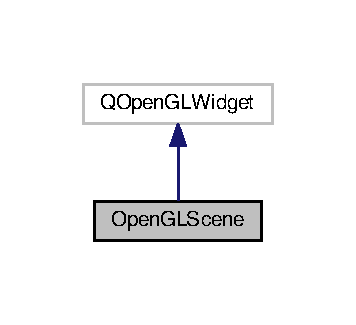
\includegraphics[width=171pt]{de/d3e/classOpenGLScene__inherit__graph}
\end{center}
\end{figure}


Collaboration diagram for Open\+G\+L\+Scene\+:\nopagebreak
\begin{figure}[H]
\begin{center}
\leavevmode
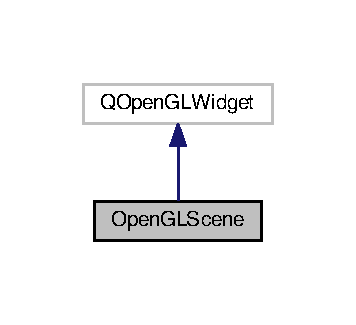
\includegraphics[width=171pt]{da/d38/classOpenGLScene__coll__graph}
\end{center}
\end{figure}
\subsection*{Public Slots}
\begin{DoxyCompactItemize}
\item 
void \hyperlink{classOpenGLScene_ac46ceeabc09c0773edaad6af67d6351b}{set\+X\+Rotation} (int angle)\hypertarget{classOpenGLScene_ac46ceeabc09c0773edaad6af67d6351b}{}\label{classOpenGLScene_ac46ceeabc09c0773edaad6af67d6351b}

\begin{DoxyCompactList}\small\item\em set X rotation of world \end{DoxyCompactList}\item 
void \hyperlink{classOpenGLScene_a842a2ecfc834e10f20bbfdaca361c690}{set\+Y\+Rotation} (int angle)\hypertarget{classOpenGLScene_a842a2ecfc834e10f20bbfdaca361c690}{}\label{classOpenGLScene_a842a2ecfc834e10f20bbfdaca361c690}

\begin{DoxyCompactList}\small\item\em set Y rotation of world \end{DoxyCompactList}\item 
void \hyperlink{classOpenGLScene_a6c67c7e3eb0e9c28e86575d4e208e6b7}{set\+Z\+Rotation} (int angle)\hypertarget{classOpenGLScene_a6c67c7e3eb0e9c28e86575d4e208e6b7}{}\label{classOpenGLScene_a6c67c7e3eb0e9c28e86575d4e208e6b7}

\begin{DoxyCompactList}\small\item\em set Z rotation of world \end{DoxyCompactList}\item 
void \hyperlink{classOpenGLScene_adc846d24b03db9b39852a03d87ef1155}{set\+X\+Translation} (int x)\hypertarget{classOpenGLScene_adc846d24b03db9b39852a03d87ef1155}{}\label{classOpenGLScene_adc846d24b03db9b39852a03d87ef1155}

\begin{DoxyCompactList}\small\item\em set X translation of world \end{DoxyCompactList}\item 
void \hyperlink{classOpenGLScene_a724dca13497de1e3ca8467aedab40fcf}{set\+Y\+Translation} (int y)\hypertarget{classOpenGLScene_a724dca13497de1e3ca8467aedab40fcf}{}\label{classOpenGLScene_a724dca13497de1e3ca8467aedab40fcf}

\begin{DoxyCompactList}\small\item\em set Y translation of world \end{DoxyCompactList}\item 
void \hyperlink{classOpenGLScene_a407be2074846dd3798e3e5cd84cc6673}{set\+Z\+Translation} (int z)\hypertarget{classOpenGLScene_a407be2074846dd3798e3e5cd84cc6673}{}\label{classOpenGLScene_a407be2074846dd3798e3e5cd84cc6673}

\begin{DoxyCompactList}\small\item\em set Z translation of world \end{DoxyCompactList}\item 
void \hyperlink{classOpenGLScene_a636436c84b2687666e87d5f1dbe43167}{cleanup} ()\hypertarget{classOpenGLScene_a636436c84b2687666e87d5f1dbe43167}{}\label{classOpenGLScene_a636436c84b2687666e87d5f1dbe43167}

\begin{DoxyCompactList}\small\item\em clean up scene \end{DoxyCompactList}\item 
void \hyperlink{classOpenGLScene_a02677ce16ce1344cbf75d1d394246653}{Update\+Anim} ()\hypertarget{classOpenGLScene_a02677ce16ce1344cbf75d1d394246653}{}\label{classOpenGLScene_a02677ce16ce1344cbf75d1d394246653}

\begin{DoxyCompactList}\small\item\em update animation of models \end{DoxyCompactList}\item 
void \hyperlink{classOpenGLScene_a96f0459efbbc6de5dbca69d1fb982b15}{Update\+Draw} ()\hypertarget{classOpenGLScene_a96f0459efbbc6de5dbca69d1fb982b15}{}\label{classOpenGLScene_a96f0459efbbc6de5dbca69d1fb982b15}

\begin{DoxyCompactList}\small\item\em calls update \end{DoxyCompactList}\end{DoxyCompactItemize}
\subsection*{Public Member Functions}
\begin{DoxyCompactItemize}
\item 
\hyperlink{classOpenGLScene_a22d3e62d9b562baf3f5cda3511a85578}{Open\+G\+L\+Scene} (Q\+Widget $\ast$parent=0)\hypertarget{classOpenGLScene_a22d3e62d9b562baf3f5cda3511a85578}{}\label{classOpenGLScene_a22d3e62d9b562baf3f5cda3511a85578}

\begin{DoxyCompactList}\small\item\em constructor \end{DoxyCompactList}\item 
\hyperlink{classOpenGLScene_a9e3b2533ed475dd7b7c103d5545c8636}{$\sim$\+Open\+G\+L\+Scene} ()\hypertarget{classOpenGLScene_a9e3b2533ed475dd7b7c103d5545c8636}{}\label{classOpenGLScene_a9e3b2533ed475dd7b7c103d5545c8636}

\begin{DoxyCompactList}\small\item\em destructor \end{DoxyCompactList}\item 
std\+::shared\+\_\+ptr$<$ \hyperlink{classModel}{Model} $>$ \hyperlink{classOpenGLScene_a0696eb5454ed88262869667fb3c49869}{Add\+Model} (const std\+::string \&\+\_\+model\+File)
\begin{DoxyCompactList}\small\item\em Method to add a model into the scene. \end{DoxyCompactList}\end{DoxyCompactItemize}
\subsection*{Protected Member Functions}
\begin{DoxyCompactItemize}
\item 
void \hyperlink{classOpenGLScene_af9736a6bf7ba52614c7953d4f4e1778c}{initialize\+GL} () Q\+\_\+\+D\+E\+C\+L\+\_\+\+O\+V\+E\+R\+R\+I\+DE\hypertarget{classOpenGLScene_af9736a6bf7ba52614c7953d4f4e1778c}{}\label{classOpenGLScene_af9736a6bf7ba52614c7953d4f4e1778c}

\begin{DoxyCompactList}\small\item\em overloaded method from Q\+Open\+G\+L\+Widget, initialises GL stuff and starts animation/drawing timers \end{DoxyCompactList}\item 
void \hyperlink{classOpenGLScene_a172bd568ea2ba8b18e94dc8c0640bacd}{paint\+GL} () Q\+\_\+\+D\+E\+C\+L\+\_\+\+O\+V\+E\+R\+R\+I\+DE\hypertarget{classOpenGLScene_a172bd568ea2ba8b18e94dc8c0640bacd}{}\label{classOpenGLScene_a172bd568ea2ba8b18e94dc8c0640bacd}

\begin{DoxyCompactList}\small\item\em overloaded method from Q\+Open\+G\+L\+Widget, draw our scene \end{DoxyCompactList}\item 
void \hyperlink{classOpenGLScene_ae1c824958ef867f3009b24e841ef5842}{resize\+GL} (int width, int height) Q\+\_\+\+D\+E\+C\+L\+\_\+\+O\+V\+E\+R\+R\+I\+DE\hypertarget{classOpenGLScene_ae1c824958ef867f3009b24e841ef5842}{}\label{classOpenGLScene_ae1c824958ef867f3009b24e841ef5842}

\begin{DoxyCompactList}\small\item\em overloaded method from Q\+Open\+G\+L\+Widget, updates projection matrix \end{DoxyCompactList}\item 
void \hyperlink{classOpenGLScene_aaf2d0276c9b09112edb1d830e4258b78}{mouse\+Press\+Event} (Q\+Mouse\+Event $\ast$event) Q\+\_\+\+D\+E\+C\+L\+\_\+\+O\+V\+E\+R\+R\+I\+DE\hypertarget{classOpenGLScene_aaf2d0276c9b09112edb1d830e4258b78}{}\label{classOpenGLScene_aaf2d0276c9b09112edb1d830e4258b78}

\begin{DoxyCompactList}\small\item\em overloaded method from Q\+Open\+G\+L\+Widget, updates the m\+\_\+last\+Pos \end{DoxyCompactList}\item 
void \hyperlink{classOpenGLScene_afd390374341bd01f5f21b928d114d65c}{mouse\+Move\+Event} (Q\+Mouse\+Event $\ast$event) Q\+\_\+\+D\+E\+C\+L\+\_\+\+O\+V\+E\+R\+R\+I\+DE\hypertarget{classOpenGLScene_afd390374341bd01f5f21b928d114d65c}{}\label{classOpenGLScene_afd390374341bd01f5f21b928d114d65c}

\begin{DoxyCompactList}\small\item\em overloaded method from Q\+Open\+G\+L\+Widget, \end{DoxyCompactList}\item 
void \hyperlink{classOpenGLScene_a120c2a05074f7b56df72f85a761f5c6f}{key\+Press\+Event} (Q\+Key\+Event $\ast$event) Q\+\_\+\+D\+E\+C\+L\+\_\+\+O\+V\+E\+R\+R\+I\+DE\hypertarget{classOpenGLScene_a120c2a05074f7b56df72f85a761f5c6f}{}\label{classOpenGLScene_a120c2a05074f7b56df72f85a761f5c6f}

\begin{DoxyCompactList}\small\item\em overloaded method from Q\+Open\+G\+L\+Widget, \end{DoxyCompactList}\end{DoxyCompactItemize}


\subsection{Detailed Description}
This class is iniherited from Q\+Open\+G\+L\+Widget and acts as our scene. This is based on \href{https://github.com/IdrisMiles/QtOpenGL}{\tt https\+://github.\+com/\+Idris\+Miles/\+Qt\+Open\+GL}. 

\begin{DoxyAuthor}{Author}
Idris Miles 
\end{DoxyAuthor}
\begin{DoxyVersion}{Version}
1.\+0 
\end{DoxyVersion}
\begin{DoxyDate}{Date}
18/04/2017 
\end{DoxyDate}


\subsection{Member Function Documentation}
\index{Open\+G\+L\+Scene@{Open\+G\+L\+Scene}!Add\+Model@{Add\+Model}}
\index{Add\+Model@{Add\+Model}!Open\+G\+L\+Scene@{Open\+G\+L\+Scene}}
\subsubsection[{\texorpdfstring{Add\+Model(const std\+::string \&\+\_\+model\+File)}{AddModel(const std::string &_modelFile)}}]{\setlength{\rightskip}{0pt plus 5cm}std\+::shared\+\_\+ptr$<$ {\bf Model} $>$ Open\+G\+L\+Scene\+::\+Add\+Model (
\begin{DoxyParamCaption}
\item[{const std\+::string \&}]{\+\_\+model\+File}
\end{DoxyParamCaption}
)}\hypertarget{classOpenGLScene_a0696eb5454ed88262869667fb3c49869}{}\label{classOpenGLScene_a0696eb5454ed88262869667fb3c49869}


Method to add a model into the scene. 


\begin{DoxyParams}{Parameters}
{\em \+\_\+model\+Field} & \+: File to load into the scene \\
\hline
\end{DoxyParams}


The documentation for this class was generated from the following files\+:\begin{DoxyCompactItemize}
\item 
include/\+G\+U\+I/openglscene.\+h\item 
src/\+G\+U\+I/openglscene.\+cpp\end{DoxyCompactItemize}

\hypertarget{structPosAnim}{}\section{Pos\+Anim Struct Reference}
\label{structPosAnim}\index{Pos\+Anim@{Pos\+Anim}}


Structure to hold positional animation for a single keyframe.  




{\ttfamily \#include $<$bone\+Anim.\+h$>$}

\subsection*{Public Member Functions}
\begin{DoxyCompactItemize}
\item 
\hyperlink{structPosAnim_a294e92d5208aa61661c123109f822bbb}{Pos\+Anim} ()\hypertarget{structPosAnim_a294e92d5208aa61661c123109f822bbb}{}\label{structPosAnim_a294e92d5208aa61661c123109f822bbb}

\begin{DoxyCompactList}\small\item\em Default constructor. \end{DoxyCompactList}\item 
\hyperlink{structPosAnim_aaa17581a5d8325a67ff24a78e5dfa0da}{Pos\+Anim} (float \+\_\+time, glm\+::vec3 \+\_\+pos)\hypertarget{structPosAnim_aaa17581a5d8325a67ff24a78e5dfa0da}{}\label{structPosAnim_aaa17581a5d8325a67ff24a78e5dfa0da}

\begin{DoxyCompactList}\small\item\em Constructor. \end{DoxyCompactList}\end{DoxyCompactItemize}
\subsection*{Public Attributes}
\begin{DoxyCompactItemize}
\item 
float \hyperlink{structPosAnim_aa517806845c157c382edda06ccbf76dd}{time}\hypertarget{structPosAnim_aa517806845c157c382edda06ccbf76dd}{}\label{structPosAnim_aa517806845c157c382edda06ccbf76dd}

\begin{DoxyCompactList}\small\item\em time stamp for this frame \end{DoxyCompactList}\item 
glm\+::vec3 \hyperlink{structPosAnim_af14f800ccd2679f90ef008ec50dacf77}{pos}\hypertarget{structPosAnim_af14f800ccd2679f90ef008ec50dacf77}{}\label{structPosAnim_af14f800ccd2679f90ef008ec50dacf77}

\begin{DoxyCompactList}\small\item\em position as this keyframe \end{DoxyCompactList}\end{DoxyCompactItemize}


\subsection{Detailed Description}
Structure to hold positional animation for a single keyframe. 

\begin{DoxyAuthor}{Author}
Idris Miles 
\end{DoxyAuthor}
\begin{DoxyVersion}{Version}
1.\+0 
\end{DoxyVersion}
\begin{DoxyDate}{Date}
18/04/2017 
\end{DoxyDate}


The documentation for this struct was generated from the following file\+:\begin{DoxyCompactItemize}
\item 
include/\+Model/bone\+Anim.\+h\end{DoxyCompactItemize}

\hypertarget{structRbf__pow3}{}\section{Rbf\+\_\+pow3$<$ Scalar $>$ Class Template Reference}
\label{structRbf__pow3}\index{Rbf\+\_\+pow3$<$ Scalar $>$@{Rbf\+\_\+pow3$<$ Scalar $>$}}


Radial basis functions definitions (function phi) Here you can add more radial basis function definitions.  




{\ttfamily \#include $<$hrbf\+\_\+phi\+\_\+funcs.\+h$>$}

\subsection*{Static Public Member Functions}
\begin{DoxyCompactItemize}
\item 
static Scalar {\bfseries f} (const Scalar \&x)\hypertarget{structRbf__pow3_afcb103387ea85d1efd1b17323896a79e}{}\label{structRbf__pow3_afcb103387ea85d1efd1b17323896a79e}

\item 
static Scalar {\bfseries df} (const Scalar \&x)\hypertarget{structRbf__pow3_a80918c29fab5d70f25f460922af3ef44}{}\label{structRbf__pow3_a80918c29fab5d70f25f460922af3ef44}

\item 
static Scalar {\bfseries ddf} (const Scalar \&x)\hypertarget{structRbf__pow3_af190ed5fb53b24864ddfdafda0ed0217}{}\label{structRbf__pow3_af190ed5fb53b24864ddfdafda0ed0217}

\end{DoxyCompactItemize}


\subsection{Detailed Description}
\subsubsection*{template$<$typename Scalar$>$\\*
class Rbf\+\_\+pow3$<$ Scalar $>$}

Radial basis functions definitions (function phi) Here you can add more radial basis function definitions. 

Radial basis function phi(x) = x$^\wedge$3 first and second derivative 

The documentation for this class was generated from the following file\+:\begin{DoxyCompactItemize}
\item 
include/\+Scalar\+Field/\+Hrbf/\hyperlink{hrbf__phi__funcs_8h}{hrbf\+\_\+phi\+\_\+funcs.\+h}\end{DoxyCompactItemize}

\hypertarget{classRig}{}\section{Rig Class Reference}
\label{classRig}\index{Rig@{Rig}}


The class hold an animated rig.  




{\ttfamily \#include $<$rig.\+h$>$}

\subsection*{Public Member Functions}
\begin{DoxyCompactItemize}
\item 
\hyperlink{classRig_a24197b6817aa84decfd45be248a2b7d5}{Rig} ()\hypertarget{classRig_a24197b6817aa84decfd45be248a2b7d5}{}\label{classRig_a24197b6817aa84decfd45be248a2b7d5}

\begin{DoxyCompactList}\small\item\em defualt constructor \end{DoxyCompactList}\item 
\hyperlink{classRig_a7e295b408d71a2969ecf9d6e2fafea4d}{$\sim$\+Rig} ()\hypertarget{classRig_a7e295b408d71a2969ecf9d6e2fafea4d}{}\label{classRig_a7e295b408d71a2969ecf9d6e2fafea4d}

\begin{DoxyCompactList}\small\item\em destructor \end{DoxyCompactList}\item 
void \hyperlink{classRig_a7fcb3b1e9e344ffb52df977724459bc2}{Animate} (const float \+\_\+animation\+Time)
\begin{DoxyCompactList}\small\item\em Animate method, animates all the bones in the rig hierarchy at the specified time. \end{DoxyCompactList}\end{DoxyCompactItemize}
\subsection*{Public Attributes}
\begin{DoxyCompactItemize}
\item 
bool \hyperlink{classRig_a42b95662302d17e8ab047ea080322031}{m\+\_\+anim\+Exists}\hypertarget{classRig_a42b95662302d17e8ab047ea080322031}{}\label{classRig_a42b95662302d17e8ab047ea080322031}

\begin{DoxyCompactList}\small\item\em A boolean to check whether animation exists in this rig. \end{DoxyCompactList}\item 
float \hyperlink{classRig_a8373e42ca0a664328a934337b696b488}{m\+\_\+ticks\+Per\+Second}\hypertarget{classRig_a8373e42ca0a664328a934337b696b488}{}\label{classRig_a8373e42ca0a664328a934337b696b488}

\begin{DoxyCompactList}\small\item\em The number of ticks (frames) per second. \end{DoxyCompactList}\item 
float \hyperlink{classRig_a88fdee096d1a8288ddae1501218589e0}{m\+\_\+animation\+Duration}\hypertarget{classRig_a88fdee096d1a8288ddae1501218589e0}{}\label{classRig_a88fdee096d1a8288ddae1501218589e0}

\begin{DoxyCompactList}\small\item\em The duration of the aimation in ticks. \end{DoxyCompactList}\item 
std\+::shared\+\_\+ptr$<$ \hyperlink{classBone}{Bone} $>$ \hyperlink{classRig_a024e1df72177a5526f5bffcf48490205}{m\+\_\+root\+Bone}\hypertarget{classRig_a024e1df72177a5526f5bffcf48490205}{}\label{classRig_a024e1df72177a5526f5bffcf48490205}

\begin{DoxyCompactList}\small\item\em The root bone of the rig. \end{DoxyCompactList}\item 
std\+::unordered\+\_\+map$<$ std\+::string, std\+::shared\+\_\+ptr$<$ \hyperlink{classBone}{Bone} $>$ $>$ \hyperlink{classRig_a5be73cd6723167c92dd1d4fd1fc574cc}{m\+\_\+bones}\hypertarget{classRig_a5be73cd6723167c92dd1d4fd1fc574cc}{}\label{classRig_a5be73cd6723167c92dd1d4fd1fc574cc}

\begin{DoxyCompactList}\small\item\em A map of bone names and pointers to the corresponding bone. \end{DoxyCompactList}\item 
std\+::unordered\+\_\+map$<$ std\+::string, \hyperlink{structBoneAnim}{Bone\+Anim} $>$ \hyperlink{classRig_a909d3789ddcfa23ee5fd2f500bfa315d}{m\+\_\+bone\+Anims}\hypertarget{classRig_a909d3789ddcfa23ee5fd2f500bfa315d}{}\label{classRig_a909d3789ddcfa23ee5fd2f500bfa315d}

\begin{DoxyCompactList}\small\item\em A map of bone names and the corresponding bones animations. \end{DoxyCompactList}\item 
std\+::vector$<$ glm\+::mat4 $>$ \hyperlink{classRig_a7ec3cb81dbcbecde100a56c89e07cf6b}{m\+\_\+bone\+Transforms}\hypertarget{classRig_a7ec3cb81dbcbecde100a56c89e07cf6b}{}\label{classRig_a7ec3cb81dbcbecde100a56c89e07cf6b}

\begin{DoxyCompactList}\small\item\em A vector of bone transforms. \end{DoxyCompactList}\item 
std\+::unordered\+\_\+map$<$ std\+::string, unsigned int $>$ \hyperlink{classRig_aa35d3e63ffb0f51931cc846c040ccc7b}{m\+\_\+bone\+Name\+Id\+Mapping}\hypertarget{classRig_aa35d3e63ffb0f51931cc846c040ccc7b}{}\label{classRig_aa35d3e63ffb0f51931cc846c040ccc7b}

\begin{DoxyCompactList}\small\item\em A map of bone names and their bone Ids from A\+S\+S\+I\+MP. \end{DoxyCompactList}\item 
glm\+::mat4 \hyperlink{classRig_aae508831344e13ec86fdb10081d87130}{m\+\_\+global\+Inverse\+Transform}\hypertarget{classRig_aae508831344e13ec86fdb10081d87130}{}\label{classRig_aae508831344e13ec86fdb10081d87130}

\begin{DoxyCompactList}\small\item\em This rigs inverse global transform. \end{DoxyCompactList}\end{DoxyCompactItemize}


\subsection{Detailed Description}
The class hold an animated rig. 

\begin{DoxyAuthor}{Author}
Idris Miles 
\end{DoxyAuthor}
\begin{DoxyVersion}{Version}
1.\+0 
\end{DoxyVersion}
\begin{DoxyDate}{Date}
18/04/2017 Many of the concepts used here are from\+: \href{http://ogldev.atspace.co.uk/www/tutorial38/tutorial38.html}{\tt http\+://ogldev.\+atspace.\+co.\+uk/www/tutorial38/tutorial38.\+html} 
\end{DoxyDate}


\subsection{Member Function Documentation}
\index{Rig@{Rig}!Animate@{Animate}}
\index{Animate@{Animate}!Rig@{Rig}}
\subsubsection[{\texorpdfstring{Animate(const float \+\_\+animation\+Time)}{Animate(const float _animationTime)}}]{\setlength{\rightskip}{0pt plus 5cm}void Rig\+::\+Animate (
\begin{DoxyParamCaption}
\item[{const float}]{\+\_\+animation\+Time}
\end{DoxyParamCaption}
)}\hypertarget{classRig_a7fcb3b1e9e344ffb52df977724459bc2}{}\label{classRig_a7fcb3b1e9e344ffb52df977724459bc2}


Animate method, animates all the bones in the rig hierarchy at the specified time. 


\begin{DoxyParams}{Parameters}
{\em \+\_\+animation\+Time} & \+: current time to evaluate the rigs animation \\
\hline
\end{DoxyParams}


The documentation for this class was generated from the following files\+:\begin{DoxyCompactItemize}
\item 
include/\+Model/rig.\+h\item 
src/\+Model/rig.\+cpp\end{DoxyCompactItemize}

\hypertarget{structRotAnim}{}\section{Rot\+Anim Struct Reference}
\label{structRotAnim}\index{Rot\+Anim@{Rot\+Anim}}


Structure to hold rotational animation for a single keyframe.  




{\ttfamily \#include $<$bone\+Anim.\+h$>$}

\subsection*{Public Member Functions}
\begin{DoxyCompactItemize}
\item 
\hyperlink{structRotAnim_a3f486b2d4b662dc0d0d09fbdc78cdf52}{Rot\+Anim} ()\hypertarget{structRotAnim_a3f486b2d4b662dc0d0d09fbdc78cdf52}{}\label{structRotAnim_a3f486b2d4b662dc0d0d09fbdc78cdf52}

\begin{DoxyCompactList}\small\item\em Default constructor. \end{DoxyCompactList}\item 
\hyperlink{structRotAnim_a23c12965c154210b01e4776fed619c97}{Rot\+Anim} (float \+\_\+time, glm\+::quat \+\_\+rot)\hypertarget{structRotAnim_a23c12965c154210b01e4776fed619c97}{}\label{structRotAnim_a23c12965c154210b01e4776fed619c97}

\begin{DoxyCompactList}\small\item\em Constructor. \end{DoxyCompactList}\end{DoxyCompactItemize}
\subsection*{Public Attributes}
\begin{DoxyCompactItemize}
\item 
float \hyperlink{structRotAnim_a9cf83617605bbca9d37c5685b033ec02}{time}\hypertarget{structRotAnim_a9cf83617605bbca9d37c5685b033ec02}{}\label{structRotAnim_a9cf83617605bbca9d37c5685b033ec02}

\begin{DoxyCompactList}\small\item\em time stamp for this frame \end{DoxyCompactList}\item 
glm\+::quat \hyperlink{structRotAnim_a842aa0e88433ecb79e2f1c6a47c5198d}{rot}\hypertarget{structRotAnim_a842aa0e88433ecb79e2f1c6a47c5198d}{}\label{structRotAnim_a842aa0e88433ecb79e2f1c6a47c5198d}

\begin{DoxyCompactList}\small\item\em rotation for this keyframe \end{DoxyCompactList}\end{DoxyCompactItemize}


\subsection{Detailed Description}
Structure to hold rotational animation for a single keyframe. 

The documentation for this struct was generated from the following file\+:\begin{DoxyCompactItemize}
\item 
include/\+Model/bone\+Anim.\+h\end{DoxyCompactItemize}

\hypertarget{structScaleAnim}{}\section{Scale\+Anim Struct Reference}
\label{structScaleAnim}\index{Scale\+Anim@{Scale\+Anim}}


Structure to hold scaling animation for a single keyframe.  




{\ttfamily \#include $<$bone\+Anim.\+h$>$}

\subsection*{Public Member Functions}
\begin{DoxyCompactItemize}
\item 
\hyperlink{structScaleAnim_a425c782bb83703effdce17da746b5b7a}{Scale\+Anim} ()\hypertarget{structScaleAnim_a425c782bb83703effdce17da746b5b7a}{}\label{structScaleAnim_a425c782bb83703effdce17da746b5b7a}

\begin{DoxyCompactList}\small\item\em Default constructor. \end{DoxyCompactList}\item 
\hyperlink{structScaleAnim_a1b32409837c29bc9cdea7ef622cb24bf}{Scale\+Anim} (float \+\_\+time, glm\+::vec3 \+\_\+scale)\hypertarget{structScaleAnim_a1b32409837c29bc9cdea7ef622cb24bf}{}\label{structScaleAnim_a1b32409837c29bc9cdea7ef622cb24bf}

\begin{DoxyCompactList}\small\item\em Constructor. \end{DoxyCompactList}\end{DoxyCompactItemize}
\subsection*{Public Attributes}
\begin{DoxyCompactItemize}
\item 
float \hyperlink{structScaleAnim_a9f1cc947f127a63b6312d65e45ea06cf}{time}\hypertarget{structScaleAnim_a9f1cc947f127a63b6312d65e45ea06cf}{}\label{structScaleAnim_a9f1cc947f127a63b6312d65e45ea06cf}

\begin{DoxyCompactList}\small\item\em time stamp for this frame \end{DoxyCompactList}\item 
glm\+::vec3 \hyperlink{structScaleAnim_a648ab7e5bb8ffa64d51ef3c8f5a5290c}{scale}\hypertarget{structScaleAnim_a648ab7e5bb8ffa64d51ef3c8f5a5290c}{}\label{structScaleAnim_a648ab7e5bb8ffa64d51ef3c8f5a5290c}

\begin{DoxyCompactList}\small\item\em Scale for this keyframe. \end{DoxyCompactList}\end{DoxyCompactItemize}


\subsection{Detailed Description}
Structure to hold scaling animation for a single keyframe. 

The documentation for this struct was generated from the following file\+:\begin{DoxyCompactItemize}
\item 
include/\+Model/bone\+Anim.\+h\end{DoxyCompactItemize}

\hypertarget{classTexture3DCpu}{}\section{Texture3\+D\+Cpu$<$ T $>$ Class Template Reference}
\label{classTexture3DCpu}\index{Texture3\+D\+Cpu$<$ T $>$@{Texture3\+D\+Cpu$<$ T $>$}}


A templated 3D texture class that resides on the C\+PU.  




{\ttfamily \#include $<$Texture3\+D\+Cpu.\+h$>$}

\subsection*{Public Member Functions}
\begin{DoxyCompactItemize}
\item 
\hyperlink{classTexture3DCpu_aeb7c0040fa28ee23757fc2c5ecf5d6d5}{Texture3\+D\+Cpu} (unsigned int \+\_\+dim=32)\hypertarget{classTexture3DCpu_aeb7c0040fa28ee23757fc2c5ecf5d6d5}{}\label{classTexture3DCpu_aeb7c0040fa28ee23757fc2c5ecf5d6d5}

\begin{DoxyCompactList}\small\item\em constructor \end{DoxyCompactList}\item 
\hyperlink{classTexture3DCpu_aa28ae9d7a55b9d0a7ab2444ff43bbb81}{$\sim$\+Texture3\+D\+Cpu} ()\hypertarget{classTexture3DCpu_aa28ae9d7a55b9d0a7ab2444ff43bbb81}{}\label{classTexture3DCpu_aa28ae9d7a55b9d0a7ab2444ff43bbb81}

\begin{DoxyCompactList}\small\item\em destructor \end{DoxyCompactList}\item 
void \hyperlink{classTexture3DCpu_ad521dc0ac97707d4f85a4b2091da9489}{Set\+Texture\+Space\+Transform} (glm\+::mat4 \+\_\+texture\+Space\+Transform)\hypertarget{classTexture3DCpu_ad521dc0ac97707d4f85a4b2091da9489}{}\label{classTexture3DCpu_ad521dc0ac97707d4f85a4b2091da9489}

\begin{DoxyCompactList}\small\item\em Method to set the texture space transform. \end{DoxyCompactList}\item 
void \hyperlink{classTexture3DCpu_a21a57d5971365044f719e7155c267d9b}{Set\+Data} (unsigned int \+\_\+dim, T $\ast$\+\_\+data)\hypertarget{classTexture3DCpu_a21a57d5971365044f719e7155c267d9b}{}\label{classTexture3DCpu_a21a57d5971365044f719e7155c267d9b}

\begin{DoxyCompactList}\small\item\em Method to set the data within in the texture. \end{DoxyCompactList}\item 
T \hyperlink{classTexture3DCpu_ac5f8ce26e92790968ffe6a04b0dd9765}{Eval} (const glm\+::vec3 \&\+\_\+sample\+Point)\hypertarget{classTexture3DCpu_ac5f8ce26e92790968ffe6a04b0dd9765}{}\label{classTexture3DCpu_ac5f8ce26e92790968ffe6a04b0dd9765}

\begin{DoxyCompactList}\small\item\em Method to get value of texture at sample point. \end{DoxyCompactList}\item 
T \hyperlink{classTexture3DCpu_a7ab6209c0bbf14009a9e7e4c0b101b95}{Eval} (const float \+\_\+x, const float \+\_\+y, const float \+\_\+z)\hypertarget{classTexture3DCpu_a7ab6209c0bbf14009a9e7e4c0b101b95}{}\label{classTexture3DCpu_a7ab6209c0bbf14009a9e7e4c0b101b95}

\begin{DoxyCompactList}\small\item\em Method to get value of texture at sample point. \end{DoxyCompactList}\end{DoxyCompactItemize}


\subsection{Detailed Description}
\subsubsection*{template$<$typename T$>$\\*
class Texture3\+D\+Cpu$<$ T $>$}

A templated 3D texture class that resides on the C\+PU. 

\begin{DoxyAuthor}{Author}
Idris Miles 
\end{DoxyAuthor}
\begin{DoxyVersion}{Version}
1.\+0 
\end{DoxyVersion}
\begin{DoxyDate}{Date}
18/04/2017 
\end{DoxyDate}


The documentation for this class was generated from the following file\+:\begin{DoxyCompactItemize}
\item 
include/Texture3\+D\+Cpu.\+h\end{DoxyCompactItemize}

\hypertarget{classTexture3DCuda}{}\section{Texture3\+D\+Cuda$<$ T $>$ Class Template Reference}
\label{classTexture3DCuda}\index{Texture3\+D\+Cuda$<$ T $>$@{Texture3\+D\+Cuda$<$ T $>$}}
\subsection*{Public Member Functions}
\begin{DoxyCompactItemize}
\item 
\hyperlink{classTexture3DCuda_a8eef6ee9a79d890dd330e46725a51a19}{Texture3\+D\+Cuda} ()\hypertarget{classTexture3DCuda_a8eef6ee9a79d890dd330e46725a51a19}{}\label{classTexture3DCuda_a8eef6ee9a79d890dd330e46725a51a19}

\begin{DoxyCompactList}\small\item\em constructor. \end{DoxyCompactList}\item 
\hyperlink{classTexture3DCuda_a0fc6c38fbd700136fa0886453319ca61}{$\sim$\+Texture3\+D\+Cuda} ()\hypertarget{classTexture3DCuda_a0fc6c38fbd700136fa0886453319ca61}{}\label{classTexture3DCuda_a0fc6c38fbd700136fa0886453319ca61}

\begin{DoxyCompactList}\small\item\em Destructor. \end{DoxyCompactList}\item 
void \hyperlink{classTexture3DCuda_ad4a9e8c50f737619d8ee407f00b54b49}{Create\+Cuda\+Texture} (unsigned int \+\_\+dim, T $\ast$\+\_\+data, cuda\+Texture\+Filter\+Mode \+\_\+filter\+Mode=cuda\+Filter\+Mode\+Point)
\begin{DoxyCompactList}\small\item\em Method to create a 3D texture cuda\+Texture\+Object from host side array. \end{DoxyCompactList}\item 
cuda\+Texture\+Object\+\_\+t \& \hyperlink{classTexture3DCuda_afe13d1c4d101b9e48fe0bc47d8cdd087}{Get\+Cuda\+Texture\+Object} ()
\begin{DoxyCompactList}\small\item\em Methot to get the cuda\+Texture\+Object\+\_\+t for use within kernels. \end{DoxyCompactList}\end{DoxyCompactItemize}


\subsection{Member Function Documentation}
\index{Texture3\+D\+Cuda@{Texture3\+D\+Cuda}!Create\+Cuda\+Texture@{Create\+Cuda\+Texture}}
\index{Create\+Cuda\+Texture@{Create\+Cuda\+Texture}!Texture3\+D\+Cuda@{Texture3\+D\+Cuda}}
\subsubsection[{\texorpdfstring{Create\+Cuda\+Texture(unsigned int \+\_\+dim, T $\ast$\+\_\+data, cuda\+Texture\+Filter\+Mode \+\_\+filter\+Mode=cuda\+Filter\+Mode\+Point)}{CreateCudaTexture(unsigned int _dim, T *_data, cudaTextureFilterMode _filterMode=cudaFilterModePoint)}}]{\setlength{\rightskip}{0pt plus 5cm}template$<$typename T$>$ void {\bf Texture3\+D\+Cuda}$<$ T $>$\+::Create\+Cuda\+Texture (
\begin{DoxyParamCaption}
\item[{unsigned int}]{\+\_\+dim, }
\item[{T $\ast$}]{\+\_\+data, }
\item[{cuda\+Texture\+Filter\+Mode}]{\+\_\+filter\+Mode = {\ttfamily cudaFilterModePoint}}
\end{DoxyParamCaption}
)}\hypertarget{classTexture3DCuda_ad4a9e8c50f737619d8ee407f00b54b49}{}\label{classTexture3DCuda_ad4a9e8c50f737619d8ee407f00b54b49}


Method to create a 3D texture cuda\+Texture\+Object from host side array. 


\begin{DoxyParams}{Parameters}
{\em \+\_\+dim} & \+: the dimensions of the 3D texture. \\
\hline
{\em \+\_\+data} & \+: The host side array of data to fill 3D texture with. \\
\hline
\end{DoxyParams}
\index{Texture3\+D\+Cuda@{Texture3\+D\+Cuda}!Get\+Cuda\+Texture\+Object@{Get\+Cuda\+Texture\+Object}}
\index{Get\+Cuda\+Texture\+Object@{Get\+Cuda\+Texture\+Object}!Texture3\+D\+Cuda@{Texture3\+D\+Cuda}}
\subsubsection[{\texorpdfstring{Get\+Cuda\+Texture\+Object()}{GetCudaTextureObject()}}]{\setlength{\rightskip}{0pt plus 5cm}template$<$typename T $>$ cuda\+Texture\+Object\+\_\+t \& {\bf Texture3\+D\+Cuda}$<$ T $>$\+::Get\+Cuda\+Texture\+Object (
\begin{DoxyParamCaption}
{}
\end{DoxyParamCaption}
)}\hypertarget{classTexture3DCuda_afe13d1c4d101b9e48fe0bc47d8cdd087}{}\label{classTexture3DCuda_afe13d1c4d101b9e48fe0bc47d8cdd087}


Methot to get the cuda\+Texture\+Object\+\_\+t for use within kernels. 

\begin{DoxyReturn}{Returns}
cuda\+Texture\+Object\+\_\+t 
\end{DoxyReturn}


The documentation for this class was generated from the following file\+:\begin{DoxyCompactItemize}
\item 
include/\+Texture/Texture3\+D\+Cuda.\+h\end{DoxyCompactItemize}

\hypertarget{structTriangle}{}\section{Triangle Struct Reference}
\label{structTriangle}\index{Triangle@{Triangle}}
\subsection*{Public Attributes}
\begin{DoxyCompactItemize}
\item 
glm\+::vec3 {\bfseries p} \mbox{[}3\mbox{]}\hypertarget{structTriangle_ac3a1057b5d33cb8818e3d7f541b54091}{}\label{structTriangle_ac3a1057b5d33cb8818e3d7f541b54091}

\end{DoxyCompactItemize}


The documentation for this struct was generated from the following file\+:\begin{DoxyCompactItemize}
\item 
include/\+Machingcube/Maching\+Cube.\+h\end{DoxyCompactItemize}

\hypertarget{classUi__ImplicitSkinSettings}{}\section{Ui\+\_\+\+Implicit\+Skin\+Settings Class Reference}
\label{classUi__ImplicitSkinSettings}\index{Ui\+\_\+\+Implicit\+Skin\+Settings@{Ui\+\_\+\+Implicit\+Skin\+Settings}}


Inheritance diagram for Ui\+\_\+\+Implicit\+Skin\+Settings\+:
\nopagebreak
\begin{figure}[H]
\begin{center}
\leavevmode
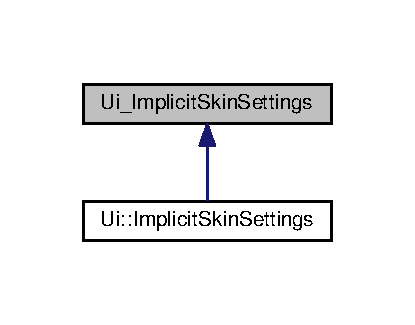
\includegraphics[width=199pt]{d7/dd1/classUi__ImplicitSkinSettings__inherit__graph}
\end{center}
\end{figure}
\subsection*{Public Member Functions}
\begin{DoxyCompactItemize}
\item 
void {\bfseries setup\+Ui} (Q\+Group\+Box $\ast$\hyperlink{classImplicitSkinSettings}{Implicit\+Skin\+Settings})\hypertarget{classUi__ImplicitSkinSettings_abd744cc1ab6638b4b585ab8f6022e214}{}\label{classUi__ImplicitSkinSettings_abd744cc1ab6638b4b585ab8f6022e214}

\item 
void {\bfseries retranslate\+Ui} (Q\+Group\+Box $\ast$\hyperlink{classImplicitSkinSettings}{Implicit\+Skin\+Settings})\hypertarget{classUi__ImplicitSkinSettings_a8d5805215a1a2d44443b20b796af7e6b}{}\label{classUi__ImplicitSkinSettings_a8d5805215a1a2d44443b20b796af7e6b}

\end{DoxyCompactItemize}
\subsection*{Public Attributes}
\begin{DoxyCompactItemize}
\item 
Q\+Grid\+Layout $\ast$ {\bfseries grid\+Layout}\hypertarget{classUi__ImplicitSkinSettings_a4a83141ef631c14d637df7bd3ca572a0}{}\label{classUi__ImplicitSkinSettings_a4a83141ef631c14d637df7bd3ca572a0}

\item 
Q\+Double\+Spin\+Box $\ast$ {\bfseries contact\+Angle}\hypertarget{classUi__ImplicitSkinSettings_ab6b5c7b24e4661c16170de3a1b6cf1ba}{}\label{classUi__ImplicitSkinSettings_ab6b5c7b24e4661c16170de3a1b6cf1ba}

\item 
Q\+Double\+Spin\+Box $\ast$ {\bfseries sigma}\hypertarget{classUi__ImplicitSkinSettings_a4eef0e6dab78595e22eb41d5ecc90ea1}{}\label{classUi__ImplicitSkinSettings_a4eef0e6dab78595e22eb41d5ecc90ea1}

\item 
Q\+Frame $\ast$ {\bfseries line}\hypertarget{classUi__ImplicitSkinSettings_a00b7536407dce65971088f64eaf94cc1}{}\label{classUi__ImplicitSkinSettings_a00b7536407dce65971088f64eaf94cc1}

\item 
Q\+Spacer\+Item $\ast$ {\bfseries vertical\+Spacer}\hypertarget{classUi__ImplicitSkinSettings_ae7e05aead171f155747e733a907a9a32}{}\label{classUi__ImplicitSkinSettings_ae7e05aead171f155747e733a907a9a32}

\item 
Q\+Label $\ast$ {\bfseries label\+\_\+4}\hypertarget{classUi__ImplicitSkinSettings_a6d1040fe8cc0a983139185457c537ffa}{}\label{classUi__ImplicitSkinSettings_a6d1040fe8cc0a983139185457c537ffa}

\item 
Q\+Group\+Box $\ast$ {\bfseries group\+Box}\hypertarget{classUi__ImplicitSkinSettings_a182a4a1a7c3fba2645565dc181089969}{}\label{classUi__ImplicitSkinSettings_a182a4a1a7c3fba2645565dc181089969}

\item 
Q\+Grid\+Layout $\ast$ {\bfseries grid\+Layout\+\_\+2}\hypertarget{classUi__ImplicitSkinSettings_acea165aa16bce4b629718c70ef98d64d}{}\label{classUi__ImplicitSkinSettings_acea165aa16bce4b629718c70ef98d64d}

\item 
Q\+Radio\+Button $\ast$ {\bfseries implicit\+Skin}\hypertarget{classUi__ImplicitSkinSettings_a4e01e5d5bd8a057a86a785826c9c2a0b}{}\label{classUi__ImplicitSkinSettings_a4e01e5d5bd8a057a86a785826c9c2a0b}

\item 
Q\+Radio\+Button $\ast$ {\bfseries lbw\+Skin}\hypertarget{classUi__ImplicitSkinSettings_a74cc443dc7fef52cd88ae427bb4383cf}{}\label{classUi__ImplicitSkinSettings_a74cc443dc7fef52cd88ae427bb4383cf}

\item 
Q\+Label $\ast$ {\bfseries label\+\_\+2}\hypertarget{classUi__ImplicitSkinSettings_a8d97cbadd419cc616547bdefe6ff5924}{}\label{classUi__ImplicitSkinSettings_a8d97cbadd419cc616547bdefe6ff5924}

\item 
Q\+Check\+Box $\ast$ {\bfseries render\+Mesh}\hypertarget{classUi__ImplicitSkinSettings_a24eac49bb9d64e8aaf8675c30fb2dbcb}{}\label{classUi__ImplicitSkinSettings_a24eac49bb9d64e8aaf8675c30fb2dbcb}

\item 
Q\+Label $\ast$ {\bfseries label}\hypertarget{classUi__ImplicitSkinSettings_a72f0077005ce9a1106a87fa1adf12ed7}{}\label{classUi__ImplicitSkinSettings_a72f0077005ce9a1106a87fa1adf12ed7}

\item 
Q\+Push\+Button $\ast$ {\bfseries load\+Animation}\hypertarget{classUi__ImplicitSkinSettings_a8ea8d81bcb21da7fa04e5be6cb17dc60}{}\label{classUi__ImplicitSkinSettings_a8ea8d81bcb21da7fa04e5be6cb17dc60}

\item 
Q\+Spin\+Box $\ast$ {\bfseries iterations}\hypertarget{classUi__ImplicitSkinSettings_ae4148ecc0d799068b4121690b7d5649e}{}\label{classUi__ImplicitSkinSettings_ae4148ecc0d799068b4121690b7d5649e}

\item 
Q\+Line\+Edit $\ast$ {\bfseries animation\+File\+Text}\hypertarget{classUi__ImplicitSkinSettings_ad3f93f890c9406196ff5c8b11582c89f}{}\label{classUi__ImplicitSkinSettings_ad3f93f890c9406196ff5c8b11582c89f}

\item 
Q\+Push\+Button $\ast$ {\bfseries browse\+Animation\+Files}\hypertarget{classUi__ImplicitSkinSettings_a0cb1e6959034f2e675837449b9a1f4dd}{}\label{classUi__ImplicitSkinSettings_a0cb1e6959034f2e675837449b9a1f4dd}

\item 
Q\+Label $\ast$ {\bfseries label\+\_\+3}\hypertarget{classUi__ImplicitSkinSettings_a66598e84fb8b548f6489a73ae231d02e}{}\label{classUi__ImplicitSkinSettings_a66598e84fb8b548f6489a73ae231d02e}

\item 
Q\+Check\+Box $\ast$ {\bfseries wireframe}\hypertarget{classUi__ImplicitSkinSettings_a9537a94d2d8f2c3b8b5de219874a78fd}{}\label{classUi__ImplicitSkinSettings_a9537a94d2d8f2c3b8b5de219874a78fd}

\item 
Q\+Check\+Box $\ast$ {\bfseries iso\+Surface}\hypertarget{classUi__ImplicitSkinSettings_afe4703f23a8869163746da0126c6921c}{}\label{classUi__ImplicitSkinSettings_afe4703f23a8869163746da0126c6921c}

\item 
Q\+Frame $\ast$ {\bfseries line\+\_\+3}\hypertarget{classUi__ImplicitSkinSettings_a01b3ec23016f4f7ea33c70b8e5bcdb43}{}\label{classUi__ImplicitSkinSettings_a01b3ec23016f4f7ea33c70b8e5bcdb43}

\item 
Q\+Frame $\ast$ {\bfseries line\+\_\+2}\hypertarget{classUi__ImplicitSkinSettings_ad720995c211996d0f7f649fd6303a10f}{}\label{classUi__ImplicitSkinSettings_ad720995c211996d0f7f649fd6303a10f}

\end{DoxyCompactItemize}


The documentation for this class was generated from the following file\+:\begin{DoxyCompactItemize}
\item 
ui/ui\+\_\+implicitskinsettings.\+h\end{DoxyCompactItemize}

\hypertarget{classUi__MainWindow}{}\section{Ui\+\_\+\+Main\+Window Class Reference}
\label{classUi__MainWindow}\index{Ui\+\_\+\+Main\+Window@{Ui\+\_\+\+Main\+Window}}


Inheritance diagram for Ui\+\_\+\+Main\+Window\+:\nopagebreak
\begin{figure}[H]
\begin{center}
\leavevmode
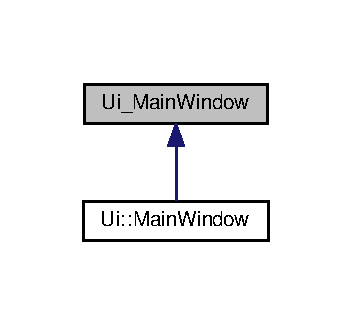
\includegraphics[width=169pt]{d9/dd5/classUi__MainWindow__inherit__graph}
\end{center}
\end{figure}


Collaboration diagram for Ui\+\_\+\+Main\+Window\+:\nopagebreak
\begin{figure}[H]
\begin{center}
\leavevmode
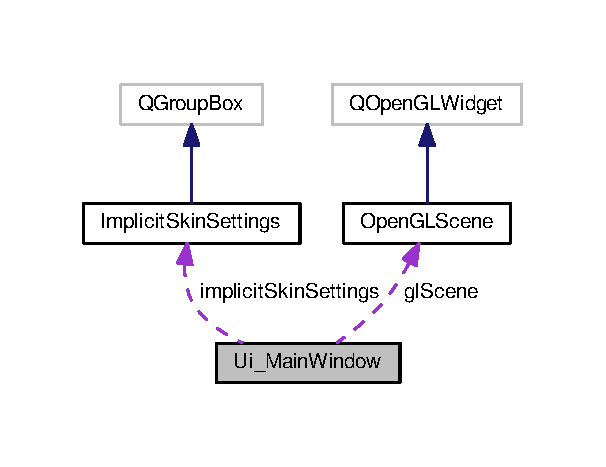
\includegraphics[width=291pt]{d8/d11/classUi__MainWindow__coll__graph}
\end{center}
\end{figure}
\subsection*{Public Member Functions}
\begin{DoxyCompactItemize}
\item 
void {\bfseries setup\+Ui} (Q\+Main\+Window $\ast$\hyperlink{classMainWindow}{Main\+Window})\hypertarget{classUi__MainWindow_acf4a0872c4c77d8f43a2ec66ed849b58}{}\label{classUi__MainWindow_acf4a0872c4c77d8f43a2ec66ed849b58}

\item 
void {\bfseries retranslate\+Ui} (Q\+Main\+Window $\ast$\hyperlink{classMainWindow}{Main\+Window})\hypertarget{classUi__MainWindow_a097dd160c3534a204904cb374412c618}{}\label{classUi__MainWindow_a097dd160c3534a204904cb374412c618}

\end{DoxyCompactItemize}
\subsection*{Public Attributes}
\begin{DoxyCompactItemize}
\item 
Q\+Widget $\ast$ {\bfseries central\+Widget}\hypertarget{classUi__MainWindow_a30075506c2116c3ed4ff25e07ae75f81}{}\label{classUi__MainWindow_a30075506c2116c3ed4ff25e07ae75f81}

\item 
Q\+Grid\+Layout $\ast$ {\bfseries grid\+Layout}\hypertarget{classUi__MainWindow_a525ed3c5fe0784ac502ee222fba4e205}{}\label{classUi__MainWindow_a525ed3c5fe0784ac502ee222fba4e205}

\item 
\hyperlink{classImplicitSkinSettings}{Implicit\+Skin\+Settings} $\ast$ {\bfseries implicit\+Skin\+Settings}\hypertarget{classUi__MainWindow_ad0e50dae1ab8b5118ddecf682a226e18}{}\label{classUi__MainWindow_ad0e50dae1ab8b5118ddecf682a226e18}

\item 
\hyperlink{classOpenGLScene}{Open\+G\+L\+Scene} $\ast$ {\bfseries gl\+Scene}\hypertarget{classUi__MainWindow_a57f629a009e0e3c53e790a4ce9f5a2d3}{}\label{classUi__MainWindow_a57f629a009e0e3c53e790a4ce9f5a2d3}

\item 
Q\+Menu\+Bar $\ast$ {\bfseries menu\+Bar}\hypertarget{classUi__MainWindow_a2be1c24ec9adfca18e1dcc951931457f}{}\label{classUi__MainWindow_a2be1c24ec9adfca18e1dcc951931457f}

\item 
Q\+Tool\+Bar $\ast$ {\bfseries main\+Tool\+Bar}\hypertarget{classUi__MainWindow_a5172877001c8c7b4e0f6de50421867d1}{}\label{classUi__MainWindow_a5172877001c8c7b4e0f6de50421867d1}

\item 
Q\+Status\+Bar $\ast$ {\bfseries status\+Bar}\hypertarget{classUi__MainWindow_a50fa481337604bcc8bf68de18ab16ecd}{}\label{classUi__MainWindow_a50fa481337604bcc8bf68de18ab16ecd}

\end{DoxyCompactItemize}


The documentation for this class was generated from the following file\+:\begin{DoxyCompactItemize}
\item 
ui/ui\+\_\+mainwindow.\+h\end{DoxyCompactItemize}

\hypertarget{structVertexBoneData}{}\section{Vertex\+Bone\+Data Struct Reference}
\label{structVertexBoneData}\index{Vertex\+Bone\+Data@{Vertex\+Bone\+Data}}


Structure to hold bone I\+Ds and bone weights that influence a vertex. Used for Linear Blend Weight(\+L\+B\+W) skinning.  




{\ttfamily \#include $<$mesh.\+h$>$}

\subsection*{Public Attributes}
\begin{DoxyCompactItemize}
\item 
unsigned int \hyperlink{structVertexBoneData_a6629bd01077f6adfbd2e632d71c62acb}{bone\+ID} \mbox{[}Max\+Num\+Blend\+Weights\+Per\+Vertex\mbox{]}\hypertarget{structVertexBoneData_a6629bd01077f6adfbd2e632d71c62acb}{}\label{structVertexBoneData_a6629bd01077f6adfbd2e632d71c62acb}

\begin{DoxyCompactList}\small\item\em m\+\_\+bone\+ID, array of bone ID\textquotesingle{}s that influence this vertex. \end{DoxyCompactList}\item 
float \hyperlink{structVertexBoneData_a2c0bb02c5372c9be2fed58625375ad87}{bone\+Weight} \mbox{[}Max\+Num\+Blend\+Weights\+Per\+Vertex\mbox{]}\hypertarget{structVertexBoneData_a2c0bb02c5372c9be2fed58625375ad87}{}\label{structVertexBoneData_a2c0bb02c5372c9be2fed58625375ad87}

\begin{DoxyCompactList}\small\item\em m\+\_\+bone\+Weight, array of bone weights that control the influence of bones on this vertex. \end{DoxyCompactList}\end{DoxyCompactItemize}


\subsection{Detailed Description}
Structure to hold bone I\+Ds and bone weights that influence a vertex. Used for Linear Blend Weight(\+L\+B\+W) skinning. 

The documentation for this struct was generated from the following file\+:\begin{DoxyCompactItemize}
\item 
include/\+Model/mesh.\+h\end{DoxyCompactItemize}

\hypertarget{structVoxel}{}\section{Voxel Struct Reference}
\label{structVoxel}\index{Voxel@{Voxel}}
\subsection*{Public Attributes}
\begin{DoxyCompactItemize}
\item 
glm\+::vec3 {\bfseries p} \mbox{[}8\mbox{]}\hypertarget{structVoxel_a5084294efff330eafa50a6111422ecba}{}\label{structVoxel_a5084294efff330eafa50a6111422ecba}

\item 
float {\bfseries val} \mbox{[}8\mbox{]}\hypertarget{structVoxel_af542ae384c303a9d4c058052ee16be09}{}\label{structVoxel_af542ae384c303a9d4c058052ee16be09}

\end{DoxyCompactItemize}


The documentation for this struct was generated from the following file\+:\begin{DoxyCompactItemize}
\item 
include/\+Machingcube/Maching\+Cube.\+h\end{DoxyCompactItemize}

\chapter{File Documentation}
\hypertarget{hrbf__phi__funcs_8h}{}\section{include/\+Scalar\+Field/\+Hrbf/hrbf\+\_\+phi\+\_\+funcs.h File Reference}
\label{hrbf__phi__funcs_8h}\index{include/\+Scalar\+Field/\+Hrbf/hrbf\+\_\+phi\+\_\+funcs.\+h@{include/\+Scalar\+Field/\+Hrbf/hrbf\+\_\+phi\+\_\+funcs.\+h}}
This graph shows which files directly or indirectly include this file\+:\nopagebreak
\begin{figure}[H]
\begin{center}
\leavevmode
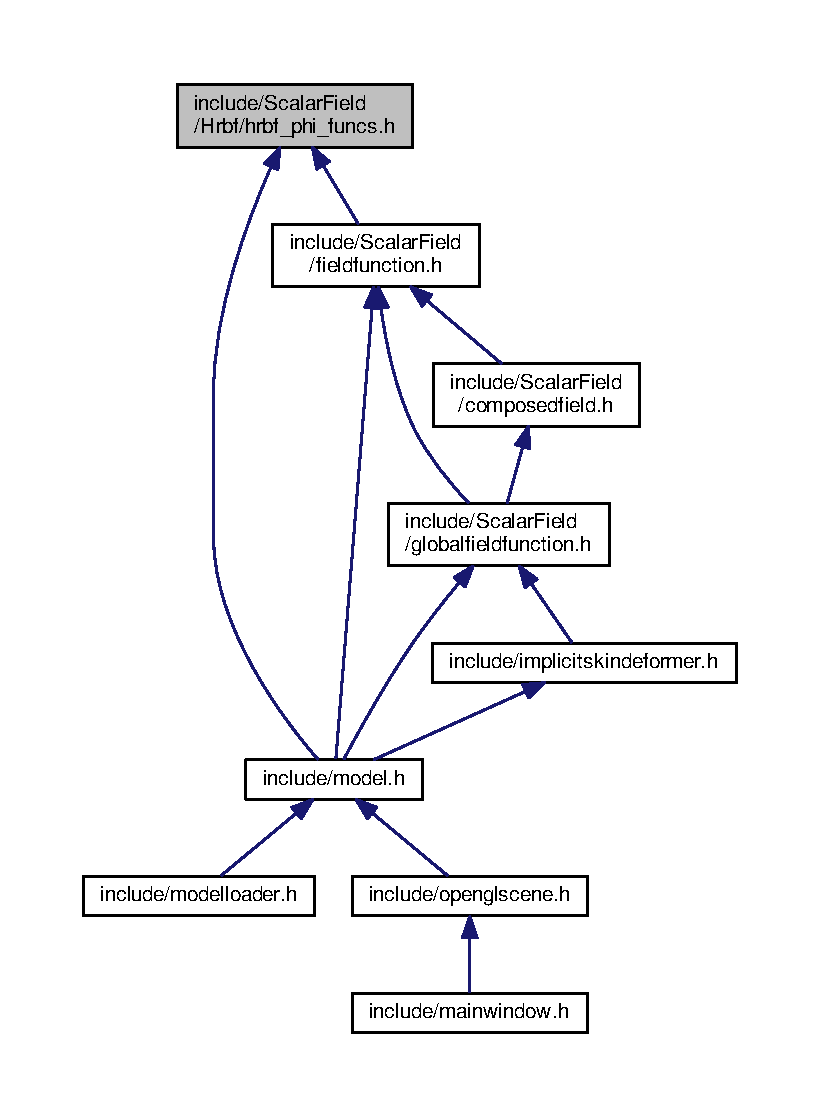
\includegraphics[width=350pt]{d0/d8e/hrbf__phi__funcs_8h__dep__incl}
\end{center}
\end{figure}
\subsection*{Classes}
\begin{DoxyCompactItemize}
\item 
class \hyperlink{structRbf__pow3}{Rbf\+\_\+pow3$<$ Scalar $>$}
\begin{DoxyCompactList}\small\item\em Radial basis functions definitions (function phi) Here you can add more radial basis function definitions. \end{DoxyCompactList}\end{DoxyCompactItemize}


\subsection{Detailed Description}
Original author\+: Gael Guennebaud -\/ \href{mailto:gael.guennebaud@inria.fr}{\tt gael.\+guennebaud@inria.\+fr} -\/ \href{http://www.labri.fr/perso/guenneba/}{\tt http\+://www.\+labri.\+fr/perso/guenneba/} Rodolphe Vaillant -\/ (Fixed the gradient evaluation) -\/ \href{http://www.irit.fr/~Rodolphe.Vaillant}{\tt http\+://www.\+irit.\+fr/$\sim$\+Rodolphe.\+Vaillant} 
\hypertarget{MachingCube_8cpp}{}\section{src/\+Machingcube/\+Maching\+Cube.cpp File Reference}
\label{MachingCube_8cpp}\index{src/\+Machingcube/\+Maching\+Cube.\+cpp@{src/\+Machingcube/\+Maching\+Cube.\+cpp}}


the basic maching cube algorithm  


{\ttfamily \#include \char`\"{}include/\+Machingcube/\+Maching\+Cube.\+h\char`\"{}}\\*
Include dependency graph for Maching\+Cube.\+cpp\+:\nopagebreak
\begin{figure}[H]
\begin{center}
\leavevmode
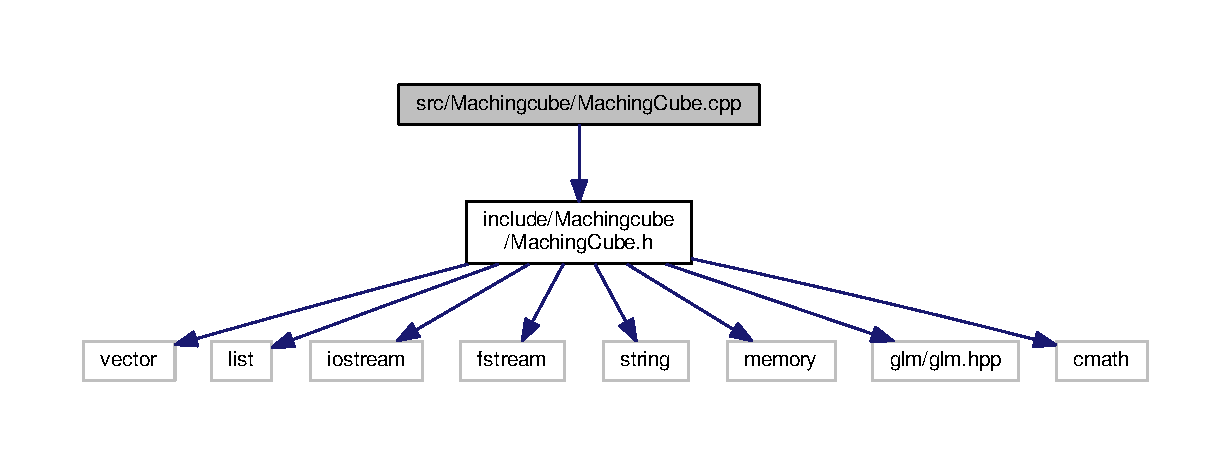
\includegraphics[width=350pt]{d0/dee/MachingCube_8cpp__incl}
\end{center}
\end{figure}


\subsection{Detailed Description}
the basic maching cube algorithm 


%--- End generated contents ---

% Index
\backmatter
\newpage
\phantomsection
\clearemptydoublepage
\addcontentsline{toc}{chapter}{Index}
\printindex

\end{document}
